\documentclass[11pt,a4paper,twoside,openright]{book}
\usepackage{amsmath}
% PAQUETES NECESARIOS
\usepackage[labelsep=period]{caption}
\usepackage{subcaption}
\usepackage{comment}
\usepackage{float}
\usepackage{graphicx}
\usepackage{cancel}
\usepackage[utf8]{inputenc}                 % para poder esribir con acentos
\usepackage[T1]{fontenc}                    % encoding T1 para fonts
\usepackage[english,spanish,es-nodecimaldot]{babel}         % multilenguaje

\usepackage{graphicx}                       % inclusion de figuras 
\usepackage{amsthm, amsmath, amssymb}       % fonts y environments para math
\usepackage{setspace}\onehalfspacing        % espaciado entre lineas
\usepackage[loose,nice]{units}              % units in upright fractions
\usepackage[usarlogouba]{DF-MSc-titlepage}               % titlepage al estilo df.uba.ar
%\usepackage{indentfirst}                    % indentar el inicio de seccion
\usepackage{lipsum}                         % para generar texto generico
%\usepackage{aas_macros}                     % macros para nombre de journals

\usepackage{empheq}                                 %para hacer cajas de texto con color
\usepackage[most]{tcolorbox}

\newtcbox{\mymath}[1][]{%
    nobeforeafter, math upper, tcbox raise base,
    enhanced, colframe=blue!30!black,
    colback=blue!30, boxrule=1pt,
   #1}

\newcommand{\boxedeq}[2]{\begin{empheq}[box={\fboxsep=6pt\fbox}]{equation}\label{#1}#2\end{empheq}}
\newcommand{\coloredeq}[2]{\begin{empheq}[box={\mymath[colback=red!50!black!50!white!50]}]{equation}\label{#1}#2\end{empheq}}


\usepackage{bookmark}                       % para que genere bookmarks en el pdf
\usepackage{fancyhdr}                       % para los headers & footers
\usepackage{emptypage}                      % saca headers and footers de paginas en blanco 
\usepackage{color}
\usepackage{ulem}
\usepackage[margin=1in]{geometry}           % geometria de la pagina 
\usepackage{physics}                        % brakets and such
% CUSTOMIZACIONES PROPIAS
\graphicspath{{./figuras/}}                 % define el directorio de figuras
%\usepackage[Conny]{fncychap}                % para definir estilos de capitulos
%\renewcommand{\vec}[1]{\mathbf{#1}} 	    % vectores como bold
\geometry{bindingoffset=1cm}                % espacio en el borde interno para el encuadernado
\geometry{textwidth=390pt}                  % cuerpo del texto fijo en 390pt
\addto\captionsspanish{\renewcommand{\listtablename}{Índice de tablas}}
\usepackage[svgnames]{xcolor}
\usepackage{hyperref}                       % para vinculos en el pdf
\usepackage{cancel}
\usepackage{bm}
\hypersetup{
    colorlinks=true,
    linkcolor=blue,
    filecolor=magenta,      
    urlcolor=cyan,
    citecolor=Green,
    hyperindex=true,
    pdfauthor={Camila Cristiano},
    pdftitle={Tesis de Licenciatura},
    }

\makeatletter
\def\thickhrulefill{\leavevmode \leaders \hrule height 1ex \hfill \kern \z@}
\def\@makechapterhead#1{%
  %\vspace*{50\p@}%
  \vspace*{10\p@}%
  {\parindent \z@ \centering \reset@font
        \thickhrulefill\quad
        \scshape \@chapapp{} \thechapter
        \quad \thickhrulefill
        \par\nobreak
        \vspace*{10\p@}%
        \interlinepenalty\@M
        \hrule
        \vspace*{10\p@}%
        \Huge \bfseries #1\par\nobreak
        \par
        \vspace*{10\p@}%
        \hrule
    \vskip 40\p@
    %\vskip 100\p@
  }}
\def\@makeschapterhead#1{%
  %\vspace*{50\p@}%
  \vspace*{10\p@}%
  {\parindent \z@ \centering \reset@font
        \thickhrulefill
        \par\nobreak
        \vspace*{10\p@}%
        \interlinepenalty\@M
        \hrule
        \vspace*{10\p@}%
        \Huge \bfseries #1\par\nobreak
        \par
        \vspace*{10\p@}%
        \hrule
    \vskip 40\p@
    %\vskip 100\p@
  }}
\DeclareMathOperator*{\mcm}{mcm}

\titulo{Resumen de papers y resultados de la investigación de doctorado}
\subtitulo{}
\autor{Ali Martin Zynda Aiub}
\numerodelibreta{342/20}
\lugardetrabajo{Departamento de Física, FCEN, UBA}
\director{Dr. Fernando Lombardo}
\codirector{Dra. Paula Villar}
\fechadeinicio{Marzo de 2025}
\fechadefinalizacion{--}
\fechadeexamen{--}



\begin{document}

% Organizacion del manuscrito
%
% Frontmatter
    %\frontmatter
%   Titlepage
    \maketitle
%   Dedication
   \newenvironment{dedicacion}%
{\thispagestyle{empty} \cleardoublepage\null \thispagestyle{empty} \vfill\begin{center}% 
\textbf{} \end{center}}%
{\thispagestyle{empty} \vfill\null }

%\pagestyle{empty}
%\null\vspace{\stretch{1}} 
\begin{dedicacion}
\textit{}



\end{dedicacion}
%{\it
%
%
% 
%}
%\end{flushright}
\vspace{\stretch{2}}\null
%   Resumen (en espanol e ingles)
    \frontmatter
    \spanishlcroman
    \cleardoublepage
\pagenumbering{roman}
\setcounter{page}{1}
%\setcounter{tocdepth}{2}
\tableofcontents

    \listoffigures
    \newenvironment{abstract}%
{\thispagestyle{empty} \cleardoublepage\null \thispagestyle{empty} \vfill\begin{center}
\bfseries \abstractname \end{center} }%
{\thispagestyle{empty} \vfill\null }


\selectlanguage{spanish}
\begin{abstract}


\end{abstract}

%\selectlanguage{english}
%\begin{abstract}



%\end{abstract}
\selectlanguage{spanish}




    \newenvironment{agradecimientos}%
{\thispagestyle{empty} \cleardoublepage\null \thispagestyle{empty} \vfill\begin{center}% 
\textbf{Agradecimientos} \end{center}}%
{\thispagestyle{empty} \vfill\null }

%\pagestyle{empty}
%\null\vspace{\stretch{1}} 
\begin{agradecimientos}
Primero quiero agradecer a Fer, porque siempre estuvo dispuesto a ayudarme y siempre se adapto a mis tiempos y mi ritmo. Gracias a el la tesis se me hizo muy llevadera y sinceramente disfrute el proceso. Tambien quiero agradecer a Pau por sus aportes, y en general a ambos por recibirme en su grupo y darme un proyecto interesante en el cual trabajar. Sin ellos no hubiese sido posible.

A mi familia, Marcelo, Gisela, Mel y Lena.
A Guada.
A mis amigos de la vida Nico, Gunthi, Tincho y Emi.
Y a mis compañeros de la carrera, que hicieron de estos años de estudio una experiencia unica.
Gracias a todos, que contribuyeron en su manera a que esta tesis se haya escrito.



\end{agradecimientos}
%{\it
%
%
% 
%}
%\end{flushright}
\vspace{\stretch{2}}\null

    
%   Tabla de simbolos y notacion (si corresponde)
    
%    \listoftables
% Mainmatter
    \mainmatter
    \pagestyle{fancy}
%   Capitulos de la tesis
    %\pagestyle{fancy}
    % %CAMBIAR ESTO PARA PERSONALIZARLO A MI GUSTO
\pagestyle{fancy}
\fancyhf{}
\fancyhead[LE]{\nouppercase{\rightmark\hfill}}
\fancyhead[RO]{\nouppercase{\leftmark\hfill}}
\fancyfoot[LE,RO]{\hfill\thepage\hfill}


    \chapter{Fases Geometricas: Teoria general}
\label{ch1_fg}


%CAMBIAR ESTO PARA PERSONALIZARLO A MI GUSTO
\pagestyle{fancy}
\fancyhf{}
\fancyhead[LE]{\nouppercase{\rightmark\hfill}}
\fancyhead[RO]{\nouppercase{\leftmark\hfill}}
\fancyfoot[LE,RO]{\hfill\thepage\hfill}

\section{Ecuaciones de FG}

\begin{equation}\label{ec:fg_u_cinematica}
    \phi_u[C]=\arg \bra{\psi(t_i)}\ket{\psi(t)}-\Im \int_{t_i}^{t} dt' \bra{\psi(t_i)}\ket{\dot \psi(t')}
\end{equation}

\begin{equation}
    \phi_g[C]=\arg \sum_{n} \bra{\psi_n(t_i)}\ket{\psi_n(t)} e^{-\Im \int_{t_i}^{t} dt' \bra{\psi_n(t_i)}\ket{\dot \psi_n(t')}}
\end{equation}


    \chapter{Entrelazamiento}
\label{ch2_entrelazamiento}


%CAMBIAR ESTO PARA PERSONALIZARLO A MI GUSTO
\pagestyle{fancy}
\fancyhf{}
\fancyhead[LE]{\nouppercase{\rightmark\hfill}}
\fancyhead[RO]{\nouppercase{\leftmark\hfill}}
\fancyfoot[LE,RO]{\hfill\thepage\hfill}

Entrelazamiento en mecánica cuántica. El entrelazamiento, también conocido como acción espeluznante a la distancia, es un recurso importante en la mecánica cuántica. Este fenómeno no tiene un correlato clásico, ya que lleva a fenómenos que son inexplicables mediante la teórica no cuántica de la física, pero tiene cierta analogía con las correlaciones que se encuentran en la física clásica. El ejemplo mas común de esta analogía es el caso de una masa extensa clásica que está en reposo, y espontáneamente explota mediante procesos internos en dos partes. Imaginemos que esta explosión genera cierto momento angular sobre cada una de las partes. Por conservación del momento angular, que inicialmente es cero, también así lo debe ser luego de la explosión, por lo tanto, si yo me encuentro con uno de estos pedazos de la masa extensa, y le mido su momento angular, se con certeza que el momento angular de la otra masa debe ser exactamente el mismo, pero con signo opuesto para que la suma de momentos angulares sea nula. Lo mismo sucederá con el impulso. Estas cantidades físicas están perfectamente anticorrelacionadas entre si. El entrelazamiento es un fenómeno similar, pero que ciertamente no es el mismo. El entrelazamiento es un fenómeno que es no local. Esto desconcertó a mucha gente, y lo sigue haciendo, pero los experimentos no mienten, y esta es una realidad que tenemos que aceptar. Para dar con esta conclusión y corroborar experimentalmente que el entrelazamiento es un fenómeno no local, hay que mirar el espectacular trabajo de John Bell, físico irlandés de natalidad, al que se le ocurrió un experimento el cual podría ser medido, cuyo resultado daría resultados diferentes dependiendo de si uno acepta o no acepta la no localidad del entrelazamiento. Este experimento fue realizado y se corroboro que efectivamente, la realidad debe ser cuántica y el entrelazamiento es un fenómeno no local. Estas son conocidas como las desigualdades de Bell. 

La verdad que no se para que escribí todo esto pero bueno, lo dejo por acá. Ahora vamos a mirar medidas de entrelazamiento. En particular, estas son sacadas del review de Horodceki$^n$ \cite{quantumentanglementhorodecki}. En la seccion XV.B discuten diferentes medidas de entrelazamiento bipartito, algunas de las cuales se pueden generalizar a estados multipartitos. Cambien, interesantemente, dan una receta para convertir medidas de entrelazamiento para estados puros, generalizandolas para estados mixtos mediante una suma convexa. Sin mas, comencemos.
\section{Medidas de entrelazamiento basadas en distancia}
Esta clase de medidas de entrelazamiento están basadas en la intuición de que un estado separable no esta entrelazado, y si nosotros tenemos una medida de distancia en el espacio de estados, entonces un estado que es muy parecido y por lo tanto esta muy cerca de un estado separable, será poco entrelazado, aumentando esto mientras mas se aleje el estado de algun estado separable. Formalmente podemos decir, dada una medida de distancia $\mathcal{D}$ entre estados en un espacio de estados $\mathcal{S}$, entonces
\begin{equation}
    E_{\mathcal{D},\mathcal{S}}(\rho)=\inf_{\sigma\in\mathcal{S}}\mathcal{D}(\rho,\sigma)
\end{equation}
donde particularmente tenemos que decir quienes son $\sigma\in\mathcal{S}$. El conjunto $\mathcal{S}$ es el conjunto que es cerrado ante operaciones LOCC. Originalmente se consideraba $\mathcal{S}$ como el estado de estados separables. Pero esto no es necesario, o no es algo cierto si se quiere. Esta distnicion surge de que para sistemas de muchas particulas, hay diferentes clases de entrelazamiento, las cuales surgen de clasificar estados segun si podemos transformar un estado en otro mediante LOCC. Es decir, si usando solo LOCC podemos ir de un estado a otro, entonces estos pertenecen a una misma clase. Esta clasificacion hace que haya diferentes tipos de entrelazamiento al aumentar la cantidad de subsistemas, por ejemplo, para un sistema tripartito $\mathcal{H}=\mathcal{H}_1\otimes\mathcal{H}_2\otimes\mathcal{H}_3$. Acá hay algunas tecnicidades sobre la definición de la distancia $\mathcal{D}$, pero no nos vamos a meter en eso. Solo hay que saber que esta tiene que ser no-negativa y que esto implica que la medida de entrelazamiento tiene que ser monotona. La monotonicidad de la medida nos asegura que el entrelazamiento no crece ante LOCC, lo cual es una propiedad necesaria para una medida fiel de entrelazamiento, ya que si operamos con LOCC sobre un estado, siempre deberiamos quedar en la misma clase de entrelazamiento y no deberia aumentar. En \cite{verdalplenio1998} se encontraron dos medidas que satisfacen estas condiciones y ademas son convexas, estas son la métrica de Bures $B^2=2-2\sqrt{F(\rho,\sigma)}$ donde $F(\rho,\sigma)=[\text{Tr}(\sqrt{\rho}\sigma\sqrt{\rho})^{1/2}]^2$ es la fidelidad, y la segunda medida es la entropía relativa $S(\rho|\sigma)=\text{Tr}\rho(\log\rho-\log\sigma)$. Entonces podemos decir que 
\begin{equation}
     E_{\mathcal{D},\mathcal{S}}(\rho)=\inf_{\sigma\in\text{SEP}}\text{Tr}\rho(\log\rho-\log\sigma)
\end{equation}
es la \textit{entropía relativa de entrelazamiento}, que nos sirve como una medida de entrelazamiento, y es una medida fundamental ya que la entropía relativa es una de las funciones mas importantes en la teoría de la información cuántica. Hay otras versiones que calculan la distancia con respecto a los estados PPT \cite{Rains2000} y a los estados nondistillable \cite{Vedral1998}.

Ahora pasamos a ver como generalizar algunas medidas de estados bipartitos a estados multipartitos para estados puros, y luego tenemos que realizar una suma convexa para generalizar a estados mixtos. 

Existen algunas funciones que son sumas de medidas de entrelazamiento bipartito. Por ejemplo \textbf{global entanglement} \cite{MeyerWallach2001} que es la suma de las concurrencias de cada qubit vs los demás, entre otras medidas que son similares. Estas medidas no son una medida real de entrelazamiento multipartito, ya que no consideran entrelazamiento entre k-partes. La primera medida no obvia es el 3-tangle \cite{Coffman2000} 
\begin{equation}
    \tau(A:B:C)=\tau(A:BC)-\tau(AB)-\tau(AC)
\end{equation}
donde los $\tau$s del lado derecho son los 2-tangle, que son el cuadrado de la concurrence. El problema de esta medida es que puede ser 0 para algunos estados que presentan entrelazamiento entre las 3 partes, como los estados W. Por suerte no son cero para los estados GHZ. Aca vemos que el entrelazamiento tripartito tiene dos clases diferentes de estados entrelazados, que en esta medida, uno se pierde de la mitad de los estados. Hay intentos de generalizar esto. En \cite{Lohmayer2006} se computo un convex roof para el 3-tangle para una mezcla de estados GHZ y W. Luego del tangle, se introdujo un concepto para medir en sistemas tripartitos que salio del contexto de asymptotic rate of transitions \cite{Linden1999a}:
\begin{equation}
    E(\psi)=E_R(\rho_{AB})+S(\rho_C)
\end{equation}
donde $\rho_{AB,C}$ son reducciones de $\psi_{ABC}$.

El problema de estas medidas presentadas, es que siempre nos perdemos de alguna propiedad de entrelazamiento, no hay ninguna medida genuina de entrelazamiento tripartito. Busque un poco en internet y encontré un paper de unos chinos \cite{} \text{https://www.polyu.edu.hk/ama/profile/gfzhang/Research/GLW+\_PRA24.pdf} que encuentran una manera genuina de usar alguna medida de entrelazamiento bipartito para obtener una medida de entrelazamiento tripartito. Esta idea se basa en medir el área de un triangulo que representa los entrelazamientos bipartitos del sistema:
\begin{figure}
    \centering
    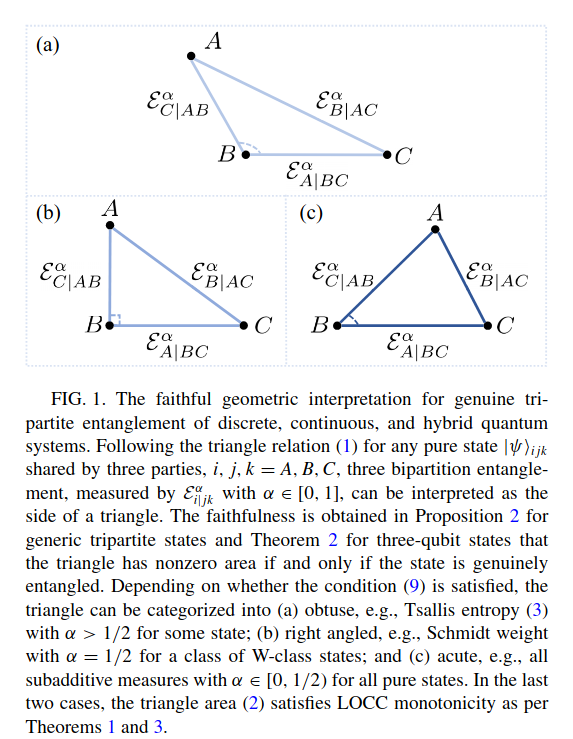
\includegraphics[width=0.5\linewidth]{figuras/ch2/triangulos.png}
    \caption{.}
    \label{fig2:triangulos}
\end{figure}
Lo que dicen es que dada una medida de entrelazamiento bipartito $\mathcal{E}^\alpha_{i|jk}$ definida sobre alguna partición del sistema total $ijk$, lo que se tiene es que
\begin{equation}
    A(\ket\psi_{ijk})=\sqrt{Q(Q-\mathcal{E}^\alpha_{i|jk})(Q-\mathcal{E}^\alpha_{j|ik})(Q-\mathcal{E}^\alpha_{k|ij})}
\end{equation}
con 
\begin{equation}
    Q=(\mathcal{E}^\alpha_{i|jk}+\mathcal{E}^\alpha_{j|ik}+\mathcal{E}^\alpha_{k|ij})/2
\end{equation}
para todo $\alpha\in(0,\frac{1}{2}]$, es una medida genuina de entrelazamiento. Para estados mixtos hacemos una suma usando el formalismo de convex-roof 
\begin{equation}
    A(\rho):= \inf_{\{p_m,\ket\psi_m\}}\sum_m p_m A(\psi_m)
\end{equation}
donde el mínimo es sobre todas las descomposiciones $\rho=\sum_mp_m\ket{\psi_m}\bra{\psi_m}$. Vamos a continuar en ingles para ir practicando escritura. This measure only captures 3-partite entanglement, but forgets about the cases where 2-partite entanglement is present. A trivial example is the case where we have a pure state $\ket{\psi_{EPR}}=\ket{0}\ket{\Phi_{BELL}}$, where $\ket{\Phi_{BELL}}$ is either of the four Bell states. In this trivial example, it is obvious that subsystems 2 and 3 are maximally entangled, but the area of the triangle is 0 because it is separable w.r.t subsystem 1. 

So the first thing to consider when ariving at this expresion is which entanglement measure to use for the bipartitions $\mathcal{E}^\alpha_{i|jk}$. My first two candidates are concurrence and VonNeumann Entropy, but both of them present different kinds of problems. Firstly, concurrence is well known and used for qubit-qubit systems, which is not the case for two of the bipartitions considered here. For concurrence to work, we should generelize it to higher dimensions and it should be able to "distinguish" between 2x2 and 2x3 systems, and have a kind of correspondance between both cases. Secondly, von Neumann entropy is a good measure, but only for pure states. As we have a pure state, perhaps it seems apropiate, but this is not correct because of the fact that the bipartitons of a pure state are not necesarily pure as well. In fact, if we have genuine 3-partite entanglement, it is expected that the reduced density matrices are mixed, and so the von Neuman entropy for the bipartitions is rendered unusable. A quick example shows that the pure state $\ket{GHZ}=(\ket{000}+\ket{111})/\sqrt{2}$ has a reduced density matrix $\rho_{ij}=\text{Tr}_k\ket{\psi}\bra{\psi}=\frac{1}{2}(\ket{00}\bra{00}+\ket{11}\bra{11})$ which is clearly mixed. It is well known that GHZ states are genuinly entangled. Moreover, as we showed, the reduced density matrix is mixed for any bipartition possible, this a hint of the 3-partiness of the entanglement for this particular state. There may be other states that only share entanglement between some parts of the system. A trivial example is en EPR pair of two qubits which we extend to have an aditional part $\ket{EPR}=(\ket{01}+\ket{10})/\sqrt{2}\otimes\ket{i}$. This state only has entanglement between the first two parts of the system. Therefor, not every bipartition of this state is mixed.

The consecuence of this is to look for either a generalized concurrence, for our purpose a qubit-qutrit concurrence will sufice, or to abandon this and use a better measure. As said before, because of the system we are using, and because we want to compute the entanglement for a unitary evolution, it is enough to have a qubit-qutrit entanglement measure, as in the diagonal blocks of the Tavis-Cummings evolution we can at most have a difference in 2 excitations in the cavity field mode. That is, we can think of the cavity as a 3 level system, or in a more inprecise manner, a qutrit. This is only possible if we consider unitary evolution and an initial condition with a well defined number of excitations in the system, so that the evolution reduces to a 3x3 space. It is worth noticing that for this triangle relation to work, the bipartite measure used should work for both $2\otimes2$ and $2\otimes3$ systems, as the bipartitions of the system are not all equal. In the paper that proposed the triangle relation, they examplify the triangle relation with different measures for bipartite entanglement, but most of them are not usefull for mixed states. I think this is wrong, or at least it could be better if we use a measure that can be used for mixed states. 

The triangle area is proved to be a genuine measure for tripartite entanglement insoforth $\mathcal{E}$ is a subadditive measure and $\alpha\in(0,\frac{1}{2}]$, because under this conditions it admits monotonoicity under LOCC.

Another maybe usefull relation for the triangle measure is the fact that they find upper and lower bounds for it:
\begin{equation}
    \min\frac{\sqrt{3}}{4}\{\mathcal{E}^{2\alpha}_{i|jk},\mathcal{E}^{2\alpha}_{j|ik},\mathcal{E}^{2\alpha}_{k|ij}\}\leq A(\ket{\psi}_{ijk})\leq \frac{\mathcal{E}^{2\alpha}_{i|jk}+\mathcal{E}^{2\alpha}_{j|ik}+\mathcal{E}^{2\alpha}_{k|ij}}{4\sqrt{3}}
\end{equation}

Now that, given a good bipartite measure, we have a genuine measure for tripartite entanglement, we must find a good bipartite measure for arbitrary dimension, i.e. a system composed of two qudits with a Hilbert space of dimension $D_1\otimes D_2$. It has to be usefull not only for one selected $D_1$ and $D_2$, but simultaneously for diferent dimensions. Particularly it will suffice that the measure works simultaneously for $2\otimes2$ and $2\otimes D$ dimensions, with $D\geq3$, and it must necesarilly work for mixed states, even if the global evolution remains unitary. 

My quest for a mixed state entanglement measure for a system of arbitrary dimensions starts with I-Concurrence \cite{}, a measure that generalices the concurrence by noting what the concurrence between two qubits represents, and applying this same reasoning to two arbitrary-dimensional systems. The measure comes from the notion that the concurrence is somewhat like the mean value of a inversion operator. As we know, the concurrence for two-qubit system is 

According to \cite{https://scispace.com/pdf/genuine-multipartite-entanglement-detection-and-lower-bound-1j5nw9cffj.pdf} the concurrence for a N-partite pure state $\ket{\psi}\in\mathcal{H}_1\otimes\mathcal{H}_2\otimes...\mathcal{H}_N\otimes$ is 
\begin{equation}
    C_N(\ket{\psi}\bra{\psi})=2^{1-\frac{N}{2}}\sqrt{(2^N-2)-\sum_\alpha \text{Tr}\{\rho_\alpha^2\}}
\end{equation}
If the state is mixed $\rho=\sum_ip_i\ket{\psi_i}\bra{\psi_i}$, then the concurrence is given by the convex roof 
\begin{equation}
    C_N(\rho)=\min_{\{p_i,\ket{\psi_i}\}}\sum_ip_iC_N(\ket{\psi_i}\bra{\psi_i})
\end{equation}
where the minimization is over all possible decompositions of $\rho$ in pure states. 
This makes sense, but why is the concurrence for a qubit-qubit system also well defined for mixed states? 

The concurrence for two bipartite systems can be given in terms of the eigenvalues of a matrix $R=\sqrt{\sqrt{\rho}\tilde\rho\sqrt{\rho}}$ with $\tilde\rho=(\sigma_y\otimes\sigma_y) \rho (\sigma_y\otimes\sigma_y)$. Then the concurrence is defined to be
\begin{equation}
    C(\rho)=\max\{0,\lambda_1-\sum_{i=2}^{\text{rank(R)}}\lambda_i\}
\end{equation}
where $\lambda_i$ are the eigenvalues of the matrix R in descending order $\lambda_1>\lambda_2>...$. 

To understand how to generalize concurrence we shall review how it is defined and it's propoerties following the work of Uhlmann \cite{http://arxiv.org/abs/quant-ph/9909060v4}. Given two vectors $\varphi$, $\psi \in \mathcal{H}\otimes\mathcal{H}^a$, where $\mathcal{H}^a$ is an ancilla, they reduce to 
\begin{align*}
    \rho&=\text{Tr}_a\ket{\varphi}\bra{\varphi} \\
    \omega & = \text{Tr}_a\ket{\psi}\bra{\psi}  
\end{align*}
First we define concurrence between $\rho$ and $\omega$ as
\begin{equation}
    C(\rho,\omega):= \max \{0,\lambda_1-\sum_{j>1}\lambda_j\}
\end{equation}

Then given a conjugation $\Theta$, an
 antiunitary satisfying $\Theta^2 = 1$. Writing $\Theta = \Theta^{-1} = \Theta^\dagger$ shows the hermiticity (self-adjointness) of conjugations. A conjugation $\Theta$ distinguishes in $\mathcal{H}$ a real subspace, $\mathcal{H}_\Theta$,
 consisting of all $\Theta$-invariant vectors, i.e. of all eigenvectors of $\Theta$ with eigenvalue 1. No real subspace in $\mathcal{H}$ is
 properly larger than $\mathcal{H}_\Theta$. Due to Hermiticity, $\Theta \psi = \psi$
 and $\Theta\phi = \phi$ result in
 $\langle\psi,\varphi\rangle=\langle\varphi,\psi\rangle$
 so that the scalar product becomes real if restricted to $\mathcal{H}_\Theta$. In other words, $\mathcal{H}_\Theta$ is not only a real subspace, it is a real Hilbert subspace. On the other hand, $\Theta$ can be gained as complex conjugation in every basis contained
 in $\mathcal{H}_\Theta$. This establishes a one–to–one correspondence between maximal real Hilbert subspaces and conjugations. So, given the conjugation $\Theta$ we define de $\Theta$-Concurrence as 
 \begin{equation}
     C_\Theta(\rho):=C(\rho,\tilde\rho), \; \; \tilde\rho=\Theta\rho\Theta
 \end{equation}
Afterwards they prove some properties and implications.

\textbf{Theorem 1}: Let $\Theta$ be a conjugation, then 
\begin{equation}
    C_\Theta(\rho)=\min\sum|\bra{\phi_k}\Theta\ket{\psi_k}|
\end{equation}
where the \textit{min} is taken over the ensemble $\{\phi_1,\phi_2,...\}$ such that
\begin{equation}
    \rho=\sum\ket{\phi_k}\ket{\psi_k}
\end{equation}
is valid. A direct consequence of the definition of concurrence is homogeneity, given a real numer $\mu$, $C_\Theta(\mu\rho)=\mu C_\Theta(\rho)$ $\forall \mu>0$.

Afterwards it is proven that $C_\Theta$ is \textit{convex}.

Next, we have to see how Optimal Decompositions work. Let $\Omega$ be the state space, if $\rho$ is in this space, a decomposition can be writen as 
\begin{equation}
    \rho=\sum p_k \pi_k, \;\; \pi_k=\frac{\ket{\phi_k}\bra{\phi_k}}{\braket{\phi_k}{\phi_k}}.
\end{equation}
If the decomposition is potimal, the $\Theta$-Concurrence can be writen as
\begin{equation}
    C_\Theta(\rho)=\sum p_kC_\Theta(\pi_k)
\end{equation}
Fixing a density operator $\rho$ and define an antilinear operator $\vartheta$ by
\begin{equation}
    \vartheta \equiv \vartheta_\Theta := \sqrt{\rho}\Theta\sqrt{\rho}.
\end{equation}
Because $\Theta^\dagger=\Theta$, $\vartheta$ is antilinearly Hermitian. The fact that $\Theta=\Theta^\dagger$ means that $\vartheta$ is antilinearly hermitian, then...

Now moving on to the \textbf{generalization of concurrence to more dimensions}, we follow some of the facts and measures used and derived in \cite{arXiv:2208.04745v1  [quant-ph]  2 Aug 2022}. In this work, the authors study the entanglement of certain $2\otimes3$ states, which are called TGX and SGX states. As this states are not of our interest, we will not dive into the details, however they use an entanglement measure that may be usefull for our porupose. Moreover, they give expresions for it and how to perform pure state decomposition. 

\subsubsection{Pure State Decomposition and Convex Roof Extension}\label{subsubsec:convex_roof_ext}

As said, we would like to extend an entanglement measure for pure states to mixed states. This procedure is well known \textit{Convex Roof Extension}, and consists of minimizing over all possible pure decompositions of the mixed state:
\begin{equation}
    E(\rho)=\inf_{\{p_j,\ket{\psi_j}\}}\sum_{j} p_j E(\ket{\psi_j}\bra{\psi_j}).
\end{equation}
To achive this, we have to take the minimum over all posible pure decompositions of the mixed state $\rho$. This could be a daunting task if the Hilbert space is big. The next question is then, how to find all pure decompositions of a given density matrix. A way to, do this is to take $\rho$ to its spectral decomposition. It is one of the posible pure decompositions:
\begin{equation}
    \rho=\sum\lambda_i\ket{\phi_i}\bra{\phi_i}
\end{equation}
where $\{\lambda_i,\ket{\phi_i}\}$ are the eigenvalues and corresponding eigenvectors of $\rho$. Then, we can take a unitary transformation defined by its matriz elements $U_{jk}$ and define a set of modified vectors
\begin{equation}
    \ket{\tilde w_j}=\sum_k U_{jk}\sqrt{\lambda_k}\ket{\phi_k}.
\end{equation}
Given this new vectors we can arrive at another expresion for the density matrix
\begin{equation}
    \rho=\sum_j p_j \ket{w_j}\bra{w_j},
\end{equation}
where $p_j=\braket{\tilde w_j}{\tilde w_j}$ and $\ket{w_j}=1/\sqrt{p_j}\ket{\tilde w_j}$. This means that we have a expresion that depends on the unitary transformation $U$:
\begin{equation}
    E(\rho)=\inf_{\{U\}} \sum p_j E(\ket{w_j}\bra{w_j}),
\end{equation}
where now the minimum is taken over all posible unitary transformations $U$. This means, our task is to minimize this function over all $U\in U(6)$, the unitary group $U(6)\in \mathbb{C}^{6\times6}$. The first thing to attempt is to parametrize this matrix group, but this turns out to be impossible, so the next step is to find a way to sample and take the minimum of this function over all possible $U$. This leads us to Random Matrix Theory (RMT), a usefull tool for this kinds of problems, where we have to evaluate a funtion over the manifold of unitary matrices. This is an interesting topic, but it will suffice to find some numerical way to randomly generate a matrix and some numerical way to span the manifold. For this, we found the python libraries \textit{pymanpot} \cite{JMLR:v17:16-177} and \textit{geomstats}, which in combination give us the numerical tools to explore the whole matrix manifold and optimize this function in a spart way, for example using gradiente descendiente and not only brute force. 

\section{Exploring optimization algorithms for entangled mixed states}

As in section \ref{subsubsec:convex_roof_ext}, we want to find the convex roof extension for the tripartite case. Therefor, we use Pymanopt and Autograd to solve this optimization problem in Python. 

To se which optimization algorithm implemented here works best, we will compute the entanglement of the 4x4 reduced density matrix of the two qubits tracing over the cavity $\rho_{AB}=\text{Tr}_C(\ket{\psi}\bra{\psi})$. As for a mixed two qubit state we can use the Conncurrence as a measure for entanglement, we will compare the Convex roof extension optimizatino for different measures and algorithms to see what combination is closer to the concurrence. With this analysis we will choose the best combination available to study tripartite entanglement. 
First using von Neuman entropy and Conjugate Gradient optimizer, we study if the parameter \textit{min\_step\_size} improves the algorithm. 


For now, the best algorithm seems to be the ParticleSwarm, using parameters max\_iterations=5 and population=25 seems reasonable, as it give good results and is not as computationally costly. Either way, the problem is that comparing the numerics, the convex roof extension is noisy in comparision to concurrence, and moreover it does not present entanglement sudden death. 

As this aproach seems to be numerically unstable and costly, we look for other alternatives. 

The next thing I found is Negativity. It seems to work for any bipartite system, independent of the dimensions, and doing some quick test, it also presents entanglement sudden death. As this seems to work, the next step is to try to make a tripartite entanglement measure using negativity, and doing an analysis of the dependence of the entanglement on the parameters of the problem. 

The main thing to look out for, is how we quantify the entanglement, since we have different kinds of entanglement in the system, that is, between any two parties, for example between A and B but tracing over C, then we have entanglement between A and B+C, and finally we have genuine tripartite entanglement. In total, 7 different kinds of entanglement. 
Another interesting question: Is it possible to find an entanglement invariant? Or some quantity that is invariant if the entanglement of the system remains constant? The goal of this is to see if during the evolution, the entanglement varies. Obviously, as it is easily available with numerics, the entanglement of the subsystems does change, but we do not have a precise defiintion of what entanglement means in this tripartite case. Maybe, if we have a general quantity that we now is entanglement invariant (whatever entanglement means in whatever dimension we are treating), it can tell us if the systems entanglement is actually changing or not.

\subsubsection{Negativity}\label{subsubsec:negativity}
La negatividad sirve para ver cuanto un estado esta de distancia a uno separable, usando la transposicion parcial. Esta caracteristica funciona porque las matrices densidades tienen que ser semidefinidas positivas, y la operacion transposicion parcial nos lleva de estados separables a estados separables, en este caso, siendo la matriz transpuesta parcialmente tambien una matriz (o observable) positivo. En cambio, si aplicamos la transposicion parcial sobre un estado entrelazado, entonces la matriz densidad resultante no es positiva, entonces si hacemos la suma de los autovalores negativos, tenemos una medida de cuanto el estado se aleja de ser separable. Formalmente, la negatividad se define como
\begin{equation}
    \mathcal{N}(\rho)=\sum_{\lambda<0}|\lambda|=\frac{||\rho^{T_A}||_1-1}{2}
\end{equation}
donde $||\cdot||_1$ es la norma 1, que es la suma de los valores absolutos de los autovalores, y $\rho^{T_A}$ es la transposicion parcial de $\rho$ sobre el sistema A. Esta medida es una buena medida de entrelazamiento, ya que es monotona bajo LOCC, y es computacionalmente simple. Cuando consideramos estados multipartitos, la negatividad no nos da una medida genuina de entrelazamiento entre las 3 partes, pero si nos da una idea de cuanto entrelazamiento hay entre dos partes del sistema. En este caso, hay 6 particiones o situaciones posibles. Las primeras tres constan en pensar el entrelazamiento que comparten A-(BC), es decir la negatividad de la matriz total $\rho_{ABC}$ traspuesta parcialmente sobre A, y lo mismo para B-(AC) y C-(AB). Estas tres particiones nos dan una idea de cuanto entrelazamiento hay entre una parte del sistema y las otras dos. Luego, tenemos las otras tres particiones, que son A-B (trazando sobre C), B-C (trazando sobre A) y A-C (trazando sobre B). Estas tres particiones nos dan una idea de cuanto entrelazamiento hay entre dos partes del sistema, considerando que la tercera no coopera en el sentido de LOCC, por lo tanto las otras dos partes pierden una parte del entrelazamiento (o no). 
Hay diferentes criterios de separabilidad y clasificaciones de entrelazamiento, que se pueden resumir con la siguiente tabla:
\begin{table}
    \centering
    \begin{tabular}{|c|c|c|c|c|}
    \hline
         & $E_A$ & $E_B$ & $E_C$ & $\tau_3$ \\
         \hline
         A-B-C & 0 & 0 & 0 & 0 \\
         \hline
         A-BC & 0 & >0 & >0 & 0\\
         \hline
         B-AC & >0 & 0 & >0 & 0\\
         \hline
         C-AB & >0 & >0 & 0 & 0\\
         \hline
         W & >0 & >0 & >0 & 0\\
         \hline
         GHZ & >0 & >0 & >0 & >0\\
    \hline
    \end{tabular}
    \caption{Clasificacion de entrelazamiento en sistemas tripartitos.}
    \label{tab:entrelazamiento_tripartito}
\end{table}
Realizando esto sobre nuestro sistema, obtenemos los siguientes resultados.
Primero veamos para condicion inicial $\frac{1}{\sqrt{2}}(\ket{eg1}+\ket{ge1})$, comenzando por lo mas similar a lo que teniamos antes, el entrelazamiento entre los dos atomos trazando sore la cavidad, esto lo llamamos $N_{01}$. Tambien tenemos la posibilidad de estudiar el entrelazamiento entre un atomo y la cavidad, trazando sobre el otro atomo, que llamamos $N_{02}$ y $N_{12}$. Esperamos que $N_{02}=N_{12}$ por la simetria del estado inicial. Finalmente tenemos la posibilidad de estudiar el entrelazamiento entre un atomo y el resto del sistema, que llamamos $N_0$ y $N_1$, y el entrelazamiento entre la cavidad y los dos atomos, que llamamos $N_2$.

En cada subplot variamos $\Delta$, y vemos que tambien vamos variando $\chi$ y $k-J$ segun vamos moviendonos para la izquierda o hacia abajo respectivamente. En estas simulaciones los valores de $\chi$ y $k-J$ son en cada direccion $a=0,g,2g$ para $a=\chi,k-J$. Tambien como comentario general para esta serie de graficos, notemos que la barra de colores esta normalizada diferente para cada grafico, esto se debe a que en algunos casos, no se alcanzan valores entre 0 y 1, y por lo tanto no se aprecian correctamente las oscilaciones, de esta manera, se contrasta mejor pero hhay que estar atentos a eso.
\begin{figure}
    \centering
    \includegraphics[width=0.8\linewidth]{figuras/ch2/negatividad/3x3 eg1+ $N_{01}$ 012 012.png}
    \caption{Negatividad $N_{01}$ para condicion inicial $\frac{1}{\sqrt{2}}(\ket{eg1}+\ket{ge1})$.}
    \label{fig2:N_01_eg1+}
\end{figure}
Vemos que estos graficos son muy similares a los que teniamos antes con la concurrence, donde encontramos estas regiones "interesantes". La diferencia principal es que la negatividad no va entre 0 y 1 como la concurrence, sino que va entre 0 y $1/2$. Aun asi es similar el comportamiento.  
\begin{figure}
    \centering
    \includegraphics[width=0.8\linewidth]{figuras/ch2/negatividad/3x3 eg1+ $N_{02}$ 012 012.png}
    \caption{Negatividad $N_{02}$ para condicion inicial $\frac{1}{\sqrt{2}}(\ket{eg1}+\ket{ge1})$.}
    \label{fig2:N_02_eg1+}
\end{figure}

\begin{figure}
    \centering
    \includegraphics[width=0.8\linewidth]{figuras/ch2/negatividad/3x3 eg1+ $N_{12}$ 012 012.png}
    \caption{Negatividad $N_{12}$ para condicion inicial $\frac{1}{\sqrt{2}}(\ket{eg1}+\ket{ge1})$.}
    \label{fig2:N_12_eg1+}
\end{figure}
Como es de esperar, los graficos de $N_{02}$ y $N_{12}$ son iguales, por la simetria del estado inicial. En estos casos, la negatividad parece casi contraria a la de $N_{01}$, en donde en uno vemos una zona muy oscura, donde hay muchoi entanglement sudden death, en el otro vemos oscilaciones de gran amplitud y no mucho sudden death. Esto lleva a pensar que el entrelazamiento se va pasando de uno al otro. Para comprobar esto deberiamos hacer un grafico mostrando la suma de los entrelazamientos a ver si se mantiene aproximadamente constante. La otra cosa a destacar es que las oscilaciones en estos dos graficos van entre 0 y 0.3, a diferencia del anterior donde oscilan entre 0 y 0.5. 

Ahora miremos las negatividades entre un subsistema con los otros dos, que son las cantidades $N_0$, $N_1$ y $N_2$. Estas representan, por ejemplo el $N_0$, el entrelazamiento entre el primer atomo y el resto del sistema, es decir el segundo atomo y la cavidad. Nuevamente esperamos que $N_0=N_1$ por la simetria del estado inicial. Esto parece efectivamente ser asi.
\begin{figure}
    \centering
    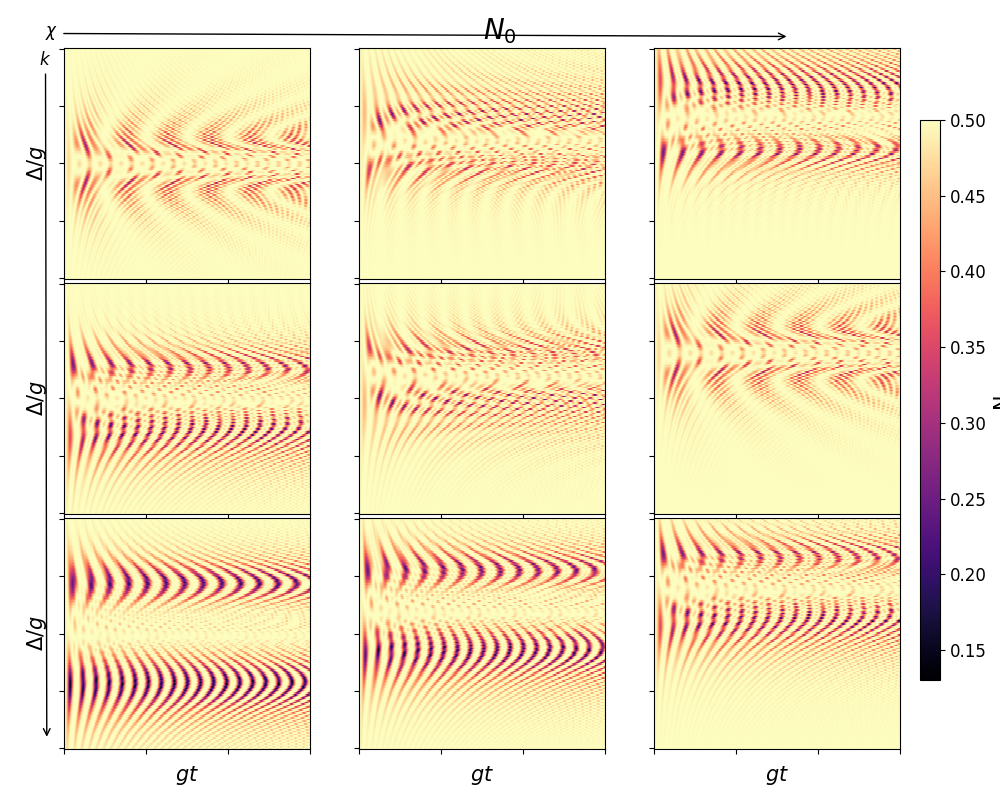
\includegraphics[width=0.8\linewidth]{figuras/ch2/negatividad/3x3 eg1+ $N_0$ 012 012.png}
    \caption{Negatividad $N_{0}$ para condicion inicial $\frac{1}{\sqrt{2}}(\ket{eg1}+\ket{ge1})$.}
    \label{fig2:N_0_eg1+}
\end{figure}

\begin{figure}
    \centering
    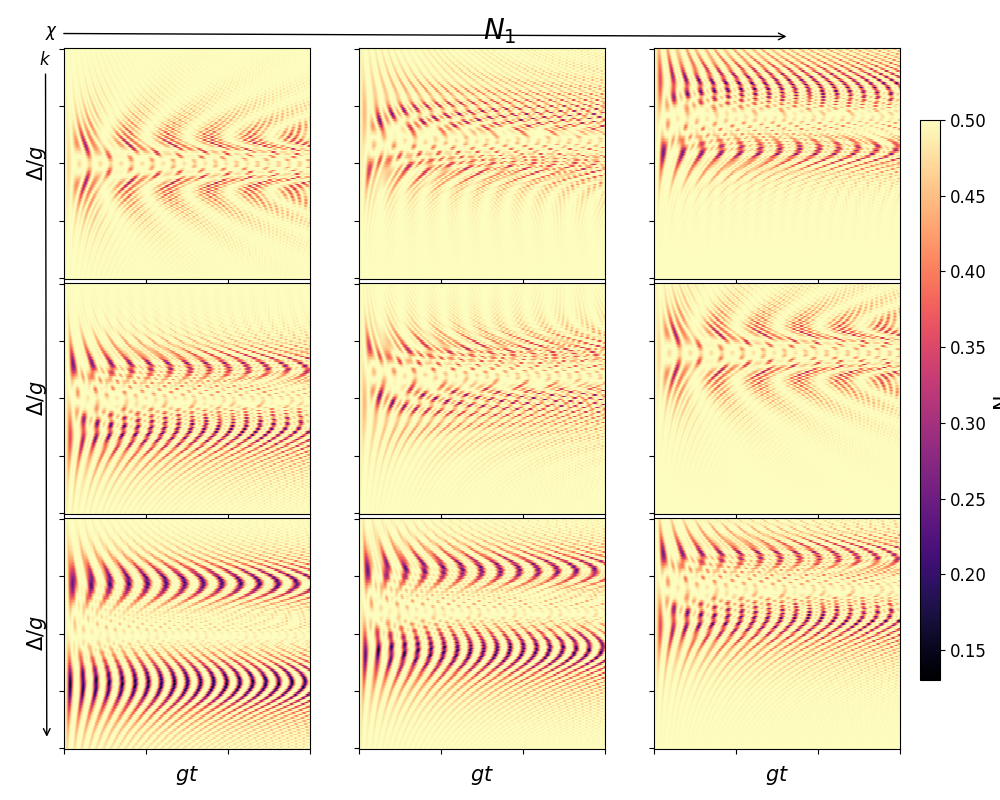
\includegraphics[width=0.8\linewidth]{figuras/ch2/negatividad/3x3 eg1+ $N_1$ 012 012.png}
    \caption{Negatividad $N_{1}$ para condicion inicial $\frac{1}{\sqrt{2}}(\ket{eg1}+\ket{ge1})$.}
    \label{fig2:N_1_eg1+}
\end{figure}
Mirando estos dos graficos, podemos observar como hay entrelazamiento bastante fuerte, y tambien vemos regiones oscilantes. Esto habria que analizarlo un poco mas en detalle pero esta interesante.
\begin{figure}
    \centering
    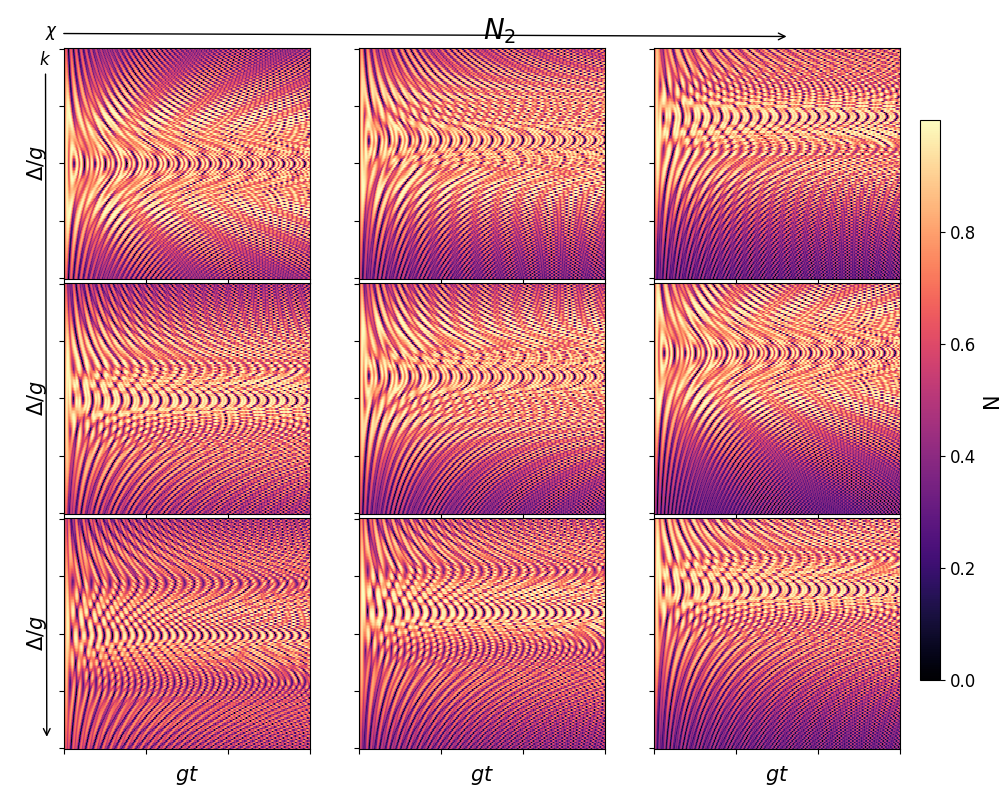
\includegraphics[width=0.8\linewidth]{figuras/ch2/negatividad/3x3 eg1+ $N_2$ 012 012.png}
    \caption{Negatividad $N_{2}$ para condicion inicial $\frac{1}{\sqrt{2}}(\ket{eg1}+\ket{ge1})$.}
    \label{fig2:N_2_eg1+}
\end{figure}
A diferencia del anterior, en este caso parece que mientras maor sea el detunning, menor es el entrelazamiento que comparte la cavidad con el resto del sistema, pero aun asi debemos diferenciar que en este grafico los colores estan normalizados entre practicamente 0 y 1, con lo cual quizas es un poco enganioso y hay que rehacer los graficos con la misma escala de colores para poder comparar un poco mejor.

Lo ultimo que tengo para decir es que, estaria bueno hacer un codiguito para estudiar lo que esta puesto en la tabla \ref{tab:entrelazamiento_tripartito}, donde nos fijamos tiempo a tiempo si las 3 negatividades son mayores a cero. Esto nos va a decir si hay entrelazamiento tripartito, o si solo hay entrelazamiento bipartito que se va moviendo entre las partes. Yo espero que haya algun entrelazamiento tripartito pero estaria bueno tener un grafico concreto que nos muestre con certeza. 

Las conclusiones son que podemos extender un poco mas el analisis del entrelazamiento que habiamos hecho antes. Todavia me queda estudiarlo a fondo, pero estaba mas concentrado en los otros proyectos y en leer otras cosas porque estaba un poco cansado y queria leer cosas nuevas. Pero ahora que hace algunas semanas que no lo toco mucho esto, me dieron ganas de analizar bien en profundidad esto y ver si podemos sacar una conclusion un poco mas fuerte. 

Tambien tenemos para otra condicion inicial. Los graficos van todos juntos en el apendice \ref{a}
\subsubsection{Schmidt Decomposition}
\text{https://arxiv.org/pdf/quant-ph/0610253} paginas 53-60 aprox

Se puede ver si queda invariante durante la evolucion. No deberia porque el entrelazamiento va cambiando, pero quizas es interesante ver como hace. Esta medida no es continua, ya que se basa en la descomposicion de schmidt y busca ver cual es el minimo posible de estados necesarios en la descomposicion. Entonces si es separable deberiamos tener $E_S=log_2(1)=0$, pero apenas sea un poquito entrelazado tenemos $E_S=log_2(2)=1$. Depende del tipo de entrelazamiento podesmo tener diferentes valores de $E_S$, pero son discontinuos.

\subsubsection{Ent: A Multipartite Entanglement Measure, and Parameterization of Entangled States}

Hoy encontre un paper que parece interesante. Lo tengo que leer a ver si me gusta y me convence. Escrito por  Samuel R. Hedemann  arXiv:1611.03882v3  [quant-ph]  18 Apr 2018.



    \chapter{Fase geométrica en JCM generalizado}
\label{ch5:fgdoble}


%CAMBIAR ESTO PARA PERSONALIZARLO A MI GUSTO
\pagestyle{fancy}
\fancyhf{}
\fancyhead[LE]{\nouppercase{\rightmark\hfill}}
\fancyhead[RO]{\nouppercase{\leftmark\hfill}}
\fancyfoot[LE,RO]{\hfill\thepage\hfill}
Este capítulo se divide en dos partes. En la primera se estudia la dependencia de la FG con los parámetros del problema, y se analizan situaciones de robustez, intentando ver si las condiciones halladas en el capítulo anterior predicen correctamente dichas características. En la segunda parte, se examina en detalle la robustez para varias condiciones iniciales diferentes, pero siempre en función del detunning, ya que este es el parámetro más accesible experimentalmente.

\section{Dependencias de la FG}

Se estudia la dependencia de la fase geométrica con los distintos parámetros del problema, siguiendo la definición de la FG en Ec. (\ref{ec:fg_u_cinematica}). Se estudian los efectos en cada caso, y se buscan condiciones de robustez. Nuevamente, se estudian las condiciones iniciales $\frac{1}{\sqrt{2}}(\ket{eg0}+\ket{ge0})$, $\frac{1}{\sqrt{2}}(\ket{eg1}+\ket{ge1})$ y $\ket{gg2}$, con el objetivo de recuperar comportamientos similares al JCM de 1 átomo para el primer caso, y comparar estos con el otro. 

\subsection{Dependencia con el régimen de acoplamiento}

En la figura \ref{fig5:dependencia acoplamiento} se observa la fase geométrica acumulada para diferentes valores del acoplamiento con el entorno $\gamma=0, 0.01g,0.1g,0.5g,g$, donde cada valor se corresponde con una curva mostrada, en orden ascendente en la luminosidad de los colores. Es decir, $\gamma=0$ se corresponde con la curva azul oscuro, y $\gamma=g$ con el color más claro (naranja). El comportamiento para la condición inicial $\frac{1}{\sqrt{2}}(\ket{eg0}+\ket{ge0})$ mostrado en la figura \ref{fig5:dependencia acoplamiento eg0} es idéntico al caso del JCM de 1 átomo, donde aumentar la disipación hace que los escalones se suavicen, y dejen de acumular fase rápidamente por la destrucción de las coherencias. 

\begin{figure}[h]
    \centering
    \begin{subfigure}{0.49\textwidth}
        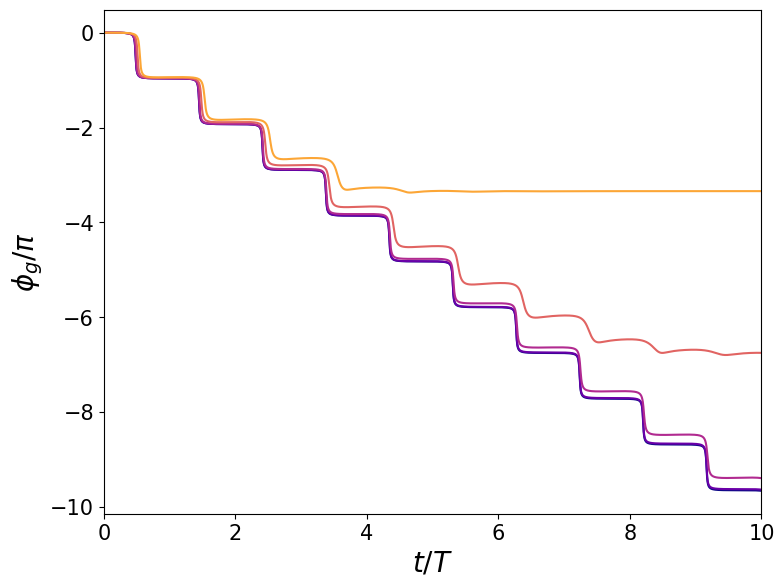
\includegraphics[width=\textwidth]{figuras/ch5/dependencia/eg0+/acoplamiento d=0.1g.png}
        \caption{}
        \label{fig5:dependencia acoplamiento eg0}
    \end{subfigure}
    \hfill
    \begin{subfigure}{0.49\textwidth}
        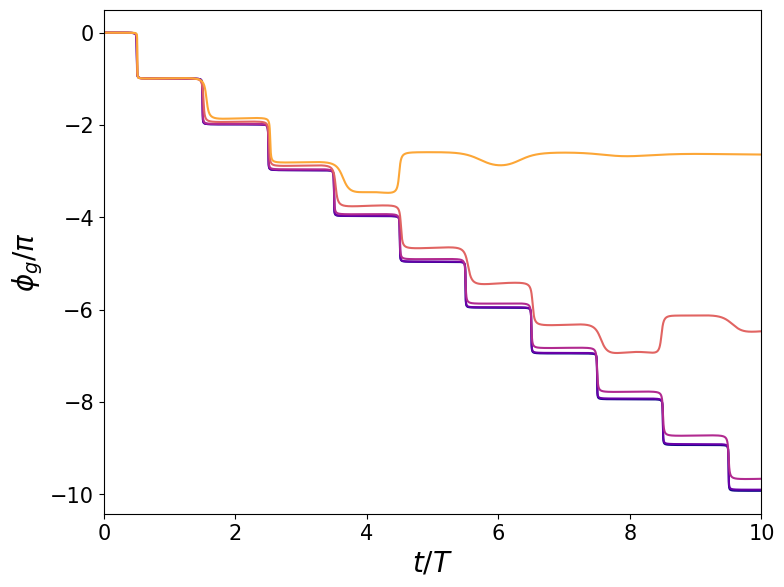
\includegraphics[width=\textwidth]{figuras/ch5/dependencia/eg1+/acoplamiento d=0.1g.png}
        \caption{}
        \label{fig5:dependencia acoplamiento eg1}
    \end{subfigure}
    \caption{Dependencia de la FG acumulada con el acoplamiento con el entorno para condiciones iniciales (a) $\frac{1}{\sqrt{2}}(\ket{eg0}+\ket{ge0})$ y (b) $\frac{1}{\sqrt{2}}(\ket{eg1}+\ket{ge1})$.}
    \label{fig5:dependencia acoplamiento}
\end{figure}
En el caso de la condición inicial correspondiente al subespacio de $N=2$, se observa un nuevo comportamiento: un \textit{rebote}. Al aumentar lo suficiente el acoplamiento con el entorno, la acumulación de fase geométrica hace un salto en la dirección contraria a la que lleva normalmente, y luego oscila cerca a su valor asintótico. Como se vio anteriormente, los saltos que hacen aparecer los escalones, se podían interpretar en el caso de 1 átomo utilizando la esfera de Bloch. Estos saltos ocurren cuando la trayectoria llega al otro lado de la esfera de Bloch. Al llegar al lado opuesto (digamos $\phi=\pi$), justo al superar este punto, el camino más corto para cerrar el ciclo, según la regla de la geodésica, es recorrer la esfera por el otro lado, dando así un salto de $\pi$ en el caso resonante. Esta interpretación en el caso de un espacio de Hilbert más extenso no es tan directa, pero se puede pensar en analogía en una esfera de mayor dimensión, en donde el rebote sería una situación similar a la descrita anteriormente. Más allá de esto, el comportamiento es el esperado, e incluso se ve que ambos casos acumulan una fase geométrica muy similar en términos de su valor absoluto. No parece haber diferencias significativas en la influencia que tiene el entorno sobre estos dos estados.

\subsection{Dependencia con el detunning}
%delta list=(0.00001*g,0.1*g,0.500001*g,1.00001*g,1.500001*g,2.5*g,5*g)

Para estudiar el efecto del detunning sobre la fase geométrica, se dejan fijos los otros parámetros del problema y se varía la diferencia entre las frecuencias de los átomos y la cavidad. Como el régimen de acoplamiento fuerte es el que nos interesa, se elije un acoplamiento con el entorno $\gamma=0.1g$ y $p=0.005g$, y en un principio los demás parámetros en cero $\chi=k-J=0$. En la figura \ref{fig5:dependencia detunning} se muestran la fase acumulada para diferentes valores del detunning $\Delta$ para las dos condiciones iniciales elegidas. En \ref{fig5:dependencia detunning eg0} se observa el mismo comportamiento que en el caso de 1 átomo, el detunning hace que los escalones sean más suaves y el salto menor, haciendo que en conjunto el sistema acumule menos fase geométrica. Si asociamos la fase geométrica al camino que recorre el estado en el espacio de estados, es evidente que a mayor detunning, la fase acumulada será menor, ya que como se mencionó en reiteradas ocasiones, al aumentar el detunning las oscilaciones entre los estados son más pequeñas, y por lo tanto la probabilidad está concentrada en la condición inicial. Consecuentemente, en el espacio de rayos, la curva se mantiene cerca del origen y, por lo tanto, la fase acumulada es menor. En el caso de la condición inicial en el subespacio de $N=2$, si el detunning es bajo, entonces el efecto es similar al anterior y la fase acumulada tiene una forma y un valor similar. Pero aproximadamente en el rango de $1g \leq \Delta \leq 5g$, hay una gran diferencia. La fase acumulada es más errática y presenta saltos y \textit{rebotes}. Al seguir aumentando el detunning, estos parecen disminuir y converger al comportamiento esperado para un detunning grande: que la fase acumulada sea poca.
\begin{figure}[h]
    \centering
    \begin{subfigure}{0.49\textwidth}
        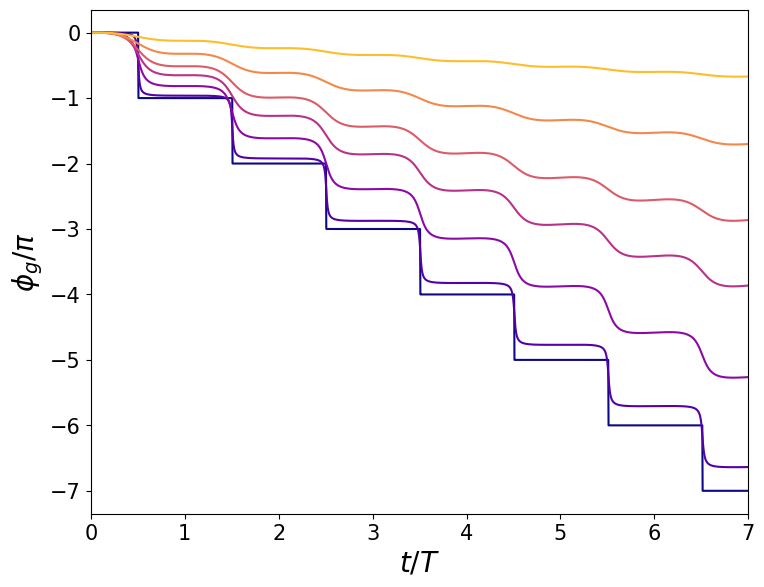
\includegraphics[width=\textwidth]{figuras/ch5/dependencia/eg0+/detunning todo 0.png}
        \caption{}
        \label{fig5:dependencia detunning eg0}
    \end{subfigure}
    \hfill
    \begin{subfigure}{0.49\textwidth}
        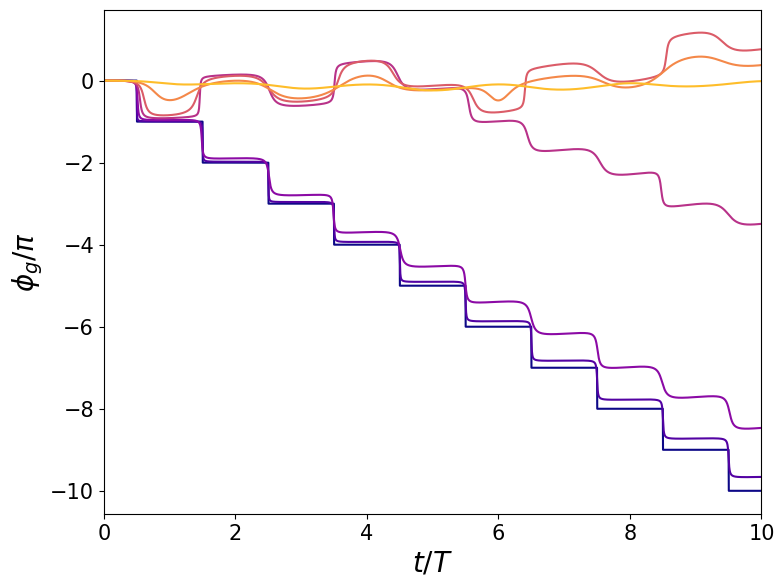
\includegraphics[width=\textwidth]{figuras/ch5/dependencia/eg1+/detunning todo 0.png}
        \caption{}
        \label{fig5:dependencia detunning eg1}
    \end{subfigure}
    \caption{Dependencia de la FG acumulada con el detunning para condiciones iniciales (a) $\frac{1}{\sqrt{2}}(\ket{eg0}+\ket{ge0})$ y (b) $\frac{1}{\sqrt{2}}(\ket{eg1}+\ket{ge1})$.}
    \label{fig5:dependencia detunning}
\end{figure}
Una explicación para el comportamiento en el rango medio de detunning es que las poblaciones comienzan a presentar batidos. Las probabilidades de los estados $\ket{ee0}$ y $\ket{gg2}$ comienzan a aumentar y son comparables a la probabilidad del estado inicial. Esto hace que en el espacio de estados, las curvas sean complicadas y tengan trayectorias largas, haciendo que en algunos casos el salto sea positivo, y en otros, negativo. Para valores de detunning bajos, el sistema principalmente se centra en el estado $\frac{1}{\sqrt{2}}(\ket{eg1}+\ket{ge1})$, y para detunnings altos también. Es en este rango intermedio, que las amplitudes de los 3 estados sin similares y oscilan de manera errática, presentando batidos, y por eso la fase geométrica acumulada no sigue un comportamiento continuo a lo largo de su dependencia con el parámetro. 
No se encontró una manera clara de representar ésto en el espacio de parámetros para poder entender intuitivamente el comportamiento, ya que la esfera de Bloch no es una herramienta que se pueda utilizar en esta situación. 
Para seguir el estudio, se presenta la diferencia entre la fase geométrica unitaria y la disipativa en función del detunning. Para ello se realizan simulaciones para diferentes valores de $\Delta$ y se compara el valor de la fase geométrica luego de un tiempo fijo $t=3T$ para dos casos, el primero presentando pérdidas y el segundo sin pérdidas. Luego se realiza la resta de ambas cantidades y se obtiene el gráfico \ref{fig5:robustez detunning eg0}.

\begin{figure}[h]
    \centering
    \begin{subfigure}{0.49\textwidth}
        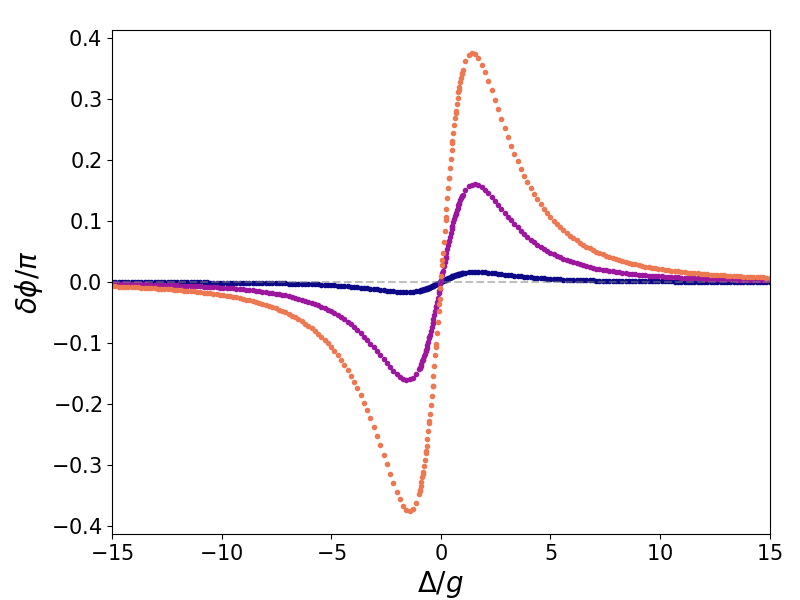
\includegraphics[width=\textwidth]{figuras/ch5/robustez/delta/eg0+ge0 k=0.0g x=0.0g J=0.0g.png}
        \caption{}
        \label{fig5:robustez detunning 1 eg0}
    \end{subfigure}
    \hfill
    \begin{subfigure}{0.49\textwidth}
        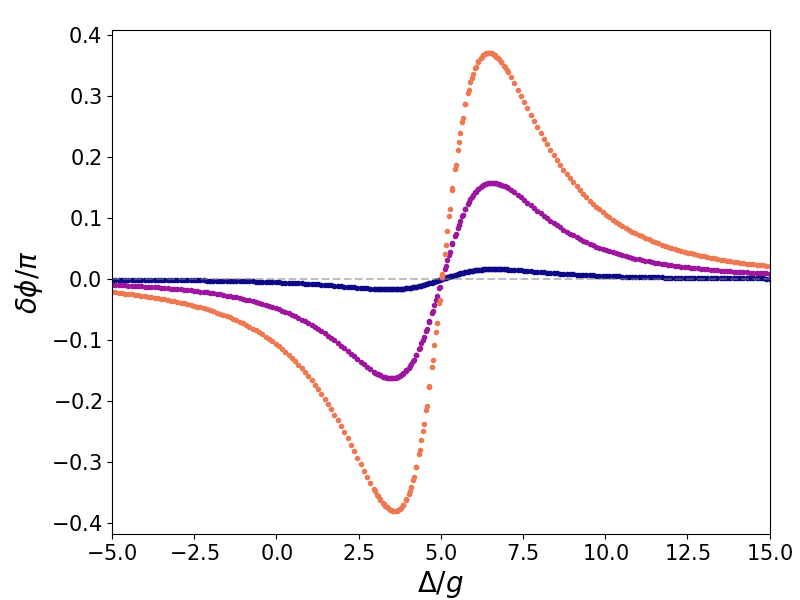
\includegraphics[width=\textwidth]{figuras/ch5/robustez/delta/eg0+ge0 k=0.0g x=5.0g J=0.0g.png}
        \caption{}
        \label{fig5:robustez detunning 2 eg0}
    \end{subfigure}
    \vfill

    \caption{Robustez en funcion de $\Delta$ para la condición inicial $\frac{1}{\sqrt{2}}(\ket{eg0}+\ket{ge0})$ para (a) $\chi=0$ y (b) $\chi=5g$.}
    \label{fig5:robustez detunning eg0}
\end{figure}

En este gráfico se muestran tres curvas diferentes correspondientes a tres valores diferentes del acoplamiento con el entorno, respectivamente caracterizados por $\gamma=0.01g,0.1g$ y $0.25g$, y la condición inicial $\frac{1}{\sqrt{2}}(\ket{eg0}+\ket{ge0})$. En primer lugar, se ve que las curvas pasan por el origen, lo que nos dice que la diferencia entre la fase geométrica en ambos casos es 0, que es lo que llamamos condición de robustez, ya que el entorno no tiene efecto sobre la fase geométrica y esta se mantiene robusta ante los efectos del entorno. En el panel \ref{fig5:robustez detunning 1 eg0}, correspondiente a $\chi=k-J=0$, la condición de robustez se da para $\Delta=0$, como era de esperarse, ya que es la misma que para el caso de 1 átomo. De la misma manera, al observar el caso de $\chi=5g$ en la figura \ref{fig5:robustez detunning 2 eg0}, esta condición se da para $\Delta=\chi=5g$, que también es lo que se espera.
\begin{figure}[h]
    \centering
    \begin{subfigure}{0.49\textwidth}
        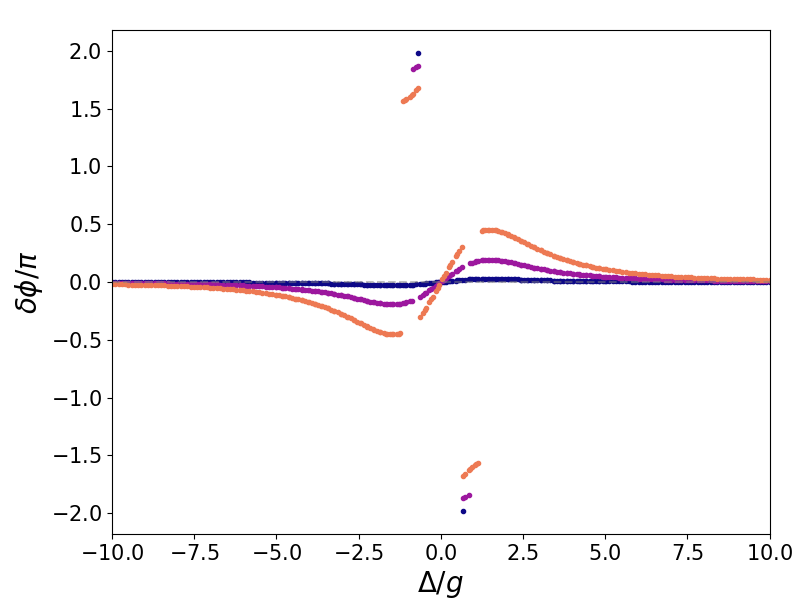
\includegraphics[width=\textwidth]{figuras/ch5/robustez/delta/eg1+ge1 k=0.0g x=0.0g J=0.0g.png}
        \caption{}
        \label{fig5:robustez detunning 1 eg1}
    \end{subfigure}
    \hfill
    \begin{subfigure}{0.49\textwidth}
        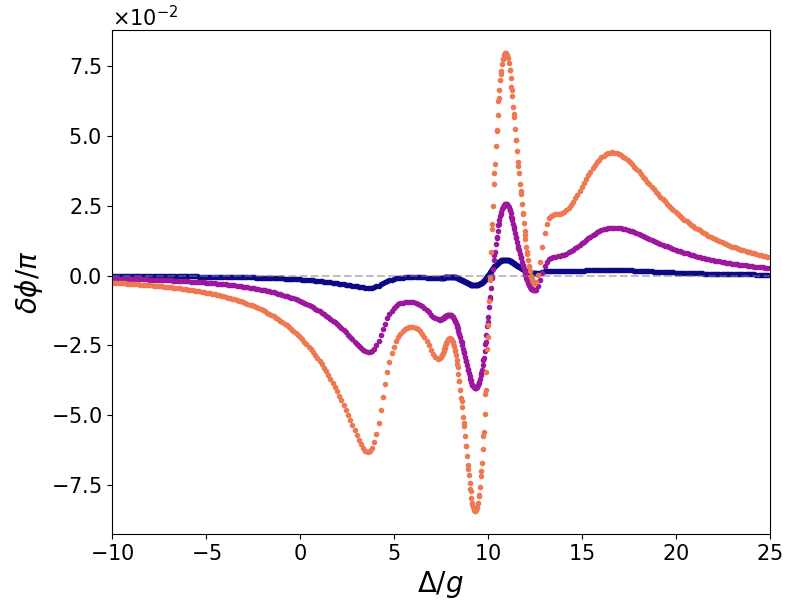
\includegraphics[width=\textwidth]{figuras/ch5/robustez/delta/eg1+ge1 k=0.0g x=5.0g J=0.0g.png}
        \caption{}
        \label{fig5:robustez detunning 2 eg1}
    \end{subfigure}
    \caption{Robustez en función de $\Delta$ para la condición inicial $\frac{1}{\sqrt{2}}(\ket{eg1}+\ket{ge1})$ para (a) $\chi=0$ y (b) $\chi=5g$}
    \label{fig5:robustez detunning eg1}
\end{figure}
La figura \ref{fig5:robustez detunning eg1} muestra la robustez para el estado inicial $\frac{1}{\sqrt{2}}(\ket{eg1}+\ket{ge1})$, sin interacción entre átomos, y para (\ref{sub@fig5:robustez detunning 1 eg1}) $\chi=0$ y (\ref{sub@fig5:robustez detunning 2 eg1}) $\chi=5g$. Con $\chi=0$, no cambia nada con respecto al caso de $N=1$. Pero cuando $\chi=5g$ se observan comportamientos nuevos: (i) hay máximos y mínimos nuevos que dependen suavemente de los parámetros y (ii) hay más de un valor para el cual la diferencia es 0 que además (iii) las condiciones de robustez no predicen correctamente. Para $\Delta=10g$ hay un punto de robustez, correspondiente a la condición dada por Ec. (\ref{ec4:condicion 3}) $\Delta=2\chi$, donde las tres curvas presentan una raíz. Pero también para $\Delta \approx 12.5g$ se observan otras raíces. El mínimo en esta zona depende del acoplamiento con el entorno, y sorprendentemente, para valores de $\gamma=0.1g$ y $\gamma=0.25g$, hay dos raíces, mientras que para $\gamma=0.01g$ no. Si bien las condiciones propuestas logran predecir el caso de robustez, es evidente que el efecto del entorno no se está teniendo en cuenta y puede llevar a comportamientos inesperados. Las dos evidencias más concretas de esto es que, por un lado, la condición de robustez predice correctamente pero con un muy pequeño error ocasionado por el corrimiento de frecuencias por el entorno, y por el otro lado, como se observó en este caso, hay algunos ceros nuevos de la función que aparecen al cambiar el acoplamiento con el entorno. Estos ceros no son condiciones de robustez, ya que suceden \textit{accidentalmente}, en el sentido que justo en el tiempo que se está observando la diferencia, la FG unitaria y disipativa coinciden, pero no en todo tiempo.


\subsection{Dependencia con el medio Kerr}
%chi list=(0.0001*g,0.1*g,0.5*g,g,2*g,5*g)

En el caso de 1 átomo se observó que el efecto del medio sobre la fase es análoga al detunning, y en el caso de dos átomos, se observa en la figura \ref{fig5:dependencia kerr eg0} la condición inicial $\frac{1}{\sqrt{2}}(\ket{eg0}+\ket{ge0})$ que esto sigue siendo cierto para el subespacio de $N=1$. Pero en el caso de la figura \ref{fig5:dependencia kerr eg1} se muestra que el efecto sobre la condición inicial $\frac{1}{\sqrt{2}}(\ket{eg1}+\ket{ge1})$, en comparación con la figura \ref{fig5:dependencia detunning eg1}, muestra diferencias en el régimen intermedio que se había definido aproximadamente para valores entre $1g \leq \chi \leq 5g$. Si bien la forma no es igual, es notable que el rango que se definió como \textit{intermedio} es el mismo. Entonces, si bien para $N=2$ el medio Kerr no es simplemente un corrimiento en el detunning, el comportamiento es similar. 

\begin{figure}[h]
    \centering
    \begin{subfigure}{0.49\textwidth}
        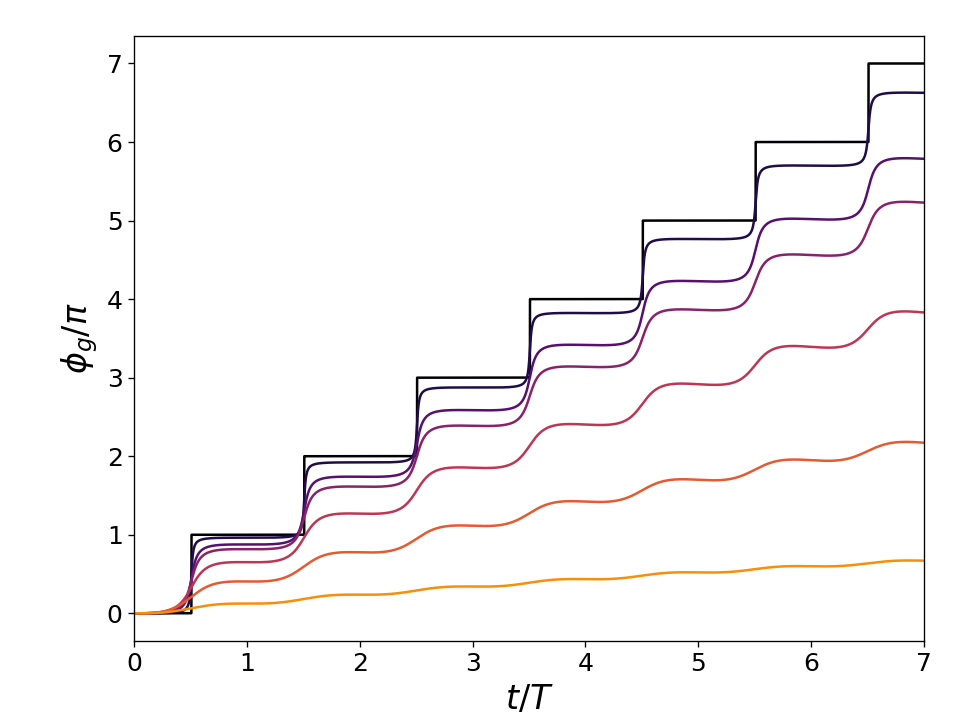
\includegraphics[width=\textwidth]{figuras/ch5/dependencia/eg0+/kerr todo 0.png}
        \caption{}
        \label{fig5:dependencia kerr eg0}
    \end{subfigure}
    \hfill
    \begin{subfigure}{0.49\textwidth}
        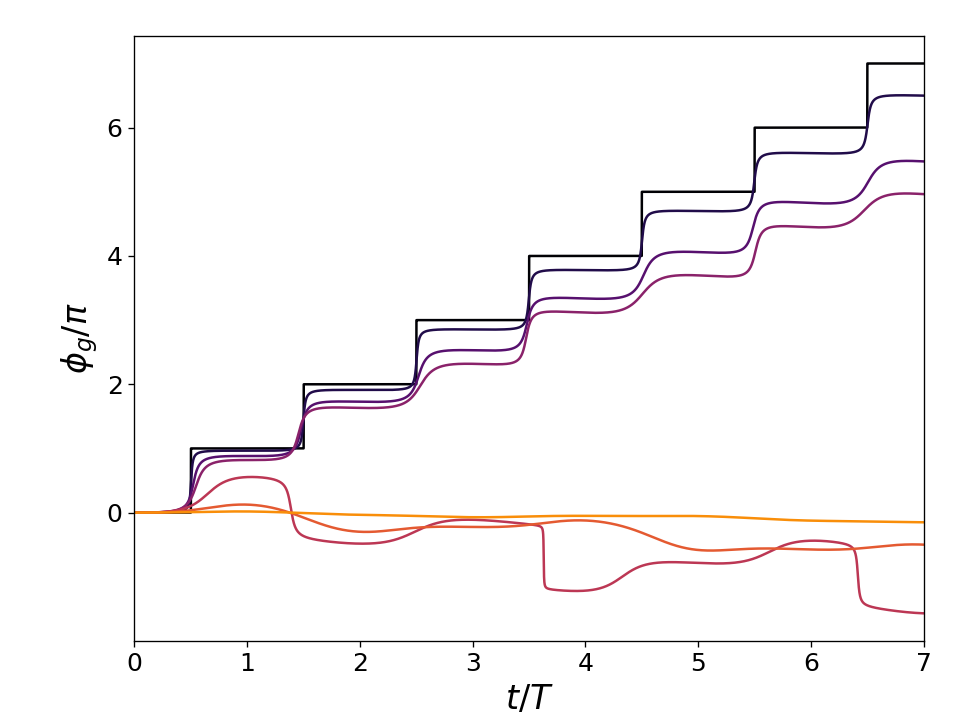
\includegraphics[width=\textwidth]{figuras/ch5/dependencia/eg1+/kerr todo 0.png}
        \caption{}
        \label{fig5:dependencia kerr eg1}
    \end{subfigure}
    \caption{Dependencia de la FG acumulada con el medio Kerr para condiciones iniciales (a) $\frac{1}{\sqrt{2}}(\ket{eg0}+\ket{ge0})$ y (b) $\frac{1}{\sqrt{2}}(\ket{eg1}+\ket{ge1})$.}
    \label{fig5:dependencia kerr}
\end{figure}

La pregunta que surge de todas formas es, qué sucede si se realiza un corrimiento en el detunning. En el caso de 1 átomo se había observado cómo la condición de robustez se cumplía cuando $\Delta=\chi(2n-1)$, y la dependencia de la fase geométrica parecía no cambiar, solo presentaba un corrimiento. 

En la figura \ref{fig5:dependencia kerr 2 eg0} se observa cómo en el primer caso, aumentar el detunning hace que las primeras cuatro curvas, que representan valores de $\chi=0,\;g/10,\;g/6\; y\;g/4$ (en negro y violeta oscuro respectivamente), acumulan fase negativa y los saltos son suaves. Ahora, la curva de $\chi=\Delta=0.5g$ (línea violeta claro) es igual a la de $\chi=\Delta=0$ de la figura \ref{fig5:dependencia kerr eg0}, y a partir de esta, al seguir aumentando el detunning el comportamiento es el mismo que antes. Pero para el caso de $N=2$, ya no es así. Primero, para $\chi=0$ y $\chi=0.1g$ las curvas presentan saltos más abruptos, y hay un rebote. Por otro lado, el caso robusto ya no se observa para $\chi=0.5g$. Ahora, la curva violeta oscura, que representa un valor de $\chi=\frac{\Delta}{3}=g/6$, si bien no es el caso robusto, es muy similar. Se probó por inspección y el valor encontrado para la robustez se dio para $\chi=0.37\Delta$. Esto coincide aproximadamente con la condición de la Ec. (\ref{ec4:condicion 3}). Si se sigue aumentando el valor de $\chi$, en el rango intermedio las oscilaciones de la fase parecen tener más de una componente en frecuencia. Esto se observa claramente en la curva roja, donde se ve que hay dos saltos diferentes. 

\begin{figure}[h]
    \centering
    \begin{subfigure}{0.49\textwidth}
        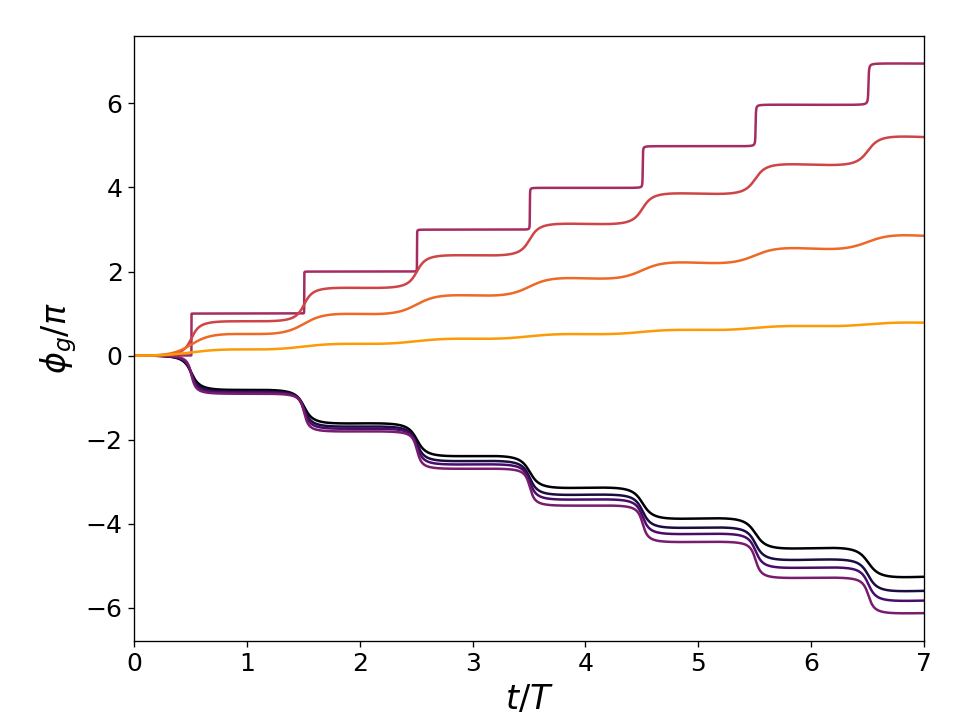
\includegraphics[width=\textwidth]{figuras/ch5/dependencia/eg0+/ker d=0.5g.png}
        \caption{}
        \label{fig5:dependencia kerr 2 eg0}
    \end{subfigure}
    \hfill
    \begin{subfigure}{0.49\textwidth}
        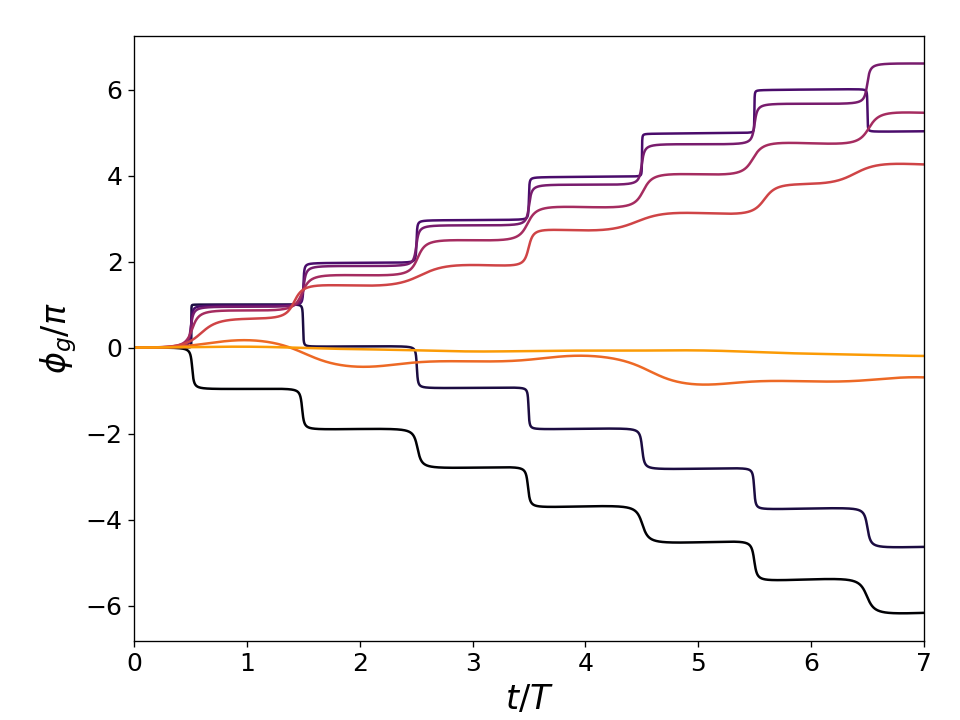
\includegraphics[width=\textwidth]{figuras/ch5/dependencia/eg1+/kerr d=0.5g.png}
        \caption{}
        \label{fig5:dependencia kerr 2 eg1}
    \end{subfigure}
    \caption{Dependencia de la FG acumulada con el medio Kerr con $\Delta=0.5g$ para condiciones iniciales (a) $\frac{1}{\sqrt{2}}(\ket{eg0}+\ket{ge0})$ y (b) $\frac{1}{\sqrt{2}}(\ket{eg1}+\ket{ge1})$.}
    \label{fig5:dependencia kerr 2}
\end{figure}

Finalmente, se realiza un gráfico de diferencias entre la FG unitaria y la disipativa en función del parámetro $\chi$. En la figura \ref{fig5:robustez kerr eg0} se muestra la diferencia $\delta\phi=\phi_d-\phi_u$ para la condición inicial $\frac{1}{\sqrt{2}}(\ket{eg0}+\ket{ge0})$. Se ve cómo la condición de robustez en este caso es igual que para el modelo de 1 átomo, donde la condición se da para $\Delta=\chi$. 

\begin{figure}[h]
    \centering
    \begin{subfigure}{0.49\textwidth}
        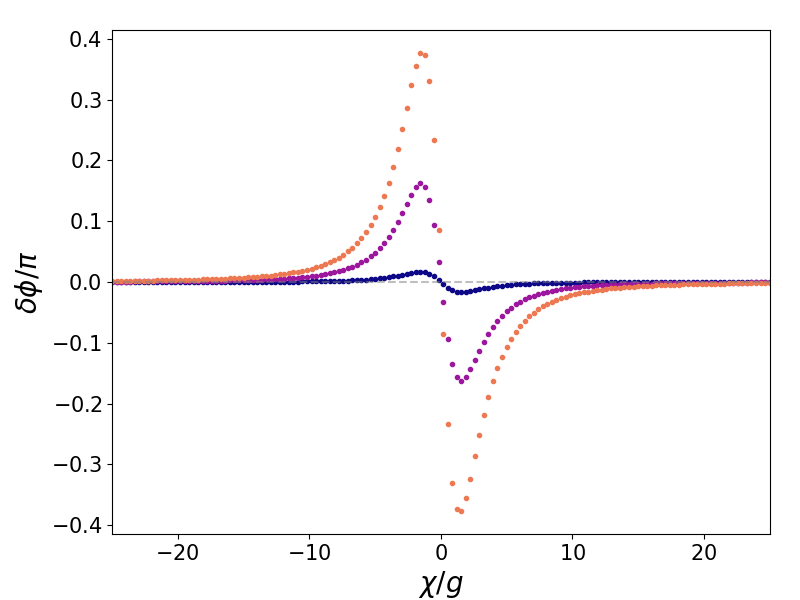
\includegraphics[width=\textwidth]{figuras/ch5/robustez/chi/eg0+ge0 d=0.0g k=0.0g J=0.0g.png}
        \caption{}
        \label{fig5:robustez kerr 1 eg0}
    \end{subfigure}
    \hfill
    \begin{subfigure}{0.49\textwidth}
        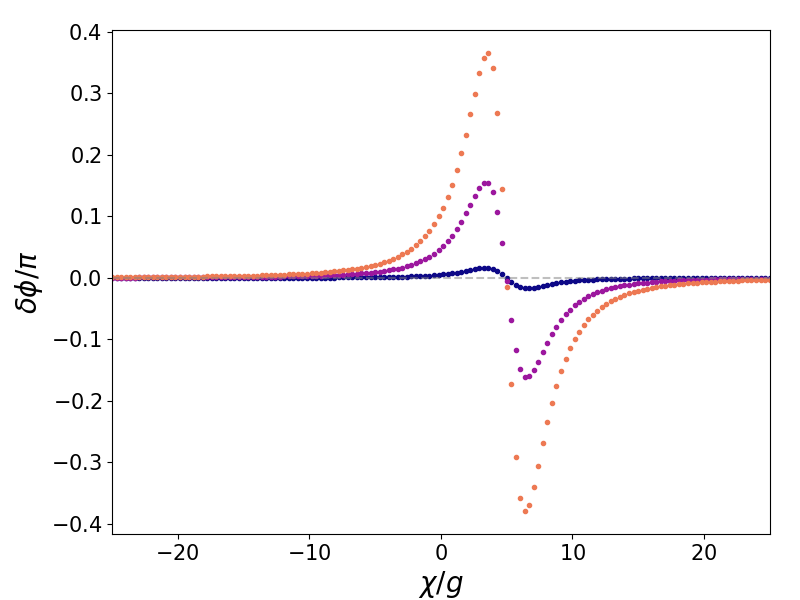
\includegraphics[width=\textwidth]{figuras/ch5/robustez/chi/eg0+ge0 d=5.0g k=0.0g J=0.0g.png}
        \caption{}
        \label{fig5:robustez kerr 2 eg0}
    \end{subfigure}
    \caption{Robustez en función de $\chi$ para la condición inicial $\frac{1}{\sqrt{2}}(\ket{eg0}+\ket{ge0})$ con (a) $\Delta=0$ y (b) $\Delta=5g$}
    \label{fig5:robustez kerr eg0}
\end{figure}

Para la condición inicial $\frac{1}{\sqrt{2}}(\ket{eg1}+\ket{ge1})$ se muestra la figura \ref{fig5:robustez kerr eg1}. Primero, en el panel (\ref{sub@fig5:robustez kerr 1 eg1}) se muestra el caso de $\Delta=0$. La única raíz se da para $\chi=\Delta=0$.

\begin{figure}[h]
    \centering
    \begin{subfigure}{0.49\textwidth}
        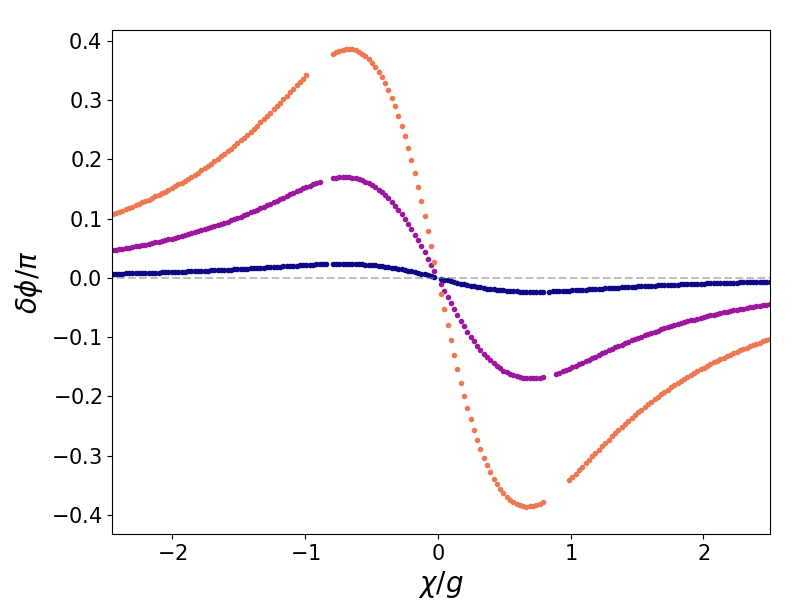
\includegraphics[width=\textwidth]{figuras/ch5/robustez/chi/eg1+ge1 chi zoom.png}
        \caption{}
        \label{fig5:robustez kerr 1 eg1}
    \end{subfigure}
    \hfill
    \begin{subfigure}{0.49\textwidth}
        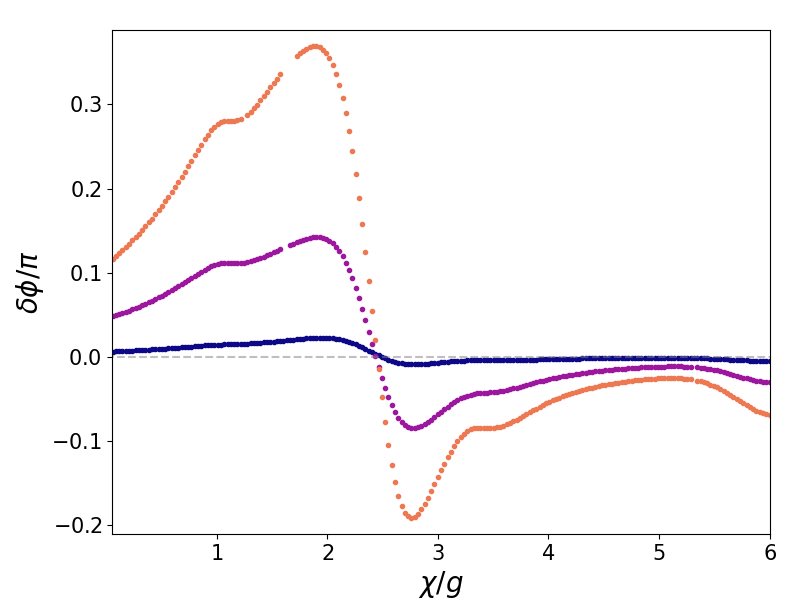
\includegraphics[width=\textwidth]{figuras/ch5/robustez/chi/eg1+ge1 chi d=5.0g.png}
        \caption{}
        \label{fig5:robustez kerr 2 eg1}
    \end{subfigure}
    \caption{Robustez en función de $\chi$ para la condición inicial $\frac{1}{\sqrt{2}}(\ket{eg1}+\ket{ge1})$ con $k-J=0$ y (a) $\Delta=0$; (b) $\Delta=5g$}
    \label{fig5:robustez kerr eg1}
\end{figure}

Hay que aclarar parte de las curvas donde no tienen puntos. En estos casos lo que sucede es que el entorno introduce un corrimiento en las frecuencias. Consecuentemente, hay un pequeño cambio entre la fase unitaria y la no unitaria. En principio, esto no es un problema, ya que lo único que hace es retrasar un poco el escalón. Pero en combinación con la dinámica complicada del sistema, lo que ocurre en casos muy puntuales, es que la fase unitaria y la disipativa hacen un escalón en direcciones contrarias y la diferencia entre ambas presenta un salto abrupto. En la figura \ref{fig5:robustez kerr 1 eg1} cerca de los valores $\chi/g=\pm 1$ se observan la falta de puntos, estos están más arriba por el salto que se mencionó. Es también interesante, que no es solo para un caso aislado, sino que es en un rango de valores donde se observa este comportamiento. 

En la figura \ref{fig5:robustez kerr 2 eg1} se muestra el caso en donde se aumentó el detunning hasta $\Delta=5g$. Se observan máximos y mínimos locales, y la condición de robustez parece estar cercana a $\chi\simeq 2.45g$ y varía suavemente con cada valor de $\gamma$. Esto es muy interesante, ya que el efecto que tiene el entorno también se refleja en esta condición. Nuevamente, esta condición en el subespacio de $N=2$ se da cuando $\Delta=2\chi$ (Ec. (\ref{ec4:condicion 3})), y en la figura \ref{fig4:concu x 1 d2} se observa que para $\chi\simeq2.5g$ también la concurrencia presenta una franja robusta. Algo interesante es que la franja observada en la concurrencia, no es de una gran amplitud, aun así, la fase geométrica presenta una raíz para este caso. Si bien esto es un indicio de que la fase geométrica y la concurrencia están relacionadas, es evidente que hay un mecanismo más fundamental que genera este comportamiento y que será motivo de estudio en el futuro.

\subsection{Dependencia con la interacción entre átomos}
Finalmente, se considera la dependencia en la interacción entre los átomos $k-J$. En la figura \ref{fig5:dependencia interaccion} nuevamente se muestran las dos condiciones iniciales (a) $\frac{1}{\sqrt{2}}(\ket{eg0}+\ket{ge0})$ y (b) $\frac{1}{\sqrt{2}}(\ket{eg1}+\ket{ge1})$. En ambos casos el comportamiento es el mismo. Al aumentar la interacción, la FG acumulada es menor y los saltos son más suaves. A diferencia con el detunning y con el medio, no se reconoce un rango intermedio para el cual el comportamiento sea diferente. 

\begin{figure}[h]
    \centering
    \begin{subfigure}{0.49\textwidth}
        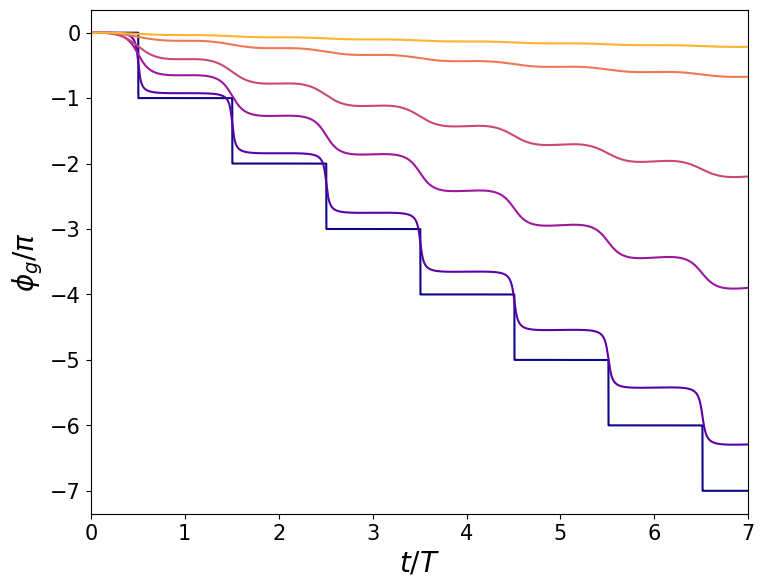
\includegraphics[width=\textwidth]{figuras/ch5/dependencia/eg0+/interaccion todo 0.png}
        \caption{}
        \label{fig5:dependencia interaccion eg0}
    \end{subfigure}
    \hfill
    \begin{subfigure}{0.49\textwidth}
        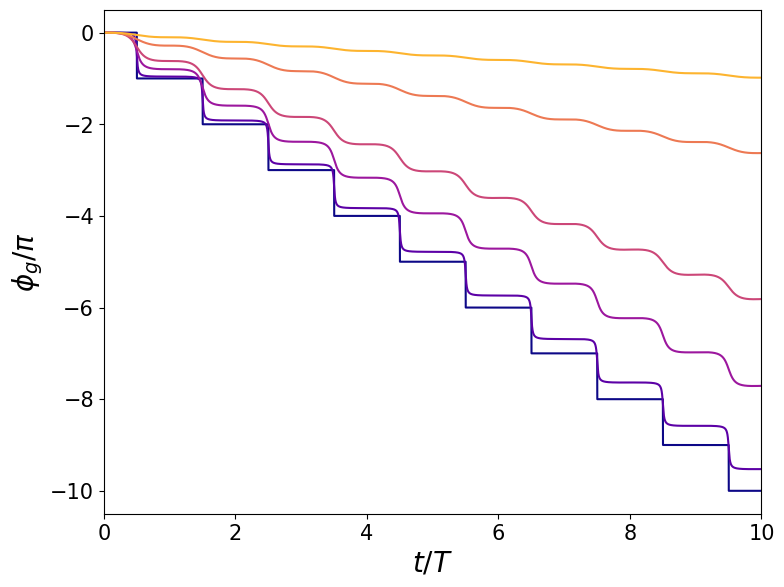
\includegraphics[width=\textwidth]{figuras/ch5/dependencia/eg1+/interaccion todo 0.png}
        \caption{}
        \label{fig5:dependencia interaccion eg1}
    \end{subfigure}
    \caption{Dependencia de la FG acumulada con la interacción entre los átomos $k-J$ para condiciones iniciales (a) $\frac{1}{\sqrt{2}}(\ket{eg0}+\ket{ge0})$ y (b) $\frac{1}{\sqrt{2}}(\ket{eg1}+\ket{ge1})$.}
    \label{fig5:dependencia interaccion}
\end{figure}
En la figura \ref{fig5:robustez interaccion eg0} se muestra la diferencia entre la FG unitaria y disipativa para la condición inicial $\frac{1}{\sqrt{2}}(\ket{eg0}+\ket{ge0})$. El comportamiento es el esperado: la condición de robustez se da cuando $k-J=\frac{\chi-\Delta}{2}$. Nuevamente, los máximos dependen suavemente de los parámetros, y en particular dependen del entorno $\gamma$. 
\begin{figure}[h]
    \centering
    \begin{subfigure}{0.49\textwidth}
        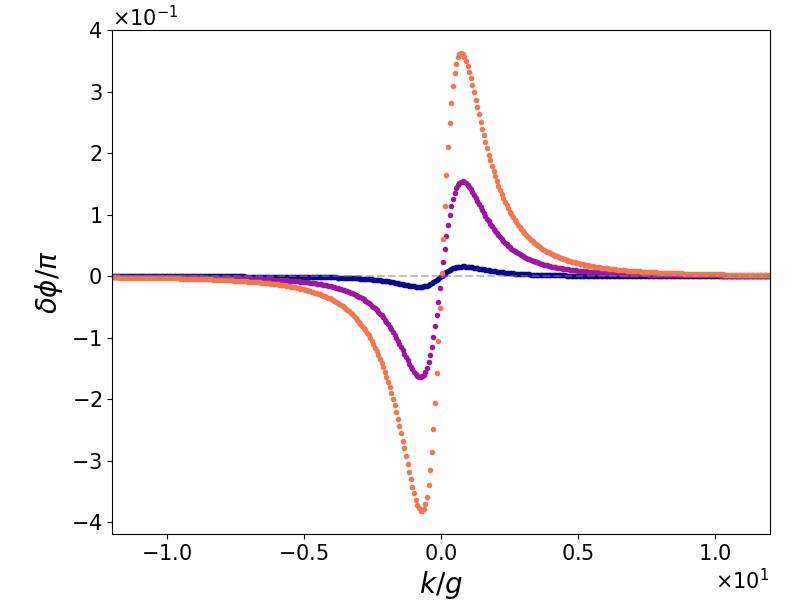
\includegraphics[width=\textwidth]{figuras/ch5/robustez/k/eg0+ge0 d=2.5g x=2.5g J=0.0g.png}
        \caption{}
        \label{fig5:robustez interaccion 1 eg0}
    \end{subfigure}
    \hfill
    \begin{subfigure}{0.49\textwidth}
        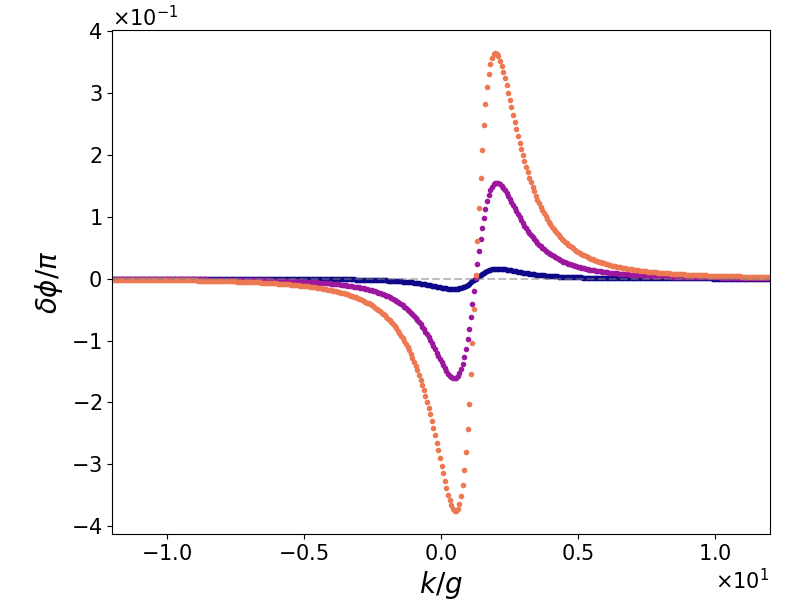
\includegraphics[width=\textwidth]{figuras/ch5/robustez/k/eg0+ge0 d=0.0g x=2.5g J=0.0g.png}
        \caption{}
        \label{fig5:robustez interaccion 2 eg0}
    \end{subfigure}
    \caption{Robustez en función de $\chi$ para la condición inicial $\frac{1}{\sqrt{2}}(\ket{eg0}+\ket{ge0})$ con $\Delta=0$ y (a) $\chi=0$; (b) $\chi=2.5g$}
    \label{fig5:robustez interaccion eg0}
\end{figure}

Para la condición inicial $\frac{1}{\sqrt{2}}(\ket{eg1}+\ket{ge1})$ se muestra la figura \ref{fig5:robustez interaccion eg1}. Cuando $\Delta=\chi=0$ (\ref{sub@fig5:robustez interaccion 1 eg0}), la dependencia parece ser la misma que en el caso de $\frac{1}{\sqrt{2}}(\ket{eg0}+\ket{ge0})$, pero en este caso la fase acumulada es menor por casi 1 orden de magnitud. 
\begin{figure}[h]
    \centering
    \begin{subfigure}{0.49\textwidth}
        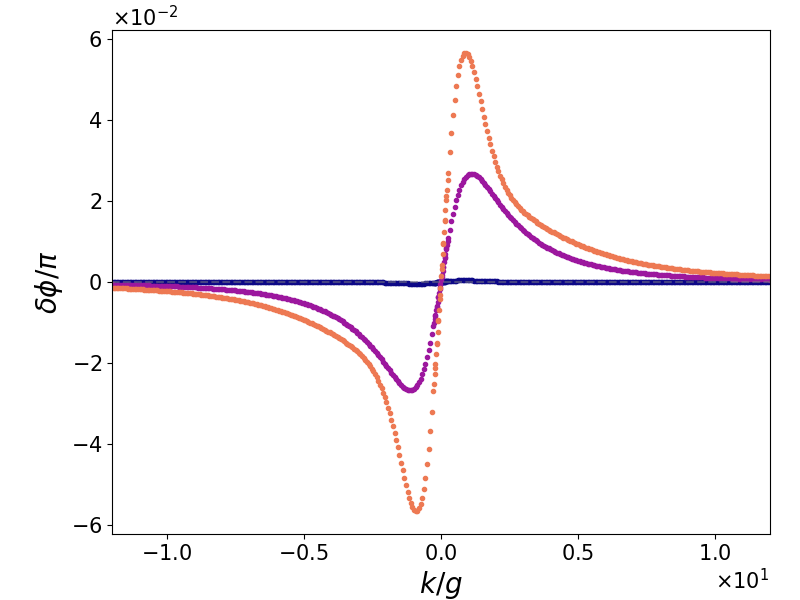
\includegraphics[width=\textwidth]{figuras/ch5/robustez/k/eg1+ge1 d=0.0g x=0.0g J=0.0g.png}
        \caption{}
        \label{fig5:robustez interaccion 1 eg1}
    \end{subfigure}
    \hfill
    \begin{subfigure}{0.49\textwidth}
        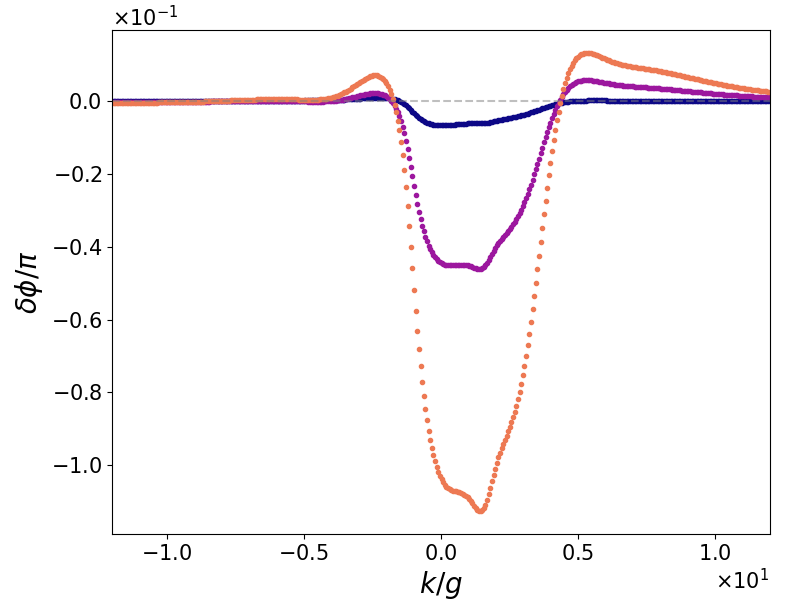
\includegraphics[width=\textwidth]{figuras/ch5/robustez/k/eg1+ge1 d=0.0g x=2.5g J=0.0g.png}
        \caption{}
        \label{fig5:robustez interaccion 2 eg1}
    \end{subfigure}
    \caption{Robustez en función de $\chi$ para la condición inicial $\frac{1}{\sqrt{2}}(\ket{eg1}+\ket{ge1})$ con $\Delta=0$ y (a) $\chi=0$; (b) $\chi=2.5g$}
    \label{fig5:robustez interaccion eg1}
\end{figure}
En la figura \ref{fig5:robustez interaccion 2 eg1} se muestra el caso en que $\Delta=0$ y $\chi=2.5g$. De las tres condiciones de robustez, la condición $\Delta-\chi(2n-2)$ (\ref{ec4:condicion 3}) no puede cumplirse nunca. 

Es interesante que en los casos estudiados anteriormente, en general, era esta la condición que predecía la condición de robustez. Como en este caso no es posible cumplir esta condición, entonces se ve que las otras dos condiciones actúan como condiciones de robustez, que se dan cuando $k-J=-\frac{\chi}{2}$ (Ec. (\ref{ec4:condicion 2})) y $k-J=\frac{3}{2}\chi$ (Ec. (\ref{ec4:condicion 1})). En este caso, en particular son para $k-J=-1.25g$ y $k-J=4.75g$, valores que se marcan con líneas rayadas. Si bien la predicción no es exacta, es bastante buena para aproximar. La discrepancia entre valor predicho y valor observado en las figuras se debe a que no se tuvo en cuenta el efecto del entorno a la hora de conseguir estas condiciones. Otra evidencia de esto es que el cero de cada una de las tres funciones, cuyos valores de $\gamma$ son diferentes, varían suavemente. 

\section{Robustez en función del detunning}

Finalmente, se explora más en detalle las condiciones de robustez dadas por las Ecs. (\ref{ec4:condicion 1})-(\ref{ec4:condicion 3}) en función del detunning. Esto es importante, ya que este es en general el parámetro de control al que se tiene acceso en los experimentos, en general, cambiando la frecuencia de la cavidad. 

Ya se vio que las condiciones de robustez (\ref{ec4:condicion 1})-(\ref{ec4:condicion 3}) predicen correctamente, con cierto error por el efecto del entorno, cuando la diferencia entre la FG unitaria y en sistema abierto es nula. Esto es uno de los resultados más importantes del trabajo, y se quiere estudiar si estas condiciones se cumplen en todos los casos, ya que si bien en los gráficos mostrados por ahora siempre se cumplió, no fueron demasiadas las combinaciones de parámetros estudiados. Lo que se va a hacer en esta sección, es realizar gráficos de robustez como se hicieron anteriormente, pero para un valor fijo del acoplamiento con el entorno $\gamma=0.25g$. También, ya que las condiciones de robustez que se encontraron salieron de pedir degeneración entre las energías de los estados de la base Ec. (\ref{ec4:base}), entonces se quiere ver qué pasa con las otras dos condiciones iniciales del subespacio de $N=2$, que son $\ket{gg2}$ y $\ket{ee0}$.

En la figura \ref{fig5:raices} se muestran los casos de robustez para las condiciones iniciales $\ket{gg2}$ mostradas con el número 1 en celeste, $\frac{1}{\sqrt{2}}(\ket{eg1}+\ket{ge1})$ con un número 2 en gris, y $\ket{ee0}$ con un número 3 en negro. Las tres líneas representan las tres condiciones de robustez (Ecs. (\ref{ec4:condicion 1})-(\ref{ec4:condicion 3}), para diferentes valores de $k-J$. En general, los casos robustos caen sobre las líneas predichas, y en su gran mayoría cada estado inicial respeta consistentemente alguna de las condiciones. Por ejemplo, los estados iniciales $\ket{gg2}$ y $\frac{1}{\sqrt{2}}(\ket{eg1}+\ket{ge1})$ respetan la condición $\Delta=2\chi$, y el estado inicial $\ket{ee0}$ respeta la condición de robustez $\Delta=\chi+2(k-J)$. Esto se cumple en la gran mayoría de los casos, pero como se observa en el caso de $k-J=2.5g$ (panel (c)), el estado inicial $\ket{gg2}$ en un principio respetaba la condición $\Delta=3\chi-2(k-J)$, pero luego este comportamiento cambió. 

Como se mencionó anteriormente, hay pequeñas discrepancias gracias al efecto del entorno. Para cuantificar estas diferencias, se realizó un ajuste lineal, y se obtiene que en presencia del entorno las condiciones se modifican un poco.
% \begin{figure}[h]
%     \centering
%     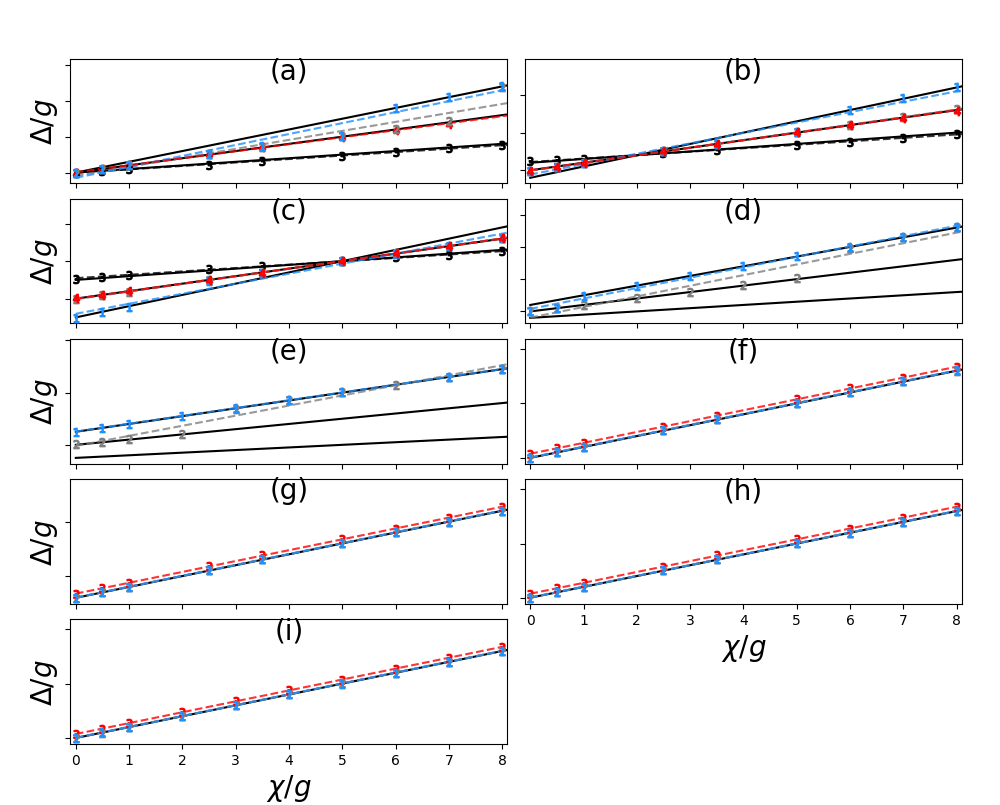
\includegraphics[width=\linewidth]{figuras/ch5/robustez/raices.png}
%     \caption{Condiciones de robustez para diferentes estados iniciales y valores de $k-J$. Los puntos representan las raíces de $\delta\phi_g=\phi_d-\phi_u$. Los paneles (a)-(e) son estados iniciales con 2 excitaciones, donde los colores representan el estado inicial: $\ket{gg2}$ en celeste, $\frac{1}{\sqrt{2}}(\ket{eg1}+\ket{ge1})$ en gris, $\ket{ee0}$ en negro y $\frac{1}{\sqrt{2}}(\ket{ee0}+{gg2})$ en rojo. En estas, los valores de $k-J$ son: (a) $k-J=0$, (b) $k-J=1g$, (c) $k-J=2.5g$, (d) $k-J=-1g$, (e) $k-J=-2.5g$. Las tres líneas negras son las condiciones de robustez predichas, donde la de mayor pendiente representa la condición Ec. (\ref{ec4:condicion 1}), la del medio Ec. (\ref{ec4:condicion 2}) y la de menor pendiente, la Ec. (\ref{ec4:condicion 3}). Los paneles (f)-(i) son para las condiciones iniciales de 1 excitación, donde está el $\ket{gg1}$ en celeste, $\frac{1}{\sqrt{2}}(\ket{eg0}+{ge0})$ en gris, y $\frac{1}{\sqrt{2}}(\frac{1}{\sqrt{2}}(\ket{eg0}+{ge0})+gg1)$ en rojo. La línea negra sólida representa la condición de robustez dada por Ec. \ref{ec4:condicion0}. Los valores de $k-J$ son: (f) $k-J=0$, (g) $k-J=1g$, (h) $k-J=2.5g$, (i) $k-J=-2.5g$.}
%     \label{fig5:raices}
% \end{figure}

El estado inicial $\ket{ee0}$ siempre sigue la condición Ec. (\ref{ec4:condicion 2}), y en presencia del entorno el ajuste predice una modificación aproximada según
\begin{equation}
    \Delta\simeq0.9\chi+2.2(k-J).
    \label{ec5:condicion 2 modificada}
\end{equation}
Los estados iniciales $\ket{gg2}$ y $\frac{1}{\sqrt{2}}(\ket{eg1}+\ket{ge1})$ siguen la condición (\ref{ec4:condicion 3}), y el ajuste en estos casos predice una condición modificada

\begin{equation}
    \Delta\simeq2.05\chi-0.05(k-J).
    \label{ec5:condicion 3 modificada}
\end{equation}
Similarmente, el estado inicial $\frac{1}{\sqrt{2}}(\ket{ee0}+\ket{gg2})$ también sigue la condición 2. Esto nos dice que los estados superposición de la base también siguen estas condiciones. Es interesante que, si bien el estado $\ket{gg2}$ a veces sigue la condición 1, y el $\ket{ee0}$ la 3, su superposición sigue la 2. Este estado es un estado entrelazado, solo si se mira el total del sistema. Si solamente se consideran los dos átomos, esto no es cierto, ya que la cavidad tiene diferente cantidad de excitaciones en cada estado, y por lo tanto al tomar traza parcial las coherencias desaparecen. 

Para los casos de 1 excitación, mostrados en las figuras \ref{fig5:raices}(f)-(i), se ve cómo las dos condiciones iniciales $\frac{1}{\sqrt{2}}(\ket{eg0}+\ket{ge0})$ y $\ket{gg1}$ siguen la única condición de robustez para este subespacio Ec. (\ref{ec3:condicion robuestez 1 atomo}). Sorprendentemente, cuando se considera el estado inicial entrelazado entre ambos estados de la base, $\frac{1}{\sqrt{2}}(\frac{1}{\sqrt{2}}(\ket{eg0}+\ket{ge0})+\ket{gg1})$, entonces presenta un pequeño \textit{offset} con respecto a los otros dos estados de la base. 
% \begin{figure}[h]
%     \centering
%     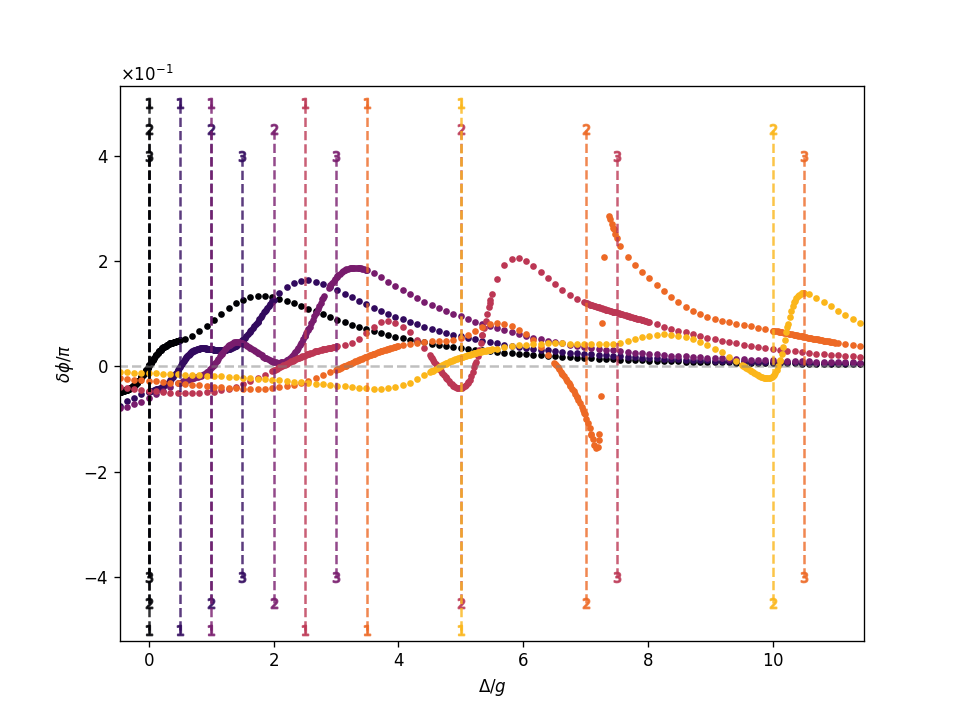
\includegraphics[ width=0.7\textwidth ]{figuras/ch5/robustez/ee0 k=0.0g J=0.0g delta-chi.png} 
%     \caption{Diferencia entre la FG unitaria y disipativa para $k-J=0$ y múltiples valores de $\chi\in [0,5g]$. Las líneas rayadas verticales representan las tres posibles condiciones de robustez.}
%     \label{fig5:inutil}
% \end{figure}



\section{Continuación del trabajo luego de presentar la tesis}

Lo primero que se revisó es si estas condiciones de robustez que se encontraron son correctas, y en el caso de ser correctas, si son exactas o aproximadas, y porque.

Lo primero entonces es revisar como se modifica la FG al cambiar los parámetros del sistema, y ver si la diferencia entre la FG unitaria y la FG en presencia de disipación son realmente iguales. Otra manera de mirar esto, es realizar el mismo estudio que antes, por ejemplo lo mostrado en la Figura \ref{fig5:inutil} para un tiempo más largo. 

Lo segundo que vamos a ver surge de la observación que, en el paper de Fer y Pau \cite{fg1}, el setup es parecido, tenemos dos átomos que interactúan con un campo bosonico. Entonces lo que vamos a ver es como se comporta la FG del modelo de TC (Tavis-Cummings), si realizamos una traza parcial sobre la cavidad. Esto es bastante interesante, ya que haciendo spoiler, la FG de los dos átomos da siempre cero. Esto se puede analizar por el tipo de interacción entre los átomos y la cavidad, que a diferencia del modelo de spin-boson, conserva la cantidad de excitaciones. Para el spin-boson tenemos el Hamiltoniano 

\begin{equation}
    H^{SB}=\frac{\hbar\Delta}{2}\sigma_z+\sigma_{j}\sum_n\lambda_nq_n+\sum_n\hbar\omega_na_n^\dagger a_n.
\end{equation}
Donde en general $j=z,x$. El primer caso es una situación con puro dephasing, y el segundo con relajación. También se puede hacer alguna combinación para obtener ambos afectos simultáneamente. Esto es para solo 1 átomo. En el paper \cite{fg1} tenemos un hamiltoniano muy parecido

\begin{align}
    H^{SB}_S=&\frac{\Omega_1}{2}\sigma_{z,1}+\frac{\Omega_2}{2}\sigma_{z,2}+\gamma\sigma_{z,1}\otimes\sigma_{z,2}, \\
    H^{SB}_I=&\sigma_{z,1}\otimes\sum_{n=1}^N\lambda_nq_n+\sigma_{z,2}\otimes\sum_{n=1}^Ng_nq_n, \\
    H^{SB}_B=\sum_{k=1}^N w_ka^\dagger_ka_k.
\end{align}

Se puede ver fácilmente, recordando que $q_n=q_{zpf}(a^\dagger_n+a_n)$, que la interacción qubits-entorno no conserva la cantidad de excitaciones. Una particularidad del modelo de SB (con 1 o 2 átomos) con puro dephasing, es que las coherencias son simplemente el valor inicial decayendo exponencialmente. No evolucionan oscilatoriamente ni se mezclan. Por lo tanto, si inicialmente no tenemos coherencias entre los átomos, tampoco las tendremos a $t>0$. Consecuentemente, la FG en este modelo, depende mucho de la condición inicial, y si no hay coherencias iniciales, entonces la FG sera nula $\forall t$. 

Por otro lado, en el modelo de TC, si consideramos a la cavidad como el entorno y una interacción entre átomos igual, que es lo que hice en la Tesis de Licenciatura, entonces tenemos

\begin{align}
    H^{TCM}_s=&\frac{w_1}{2}\sigma_{z,1}+\frac{w_2}{2}\sigma_{z,2}+J\sigma_{z,1}\sigma_{z,2}+2k(\sigma_{+,1}\sigma_{-,2}+\sigma_{-,1}\sigma_{+,2}), \\
    H^{TCM}_I=&\sum_{n=1}^N(\lambda_n\sigma_{+,1}+g_n\sigma_{+,2})a_n+\sum_{n=1}^N(\lambda_n\sigma_{-,1}+g_n\sigma_{-,2})a^\dagger_n, \\
    H^{TCM}_C=&\sum_{n=1}^Nw_na^\dagger_na_n.
\end{align}

Este Hamiltoniano si conserva la cantidad de excitaciones. Esto por parte es bueno, esto nos restringe el subespacio de Hilbert que es relevante para la evolución, pudiendo decir que entonces el Hamiltoniano se diagonaliza por bloques eligiendo correctamente la base, y por lo tanto la dinámica de la matriz densidad también sera diagonal por bloques, si tiene esta forma en su condición inicial. Esto es cierto si la evolución es unitaria. Pero se puede mostrar, que si la dinámica es disipativa, y utilizamos una ecuación maestra de tipo Linblad, entonces, de todas formas es cierto que la matriz densidad es diagonal por bloques a todo tiempo, si inicialmente lo es. Lo bueno de esto es que podemos resolver el problema (hasta cierto punto) analíticamente. El tipo de interacción nos restringe a un subespacio de 4x4, que a su vez se diagonaliza en un bloque de 3x3 y otro de 1x1, para cada suma de spin, que en este caso como tenemos dos qubits, el bloque de 3x3 representa al triplete, y el de 1x1 al singlete. Lo malo, es que si queremos mirar solo la dinámica de los dos qubits, trazando parcialmente sobre la cavidad, se puede ver con relativa facilidad que la matriz densidad reducida resultante, que es de 4x4 por ser de 2 qubits, es puramente diagonal, no presenta coherencias entre los estados. Esto es cierto siempre y cuando inicialmente, la matriz densidad total no tenga elementos no nulos fuera de la diagonal. A partir de ahora, asumimos que solo hay un modo en la cavidad.

Para ver que esto es cierto, basta con tomar un subespacio de 3x3 cualquiera, generado por la base $\{\ket{00,n},(\ket{01,n-1}+\ket{10,n-1})/\sqrt{2},\ket{11,n-2}\}$. Al tomar traza parcial sobre este subespacio, podemos pensar esta operación no unitaria como $\rho_r=\sum_n\bra{n}\rho_{tot}\ket{n}$, y es evidente que solamente sobrevivirán las poblaciones, y no las coherencias, por lo tanto la forma de la matriz densidad reducida será
\begin{equation}
    \rho_r(t)=\begin{pmatrix}
        c_1 & 0 & 0 & 0 \\
        0 & c_2 & 0 & 0 \\
        0 & 0 & c_3 & 0 \\
        0 & 0 & 0 & c_4 \\
    \end{pmatrix}.
\end{equation}
Como se mencionó en el párrafo anterior, esto no es cierto si la matriz densidad total inicialmente presenta coherencias fuera de los bloques diagonales. \textcolor{red}{MAL: Para que esto suceda, no hay otra manera que la matriz densidad inicial NO pueda escribirse como un producto $\rho_{tot}\neq\rho_r\otimes\rho_C$, donde $\rho_r\in\mathbb{C}^{4\times 4}$ y $\rho_C\in\mathbb{C}^{(N\times N)\otimes k}$. En el modelo de TC $k=1$. CORRECCIÓN: Esto esta mal porque en realidad estamos mirando en el bloque de cantidad de excitaciones. Entonces estamos buscando \"entrelazamiento entre estados de números de excitaciones diferentes\", y esto puede pasar aún cuando no están entrelazados los átomos con la cavidad. Ejemplo: $\frac{1}{2}(\ket{ee}+\ket{gg})\otimes(\ket{0}+\ket{1})$, este estado presenta estados fuera de la diagonal de bloques. Entonces lo correcto seria que el estado tiene que estar en una superposición pura de estados con diferente número de excitaciones.} 

Para visualizar esto, vamos a comparar como se comportan los elementos de matriz densidad total (átomos+cavidad) y reducida (solo átomos), y la FG para diferentes estados iniciales en la cavidad para los dos modelos, el spin-boson y el TCM. Consideraremos los casos en que el estado inicial un estado puro cuyo número de excitaciones está bien definido, también el caso en que la cavidad se encuentra en un estado térmico.

Para esto hice un montón de simulaciones. Mas o menos la conclusión es que la FG para el \textbf{TCM}, por un lado (bien hecho) es lo de la tesis si consideramos todo. Numéricamente, debería ser mejor aumentar el tamaño del espacio de Hilbert, pero según estas simulaciones se pierde la robustez de la FG al aumentar la dimensión. Si consideramos la traza sobre la cavidad, y miramos los dos espines, la FG da cero, porque los subespacio de N excitaciones que diagonaliza por bloque el Hamiltoniano de TC, la parte de la cavidad no tiene la misma cantidad de fotones, y por lo tanto al tomar traza parcial solo quedan las poblaciones, y no las coherencias, por lo tanto la FG de los espines es cero. 

Para el \textbf{TCM} los elementos de matriz evolucionan como esperábamos. Los bloques de 3x3 oscilan, y si agregamos disipación se va relajando y la amplitud de las poblaciones de los estados con mayor cantidad de excitaciones decae. Esto contribuye a la FG del sistema total, que unitariamente es efectivamente un problema de 3x3. Con disipación se complica y hay perturbaciones a la FG, principalmente en las subidas de los \textit{escalones} se notan diferencias. Las mesetas se mantienen aun en presencia de disipación durante un tiempo considerable. 

Pasando a considerar el modelo de \textbf{Spin-Spin-Boson}. En este modelo, recordando el paper de Fer y Pau, lo que pasa con las coherencias es que oscilan y decaen exponencialmente. Esto es un resultado teórico proveniente de la teoría de decoherencia y ecuaciones maestras. La amplitud de las oscilaciones está dada unicamente por las condiciones iniciales, por lo tanto, si inicialmente hay alguna coherencia que es nula, así lo será $\forall t$. Entonces para estudiar como funciona la FG del SSB hay que considerar un estado inicial que tenga coherencias no nulas, las cuales contribuirán a la FG hasta que estas decaigan. Si uno atribuye la FG al ángulo subtendido por la trayectoria en el espacio de fases, como el decaimiento es exponencial, este ángulo sigue \textit{vivo} aún a tiempos largos cuando el radio de la orbita tiene a 0 por el dephasing (mueren las coherencias y nos lleva dentro de la \textit{hiper}esfera de Bolch). Yá es sabido que estos modelos llevan a un estado asintótico mixto por culpa del decaimiento exponencial de las coherencias. 

Finalmente, el modelo de \textbf{RABI}. Al principio lo único que hice fue cambiar el termino de acoplamiento, donde cambie el de JC por un $\sigma_x(a+a^\dagger)$. El problema de esto es que no cambie los términos libres, y le deje como único termino el $\Delta\sigma_z$ del JC. Esto esta mal ya que el ultimo paso para llegar a este termino libre es una transformación unitaria que tiene un $\sigma_z$. En el modelo de JC esto lo único que hace shiftear el término libre para que se nos vaya la contribución del resonador, en cambio en el modelo de Rabi esta transformación unitaria no la podemos aplicar tan fácilmente ya que no conmutaría con el termino de interacción y entonces genera problemas. Por lo tanto, para realizar la comparación entre las dinámicas y/o las FG en el modelo de Rabi contra el modelo de TC, tenemos que deshacer este paso, y quedarnos con el Hamiltoniano anterior:
\begin{equation}
    H_R=\frac{\omega_q}{2}S_Z+\frac{\omega_r}{2}a^\dagger a+ gS_x(a+a^\dagger)
\end{equation}
y
\begin{equation}
     H_R=\frac{\omega_q}{2}S_Z+\frac{\omega_r}{2}a^\dagger a+ g(S_+a+S_-a^\dagger)
\end{equation}
donde $S_j=\frac{1}{2}\sum_i\sigma_j^{(i)}$ es el operador colectivo de spin ($j=x,y,x$) o de subida y bajada ($j=\pm$).

Las simulaciones muestran que ambas dinámicas son iguales mientras que se cumpla la RWA. El modelo funciona bien.

En resumen, el trabajo que realicé desde comienzo de 2025 hasta julio, fue intentar de encontrar razones para la robustez de la fase geométrica en el modelo de la tesis, un modelo de Tavis-Cummings, con relajación y dephasing. Primero ataque el problema lo mas formalmente posible, intentando de ir por la geometría del espacio de fases, y la estructura del grupo. No encontré una relación muy relevante como para poder explicar el problema desde ese lado. Algún paper de Perola Milman me llevo a pensar en esferas de Bloch en mas dimensiones, pero no hay una interpretación muy clara para este sistema, ya que en ese paper, lo que se encuentra es que se puede representar el espacio de estados como un producto de varias esferas, de $U(3)\otimes SU(2)$, aprovechando que podemos clasificar los estados por su entrelazamiento. Esto tiene una gran ventaja, y es que si el entrelazamiento entre ambos spines es máximo, y así se mantiene durante la evolución, podemos mapear la trayectoria en el espacio de estados a solo un $SU(2)$, permitiéndonos utilizar la esfera de Bloch. Lamentablemente, este no es el caso para este problema, pero aun así, me dio esperanzas para encarar desde el lado del entrelazamiento. Entonces me puse a estudiar un poco sobre entrelazamiento. 

En este problema, tenemos un entrelazamiento entre tres partes, es decir, multipartito. Lo que encontré es que cuando tenemos mas de 2 sistemas, el entrelazamiento ya no tiene una medida muy concreta que nos diga si un estado es máximamente entrelazado o no. Esto se debe a que hay diferentes clases de entrelazamiento multipartito. Por ejemplo, el estado $\ket{GHZ}=(\ket{000}+\ket{111})/\sqrt{2}$ es máximamente entrelazado en algún sentido, pero también lo es el estado $\ket{W}=(\ket{100}+\ket{010}+\ket{001})/\sqrt{3}$. Para estudiar entonces la relación entre el entrelazamiento y la robustez de la FG, hay que meterse por este terreno, donde hay incertezas y para mi no es algo tan claro. Implementar el entrelazamiento multipartito no tiene una definicion muy concreta, ya que no hay medidas de entrelazamiento multipartito que sean muy utiles. Por ejemplo, existe el 3-tangle que parece estar bueno, pero solo esta definido para un sistema de 3 qubits, no hay nada con qubit-qubit-boson que yo haya encontrado. Ademas, el 3-tangle se basa en entralazamientos residuales entre las partes. Lo que me parecio mas correcto al final del dia es la negatividad, creo que no es monotona para todos los estados, pero creo que en este caso es suficientemente buena.

Implemente la negatividad y tambien otra medida que es la entropia relativa de entrelazamiento, que se implementa computacionalmente con el convex roof extension. Es muy cara computacionalmente asi que me quedo con la negatividad. 


    \chapter{Decoherencia}
\label{ch4_decoherencia}


%CAMBIAR ESTO PARA PERSONALIZARLO A MI GUSTO
\pagestyle{fancy}
\fancyhf{}
\fancyhead[LE]{\nouppercase{\rightmark\hfill}}
\fancyhead[RO]{\nouppercase{\leftmark\hfill}}
\fancyfoot[LE,RO]{\hfill\thepage\hfill}

En este capitulo voy a poner algunas cuentas y deducciones que estén relacionadas a la decoherencia. Mi objetivo es encontrar modelos analíticos para describir la decohrencia en el modelo de Jaynes-Cummings/Tavis-Cummings y en particular comparar con el caso de 2 átomos en un entorno bosonico, por ejemplo en el paper de fer y pau \cite{fg1}, el curso dictado por J.P. Paz y Zurek sobre decoherencia \cite{CursoPazZurek1999}  y también el libro de Breuer y Petruccione \cite{Breuer2002}.

\section{Dynamics of quantum open systems: master equiations. Curso Paz y Zurek. Capitulo 3.}

En este capitulo presentan varias herramientas y métodos para obtener ecuaciones maestras. En particular se utilizan perturbaciones en el acoplamiento entre sistema y entorno hasta segundo orden para describir un esquema general que luego es aplicado a dos ejemplos interesantes: movimiento browniano de una partícula acoplada a un entorno de osciladores, y una partícula acoplada localmente a un campo escalar cuántico. 

\subsection{Ecuaciones maestras: evaluación perturbativa}
El Hamiltoniano a considerar es
$$H=H_S+H_\varepsilon+V$$
donde los primeros dos son los hamiltonianos libres del sistema y el entorno respectivamente, y $V$ es la interacción.
En el picture de interacción la ecuación para la matriz densidad es
$$i \hbar \dot{\tilde\rho} = [\tilde V(t),\tilde\rho_{tot}(t)] $$
donde el tilde nos dice que estamos en la representación de interacción $\tilde O(t) =U_0^\dagger O U_0 $. Resolvemos perturbativamente y nos sale la serie de Dyson
\begin{equation}
    \tilde\rho_{tot}=\sum_{n\geq1}\int_0^tdt_1\dots\int_0^{t_{n-1}}dt_n(\frac{1}{i\hbar})^n[\tilde V(t_1),\dots,[\tilde V(t_n),\tilde\rho_{tot}(0)]]
\end{equation}
Si nos quedamos a segundo orden, entonces obtenemos
\begin{equation}
    \dot{\tilde\rho}(t)=\frac{1}{i\hbar}Tr_\varepsilon[\tilde V(t),\rho_{tot}(0)]-\frac{1}{\hbar^2}\int_0^tdt_1Tr_\varepsilon[\tilde V(t),[\tilde V(t_1),\rho_{tot}(0)]]
\end{equation}
Si suponemos que inicialmente el estado entre sistema y entorno no esta entrelazado, entonces $\rho_{tot}(0)=\rho(0)\otimes\rho_\varepsilon(0)$
\begin{equation}
      \dot{\tilde\rho}(t)=\frac{1}{i\hbar}Tr_\varepsilon[\tilde V(t),\rho(0)\otimes\rho_\varepsilon(0)]-\frac{1}{\hbar^2}\int_0^tdt_1Tr_\varepsilon[\tilde V(t),[\tilde V(t_1),\rho(0)\otimes\rho_\varepsilon(0)]]
\end{equation}
Lo que necesitamos ahora es que esto quede en función de la matriz densidad a tiempo $t$. Para eso la observación es que podemos escribir el $\rho(0)$ en función de $\tilde\rho(t)$ usando la misma expansión perturbativa que antes. Podemos entonces reescribir la ecuación como 

\begin{equation}
    \begin{split}
        \dot{\tilde\rho}(t)=&\frac{1}{i\hbar}Tr_\varepsilon[\tilde V(t),\tilde\rho\otimes\rho_\varepsilon(0)]-\frac{1}{\hbar^2}\int_0^tdt_1Tr_\varepsilon[\tilde V(t),[\tilde V(t_1),\rho\otimes\rho_\varepsilon]] \\ &+\frac{1}{\hbar^2}\int_0^tdt_1Tr_\varepsilon\left([\tilde V(t),Tr_\varepsilon([\tilde V(t_1),\tilde\rho\otimes\rho_\varepsilon])\otimes\rho_\varepsilon]\right)
    \end{split}
\end{equation}
Lo interesante es que solo hicimos dos suposiciones, que es valida la expansión hasta segundo orden en el acoplamiento con el entorno, y que el estado inicial no esta correlacionado.
\subsubsection{Ecuacion maestra perturbativa para un sistema de dos niveles acoplado a un baño térmico bosonico}
Si consideramos un sistema de dos niveles acoplado a un entorno bosonico térmico, entonces un modelo de interacción posible es el siguiente hamiltoniano, que es valido \textbf{bajo la aproximación RWA}:
\begin{equation}
    H=\frac{\hbar\Delta}{2}\sigma_z+\sum_n\lambda_n(a_n\sigma_++a^\dagger_n\sigma_-)+\sum_n\hbar\omega_na^\dagger_na_n
\end{equation}
Si seguimos con el procedimiento anterior, se obtiene la ecuación maestra en la picture de Schroedinger
\begin{equation}
    \begin{split}
        \dot\rho=&\frac{1}{i\hbar}[H_S,\rho] \\ & -\frac{1}{2\hbar^2}\int_0^tdt_1k(t_1)([\sigma_+,[\sigma_-(-t_1),\rho]]+[\sigma_+,\{\sigma_-(-t_1),\rho\}] + \text{h.c.})
    \end{split}
\end{equation}
donde el nucleo $k(t)$ esta definido como
\begin{equation}
    k(t)=\sum_n\lambda_n^2\langle[a_n(t),a_n^\dagger]\rangle=\sum_n\lambda_n^2\exp(-i\omega_nt)
\end{equation}
Usando la solucion de las ecuaciones de Heisenberg libres para los operadores del spin, que son
$$\sigma_\pm(t)=\sigma_\pm\exp(\pm i\Delta t)$$
obtenemos
\coloredeq{eq:spin-sigmax}{\dot\rho=\frac{1}{i}[\frac{\Delta}{2}-c(t),\rho]+a(t)(\sigma_+\sigma_-\rho+\rho\sigma_+\sigma_--2\sigma_-\rho\sigma_+)}

con $a(t)=2\Re\{f(t)\}$, $c(t)=\Im\{f(t)\}$, $f(t)=\frac{1}{2\hbar^2}\int_0^tdsk(s)\exp(i\Delta s)$

\subsubsection{Ecuación maestra para spin-boson}
La diferencia entre este modelo y el anterior radica en el tipo de interacción. Este modelo tiene una interacción que no conserva la cantidad de excitaciones. El Hamiltoniano del spin-boson es
\begin{equation}
    H=\frac{\hbar\Delta}{2}\sigma_x+\sigma_z\sum_n\lambda_nq_n+\sum_n\hbar\omega_na_n^\dagger a_n
\end{equation}
donde $q_n$ son las coordenadas de los osciladores del entorno (bosones). La ecuación maestra es
\begin{equation}
    \dot\rho =\frac{1}{i\hbar}[H_S,\rho]-\frac{1}{\hbar}\int_0^tdt_1\left( \nu(t_1)[\sigma_z,[\sigma_z(-t_1),\rho]]-i\eta(t_1)[\sigma_z,\{\sigma_z(-t_1),\rho\}] \right)
\end{equation}
con los núcleos de ruido y de decoherencia dados respectivamente por
\begin{equation}
    \begin{aligned}
        \nu(t)=& \frac{1}{2\hbar}\sum_n\lambda_n^2\langle\{q_n(t),q_n(0)\}\rangle=\int_0^\infty d\omega J(\omega)\cos(\omega t)(1+2N(\omega))\\
        \eta(t) = & \frac{1}{2\hbar}\sum_n\lambda_n^2\langle[q_n(t),q_n(0)]\rangle=\int_0^\infty d\omega J(\omega)\sin(\omega t)
    \end{aligned}
\end{equation}
con la densidad espectral $J(\omega)=\sum_n\lambda_n^2\delta(\omega-\omega_n)/2m_n\omega_n$ y también recordemos que $N(\omega)$ es el numero de ocupación de Boltzmann,  y por lo tanto $1+2N(\omega)=\coth(\beta\hbar\omega/2)$
Usando las ecuaciones libre de Heisenberg $\sigma_z(t)=\sigma_z\cos(\Delta t)+\sigma_y\sin(\Delta t)$, entonces obtenemos
\coloredeq{eq:spin-boson}{\frac{1}{i\hbar}[H_{eff},\rho]-\tilde D(t)[\sigma_z,[\sigma_z,\rho]]+z(t)\sigma_z\rho\sigma_y+z^*(t)\sigma_y\rho\sigma_z }
donde tenemos un Hamiltoniano efectivo y coeficientes dependientes del tiempo
\begin{equation}
    \begin{aligned}
        H_{eff}=&\hbar\left(\frac{\Delta}{2}-z^*(t)\right)\sigma_x \\
        \tilde D(t) =&\int_0^tds\;\nu(s)\cos(\Delta s) \\
        z(t) = & \int_0^tds\;(\nu(s)-i\eta(s))\sin\Delta s
    \end{aligned}
\end{equation}

\subsubsection{Ecuación maestra para una partícula interactuando con un quantum field}
\textit{Esto creo que puede servir para pensar en una linea de transmisión en el limite continuo, ya que en ese caso creo que tenemos un campo}
El sistema a considerar es una partícula con posición $\vec{x}$ y el entorno es un campo escalar $\phi$. La interacción es local, descrita por el termino $V=e\phi(\vec x)$, donde $e$ es la constante de acoplamiento (lo podemos pensar como la carga de la partícula). Expandiendo el campo en modos normales, la interacción la podemos escribir como
$$V=\int d\vec k (h_{\vec k}\exp(i\vec k \vec x) + \text{h.c.})$$ donde los $h_{\vec k}$ son proporcionales a los operadores de creación y destrucción:
$$h_{\vec k} = e a_{\vec k} /(2\pi)^{1/2}(2\omega_k)^{1/2}$$.
Es interesante notar que estamos haciendo un tratamiento puntual de la partícula, ya que la interacción es totalmente local. Esto sera consistente solo si intentamos de localizar a la partícula por fuera de la longitud de onda de Compton, de otra manera, necesitaríamos un tratamiento relativista donde tenemos en cuenta una interacción no local porque necesitamos tener en cuenta la extensión de la partícula. Se puede ver que el efecto de considerar una interacción no local es que al final, vamos a tener un cutoff dado por la longitud de onda de compton, la partícula no interactúa con modos cuyas frecuencias sean mayores que la masa en reposo de esta.

Asumiendo que el campo esta en equilibrio térmico, podemos obtener la ecuacion maestra para la partícula:
\begin{equation}
\begin{split}
    \dot \rho =  -\frac{i}{\hbar}[H,\rho]-\frac{e^2}{\hbar^2}\int d\vec k \int_0^t dt_1&\bigg(G_H(\vec k,t_1)[e^{i\vec k \vec x},[e^{-i\vec k \vec x(-t_1)},\rho]] -\\ & iG_R(\vec k,t_1)[e^{i\vec k \vec x},\{e^{-i\vec k \vec x(-t_1)},\rho\}]\bigg).
\end{split}
\end{equation}
donde $\vec x(t)$ es el operador de Heisenberg para la posición de la partícula (evolucionado con el H libre) y $G_{R,H}(\vec k,t)$ son las transformadas de Fourier de la función de dos puntos retardada y simétrica del campo escalar. Cuando el entorno es un campo libre tenemos
\begin{equation}
\begin{aligned}
    G_R(\vec{k},t) = & W(\vec k)\sin(\omega_{\vec k} t)/2\omega_{\vec k} \\
    G_H(\vec{k},t) = & W(\vec k)\cos(\omega_{\vec k} t)(1+2N(\omega))/2\omega_{\vec k} 
\end{aligned}    
\end{equation}
                                                                                                                                                                                                                                                                                                                                                                                                                                                                              
    \chapter{cQED}
\label{ch5_cqed}

\newcommand{\bop}{\hat{b}}
\newcommand{\bdag}{\hat{b}^\dagger}
\newcommand{\bdagT}{\hat{b}^{\dagger 2}}
\newcommand{\aop}{\hat{a}}
\newcommand{\adag}{\hat{a}^\dagger}
\newcommand{\adagT}{\hat{a}^{\dagger 2}}
\newcommand{\adagTh}{\hat{a}^{\dagger 3}}
\newcommand{\adagn}{\hat{a}^{\dagger n}}
\newcommand{\sigP}{\hat{\sigma}_+}
\newcommand{\sigM}{\hat{\sigma}_-}
\newcommand{\sigZ}{\hat{\sigma}_z}
\newcommand{\sigX}{\hat{\sigma}_x}
\newcommand{\sigY}{\hat{\sigma}_y}

%CAMBIAR ESTO PARA PERSONALIZARLO A MI GUSTO
\pagestyle{fancy}
\fancyhf{}
\fancyhead[LE]{\nouppercase{\rightmark\hfill}}
\fancyhead[RO]{\nouppercase{\leftmark\hfill}}
\fancyfoot[LE,RO]{\hfill\thepage\hfill}

Vamos a hablar de papers y algunos trabajos de circuitQED.

\section{Driven Multiphoton Qubit-Resonator Interactions}
Paper para final de la materia cQED.
\section{Introduction}
In the last century, mastering the manipulation of quantum-mechanical light-matter interactions emerged as a groundbreaking achievement. Today, the focus has evolved towards the precise engineering of versatile interactions, resilient to decoherence and practical imperfections, essential for advancing quantum technologies. This pursuit has the potential to advance information processing and error correction, and ultimately, it could lead to the realization of fault-tolerant quantum computing. Moreover, the precise control of light-matter interactions extends far beyond computing, finding diverse applications in quantum metrology, communication, and simulations, highlighting its profound impact across various domains.

The elementary model of quantum light-matter interactions is captured by the Rabi model where a qubit is linearly coupled to a single quantized field mode or a resonator \cite{}. This model describes the basic physics underlying most quantum computing implementations. This includes circuit quantum electrodynamics (QED) \cite{}, trapped ions \cite{}, and cavity QED \cite{}.

Different variants of the Rabi model exhibit a variety of higher order perturbative multiphoton effects stemming from a linear interaction (see for example Refs.).  These multiphoton perturbative effects have proven their utility in various applications, e.g. improved readout due to qubit-induced nonlinearity. Thus, to further control and leverage multiphoton effects, the Rabi model can be generalized to include nonlinear interactions, namely, a qubit nonlinearly coupled to a resonator through an $n$-photon interaction. These nonlinear models are nonperturbative, as the nonlinear interaction is inherent to the Hamiltonian rather than higher-order effects of a linear interaction term. Some of the spectral and dynamical properties of multiphoton Rabi models describing such nonlinear interactions, e.g. two-photon interactions, have been previously studied . Other studies of these models were focused on multiphoton blockades , `Fock state filters' that effectively confine the dynamics to a finite-dimensional subspace, enhancement of collective multiqubit phenomena  and stabilization of nonclassical states for quantum error correction \cite{}. Towards the goal of experimental realization, a series of nonperturbative implementations of the two-photon Rabi model have been recently proposed in superconducting circuits \cite{} and trapped ions \cite{}.


Much remains to be discovered about the various regimes of nonperturbative multiphoton qubit-resonator interactions, particularly when the qubit or resonator is driven, since the driving alters these interactions. In this paper, we develop a general theory for driving-enhanced nonperturbative multiphoton interactions in a qubit-resonator system. In particular, we study a qubit nonlinearly coupled to a resonator through an $n$-photon Rabi interaction in the presence of a qubit drive. 

The paper is structured as follows: Sec.~\ref{sec:DrivenInt} lays out the formalism for the theory. Then, the driving regimes on- and off-resonance from the qubit and resonator are explored. The driving is found to generate qubit-conditional operations on the resonator. {Next, we use two-tone driving to engineer an effective $n$-photon Rabi model that is tunable to arbitrary coupling strengths, thereby performing a quantum simulation of the model.} In Sec.~\ref{sec:TwoPhApp}, we apply the developed theory to the case of $n=2$, where we discover a \textit{qubit-conditional squeezing} (QCS) process. The QCS protocol allows for the encoding of a qubit state in the superposition of orthogonally squeezed states in the resonator. {Then, we show the potential use of the QCS protocol in the phase estimation algorithm with bosonic systems. We describe how the generators of the QCS operation can be used to realize faster unitary synthesis on the joint qubit-resonator Hilbert space.} We discuss how these applications can be generalized for higher-order interactions. Section~\ref{sec:cQED} proposes an implementation scheme based on the transmon qubit which can host the required two-photon interaction for implementing the QCS protocols. Lastly, we summarize our findings and present an outlook in Sec.~\ref{sec:Conc}.


\section{Enhancing multiphoton interactions with cross-resonant driving}\label{sec:DrivenInt}

In this section, we develop the theory of driving-enhanced interactions that enables qubit-conditional resonator operations. We proceed by stating the system and drive Hamiltonians and applying the necessary transformations to simplify its time dependence. Once we arrive at a simplified effective Hamiltonian, using the dressed basis, we explore the dynamics and its implications. Then, we add a second drive to the qubit, with properly chosen values of the amplitude and frequency, to engineer an effective $n$-photon Rabi Hamiltoninian with tunable parameters allowing the access to arbitrary coupling regimes.

\subsection{System Hamiltonian}
We start by considering the driven $n$-photon Rabi model whose Hamiltonian reads
\begin{subequations}\label{eq:SysHam}
\begin{align}
    \hat{H}=\hat{H}_{n-\text{R}} + \hat{H}_d
\end{align}
where
\begin{align}
    \hat{H}_{n-R}=\frac{\hbar \omega_q}{2}\hat{\sigma}_z+ \hbar\omega_r \hat{a}^\dagger\hat{a} + \hbar g_n(\hat{\sigma}_+ + \hat{\sigma}_-)(\hat{a}^{\dagger n} + \hat{a}^n),
\end{align}
and
\begin{align}
    \hat{H}_d=\hbar\Omega \cos(\omega_d t)(\sigP + \sigM).
\end{align}
\end{subequations}
Here, $\hat{\sigma}_z=\dyad{e}-\dyad{g}$ describes the population difference between the excited energy state $\ket{e}$ and the ground state $\ket{g}$ of the qubit, $\hat{\sigma}_+=\dyad{e}{g}$ and $\hat{\sigma}_-=\hat{\sigma}_+^{\dagger}$ are raising and lowering operators of the qubit, $\hat{a}$ and $\hat{a}^\dagger$ are the annihilation and creation operators of the resonator, $\omega_q$ is the transition frequency of the qubit, $\omega_r$ is the resonance frequency of the resonator, $g_n$  is the $n$-photon coupling strength between the resonator and qubit, $\Omega$ is the strength of the driving field and $\omega_{\text{d}}$ is the driving frequency. 

We rewrite the Hamiltonian of Eq.~\eqref{eq:SysHam} in a particular rotating frame, accounting for the $n$-photon nature of the qubit-resonator interaction, by means of the unitary transformation $\hat{U}^{r,n}=\exp[-i\omega_{\text{d}}t(\hat{\sigma}_z/2 + \hat{a}^\dagger \hat{a}/n)]$,
\begin{align}\label{eq:FullRotFrameHam}
    \hat{H}^r =& \hat{U}^{r,n \dagger} \hat{H}\hat{U}^{r,n}+i\hbar \dot{\hat{U}}^{r,n \dagger}\hat{U}^{r,n}\nonumber\\ =&\frac{\hbar \Delta}{2}\hat{\sigma}_z + \hbar \delta_n\hat{a}^\dagger \hat{a} \nonumber\\&+ \hbar g_n\big(\hat{\sigma}_+\hat{a}^n + \hat{\sigma}_-\hat{a}^{\dagger n}\nonumber\\ &\,\,\,\,\,\,\,\,\,\,\,\,\,\,\,\,\,\,\,\,+ e^{i2\omega_d t}\sigP\adagn + e^{-i2\omega_d t} \sigM\aop\big)\nonumber\\& +\frac{\hbar\Omega}{2}(\sigP +\sigM +e^{i2\omega_d t}\sigP + e^{-i2\omega_d t}\sigM), 
\end{align}
where $\Delta=\omega_q -\omega_d$ and $\delta_n=\omega_r - \omega_d/n$. We may now simplify this Hamiltonian by imposing the rotating-wave approximation (RWA) condition,
    \begin{align}
        &\label{eq:RWA2}g_n, \,\Omega,\, \Delta,\,\delta_n \ll \omega_d.
    \end{align}
This condition is neccesary to eliminate the fast-oscillating counter-rotating interaction terms, $g_n(e^{+i2\omega_{\text{d}}t}\hat{\sigma}_+\adagn +e^{-i2\omega_{\text{d}}t}\hat{\sigma}_-\hat{a}^n)$, and counter-rotating driving terms, $\Omega(e^{+i2\omega_{\text{d}}t}\hat{\sigma}_+ +e^{-i2\omega_{\text{d}}t}\hat{\sigma}_-)/2$. Imposing these RWA conditions, the simplified Hamiltonian reads

\begin{align}\label{eq:SimplifiedRotFrameHam}
    \hat{H}^r_{\text{RWA}} =&\frac{\hbar \Delta}{2}\hat{\sigma}_z +\frac{\hbar \Omega}{2}\hat{\sigma}_x + \hbar \delta_n\hat{a}^\dagger \hat{a} \nonumber\\&+ \hbar g_n(\hat{\sigma}_+\hat{a}^n +\hat{\sigma}_-\hat{a}^{\dagger n}), 
\end{align}
where $\hat{\sigma}_x=\hat{\sigma}_++\hat{\sigma}_-$. This last Hamiltonian will serve as the basis for our study.


\subsection{Effective interaction\label{sec:EffectiveInt}}
The qubit-resonator interaction changes depending on the driving parameters. We now aim to investigate the dynamics within two driving regimes, focusing on how the drive affects the qubit-resonator interaction. To better understand the driving regime's effect on the interaction and further simplify the analytical calculations, we transform to the interaction picture using the unitary $\hat{U}^{(I)}=\exp[-i \hat{H}_0 t/\hbar]$, where $\hat{H}_0=\hbar\Delta \hat{\sigma}_z/2 + \hbar\Omega\hat{\sigma}_x/2 + \hbar \delta_n \hat{a}^\dagger \hat{a}$. The interaction picture Hamiltonian reads
\begin{align}\label{eq:IntPicHam}
     \hat{H}^{(I)} =& \hat{U}^{(I) \dagger} \hat{H}^r_{\text{RWA}}\hat{U}^{(I)}+i\hbar \dot{\hat{U}}^{(I) \dagger}\hat{U}^{(I)}\nonumber\\ =&\hbar g_n\bigg[ \frac{\sin(\theta)}{2}\left( \dyad{\overline{+}}-\dyad{\overline{-}}\right) \nonumber\\&+\cos^2\left(\frac{\theta}{2}\right)e^{i\varepsilon t}\dyad{\overline{+}}{\overline{-}}\nonumber\\ &-\sin^2\left(\frac{\theta}{2}\right)e^{-i\varepsilon t}\dyad{\overline{-}}{\overline{+}}\bigg] \hat{a}^n e^{-in\delta_n t} + \text{H.c.},
\end{align}
where we use the dressed states $\ket{\overline{+}}=\sin\left(\theta /2\right)\ket{{g}}+\cos\left(\theta /2\right)\ket{{e}}$ and $\ket{\overline{-}}=\cos\left(\theta /2\right)\ket{{g}}-\sin\left(\theta /2\right)\ket{{e}}$, $\varepsilon=\sqrt{\Omega^2 +\Delta^2}$ and $\theta=\arctan(\Omega/\Delta)$.

The Hamiltonian of Eq.~\eqref{eq:IntPicHam} reveals two distinct interactions taking place at different timescales. One of these interactions oscillates with $e^{\pm i \varepsilon t}$; as the driving strength, $\Omega$, increases, these terms oscillate rapidly. We can eliminate these fast-oscillating terms by imposing the driving-detuning RWA condition \begin{align}\label{eq:DrivCond}
    |n\delta_n|,g_n\ll \varepsilon.
\end{align}
Imposing this condition allows us to obtain the effective Hamiltonian
\begin{align}\label{eq:EffHam}
\hat{H}^{(I)}_{\text{eff}}=\hbar \overline{g}_n (\dyad{\overline{+}}-\dyad{\overline{-}})(\hat{a}^{\dagger n} e^{ni\delta_n t}+\hat{a}^n e^{-ni\delta_n t}),
\end{align}
where $\overline{g}_n=g_n\sin(\theta)/2.$
The dynamics associated with this Hamiltonian result in a conditional $n$-photon {resonator operation dependent on the qubit state}. { The time-evolution operator generated by Eq.~\eqref{eq:EffHam} is \begin{align}\label{eq:GenTimeEvOp}
\hat{U}_{\text{eff},n}(t,0)=\dyad{\overline{+}}\hat{S}_n(\lambda(t)) + \dyad{\overline{-}}\hat{S}_n(-\lambda(t)), 
\end{align}
where $\hat{S}_n(\lambda)=\exp((\lambda^* \aop^n - 
\lambda \adagn)/n! )$ is the generalized $n$-photon squeezing operator \cite{GeneralizedSqueezing}; for $n=1$ it is the usual displacement operator, for $n=2$ it is the squeezing operator, etc., and $\lambda(t)=\overline{g}_n n! (e^{in \delta_n t}-1)/2n\delta_n $ is the generalized $n$-photon squeezing parameter.}

The driving-detuning condition can be achieved by changing $\Omega$ and $\Delta$ such that Eq.~\eqref{eq:DrivCond} is satisfied. The dressed basis states also depend on $\Omega$ and $\Delta$, and depending on the parameter regime, they can be approximated as the $\sigX$ or $\sigZ$ bases. In what follows, we explore the two extremes of strong driving and qubit-detuned weak driving. 
\subsubsection{Strong driving regime}\label{sec:StrongDriv}
When the driving is strong, $\Omega \gg \Delta$, $\ket{\overline{\pm}}\simeq\ket{\pm}=(\ket{g}\pm\ket{e})/\sqrt{2}$, i.e., the dressed basis is the $\sigX$ basis.
 In this case, the effective Hamiltonian is \begin{align}\label{eq:StrongDriv}
\hat{H}_{\text{eff}}^{(I)}\simeq\hbar\overline{g}_n\sigX(\hat{a}^{\dagger n} e^{ni\delta_n t}+\hat{a}^n e^{-ni\delta_n t}).
\end{align}
Note that this last equation becomes exact when $\Delta=0$, since in this case, $\varepsilon=\Omega$ and $\sin(\theta/2)=\cos(\theta/2)=1/\sqrt{2}$. In this strong driving regime, the multiphoton interaction is conditioned on the basis $\{\ket{+},\ket{-}\}$.

The Hamiltonian of Eq.~\eqref{eq:StrongDriv} admits another useful interpretation, namely, the strong driving effectively places the co-rotating ($n$-photon JC) terms, $\sigP\aop^n+\sigM\adagn$, and the counter-rotating ($n$-photon anti-JC) terms, $\sigP\adagn +\sigM\aop^n$, being on the same timescale. In general, when the co-rotating and counter-rotating interactions are on the same timescale, we get effective interactions that generate qubit-conditional operations.

The case of $n=1$ yields qubit-conditional displacements of the resonator state \cite{ResSchCats,SolanoCat}. This is similar to other dispersive techniques in which the resonator is strongly driven, leading to qubit-conditional displacements \cite{QECGrid2020,FastUnivControlDisp}.
When $n=2$, Eq.~\eqref{eq:GenTimeEvOp} performs qubit-conditional squeezing, which will be the primary focus of Sec.~\ref{sec:TwoPhApp}. For $n=3$, the effective interactions result in qubit-conditional `trisqueezing'. Unconditional trisqueezing has been recently achieved in superconducting circuits \cite{CWilson2,Trisq2}. Additionally, unconditional triqsqueezing and quadsqueezing ($n=4$) have been realized in a trapped ions implementation \cite{UncondSqTrappedIons}. Trisqueezed states can be used to generate resource states for continuous-variable universal quantum computation \cite{CubicPhase}. In general, resonator states generated by $n$-photon interactions (for $n>2$) acting on the vacuum are typically used as non-Gaussian resource states for quantum computation.

\subsubsection{Qubit-detuned weak driving regime}

The driving-detuning RWA performed on Eq.~\eqref{eq:IntPicHam} to obtain Eq.~\eqref{eq:EffHam} relies on the condition $\varepsilon=\sqrt{\Omega^2+ \Delta^2}\gg |n\delta_n|,g_n$, which can be satisfied even for weak driving with a large qubit detuning that keeps $\varepsilon$ large. When $|\Delta|\gg \Omega$, $\ket{\overline{+}}\simeq\ket{e}$ and $\ket{\overline{-}}\simeq\ket{g}$, and the Hamiltonian of Eq.~\eqref{eq:EffHam} becomes
\begin{align}\label{eq:DetEffHam}
\hat{H}^{(I)}_{\text{eff}}&\simeq\hbar \overline{g}_n (\dyad{e}-\dyad{g})(\hat{a}^{\dagger n} e^{ni\delta_n t}+\hat{a}^n e^{-ni\delta_n t})\nonumber\\ &= \hbar \overline{g}_n \sigZ (\hat{a}^{\dagger n} e^{ni\delta_n t}+\hat{a}^n e^{-ni\delta_n t}),
\end{align}
where the $n$-photon interaction is now conditioned on the qubit state in the bare basis $\{\ket{g},\ket{e}\}.$ In this weak but largely detuned driving regime, the case of $n=1$ where the drive is cross-resonant with the resonator, $\delta_1=0$, corresponds to the well-known cross-resonance readout \cite{GatedConditionalDisp}. Generally, the rate of photon generation in the resonator depends on $\overline{g}_n$, which is greater in the strong driving regime when compared to weak detuned driving.

\subsection{Engineering effective $n$-photon Rabi Hamiltonian with arbitrary coupling strength}\label{sec:QuantumSim}
The $n$-photon Jaynes-Cummings Hamiltonian introduced in Eq.~\eqref{eq:SysHam} is often an excellent approximation, for weak coupling, of the more general $n$-photon Rabi model. The main difference is the presence or absence of the counter-rotating interaction terms, $\propto\sigP\adagn + \sigM\aop^n$. We now use an additional qubit drive on the system to arrive at an effective $n$-photon Rabi model with arbitrary coupling strengths, allowing the access to regimes that are currently unachievable in experimental settings \cite{USCQuantumSim}. 


We relabel the drive parameters to distinguish the two drives considered; each drive is characterized by a strength $\Omega_k$ and a driving frequency $\omega_{dk}$ with $k=1,2$. We start by considering the Hamiltonian of Eq.~\eqref{eq:SimplifiedRotFrameHam} in the presence of the two drives, which reads 
\begin{align}\label{eq:SimplifiedRotFrameHam2}
    \hat{\widetilde{H}}^r_{\text{RWA}} =&\frac{\hbar \Delta}{2}\hat{\sigma}_z +\frac{\hbar \Omega_1}{2}\hat{\sigma}_x + \hbar \delta_n\hat{a}^\dagger \hat{a} \nonumber\\&+ \hbar g_n(\hat{\sigma}_+\hat{a}^n +\hat{\sigma}_-\hat{a}^{\dagger n})\nonumber\\ &+\frac{\hbar\Omega_2}{2}(e^{i\delta_d t}\sigP +e^{-i\delta_d t}\sigM), 
\end{align}
where $\Delta=\omega_q-\omega_{d1}$, $\delta_{n}=\omega_r-\omega_{d1}/n$ and $\delta_d=\omega_{d1}-\omega_{d2}$. Here, we note that the Hamiltonian is in the rotating frame with respect to $\omega_{d1}$. Both drives are operated within the RWA regime, where
\begin{align*}
    \Omega_k \ll \omega_{dk}.
\end{align*}
In this setup, we seek to obtain three tunable terms in the effective Hamiltonian; qubit, resonator and interaction terms. The importance of the second drive is that it introduces a qubit term in the final effective Hamiltonian. To elucidate how the second drive plays this role, we make another transformation to the interaction picture with respect to the $\sigX$ term in Eq.~\eqref{eq:SimplifiedRotFrameHam2} via $\hat{U}^{(I)}=\exp[-i \hat{H}_0 t/\hbar]$, where $\hat{H}_0=\hbar\Omega_1\hat{\sigma}_x/2$. This frame is chosen on the basis that we operate in the strong driving regime of the first drive, where $\Omega_1$ is the largest energy scale in Eq.~\eqref{eq:SimplifiedRotFrameHam2}. In this interaction picture, the system Hamiltonian reads
% \begin{figure}[t]
%         \includegraphics[scale=.8,left,trim={0.17cm .8cm 0 0}]{figuras/cqed/driven multiphoton/Fig4_QuantumSimulation.pdf}% Here is how to import EPS art
%         \caption{Quantum simulation of the two-photon Rabi model in the ultrastrong coupling regime. The time-evolution of the ground state probability and the resonator photon number are shown for a system initialized in $\ket{g}\ket{0}$. The blue solid line is generated by Eq.~\eqref{eq:TwoDriveEff} and the red circles are generated by Eq.~\eqref{eq:TwoDriveIntPic}. The parameters used are $\Omega_1=\delta_d=2\pi\times\SI{1.4}{\giga\hertz}$, $\Delta=2\pi\times\SI{20}{\mega\hertz}$, $g_{2,\text{eff}}=2\pi\times\SI{10}{\mega\hertz}$, $\omega_{r,\text{eff}}=2\pi\times\SI{10}{\mega\hertz}$. For (a),(b) $\omega_{q,\text{eff}}=0$ and for (c),(d) $\omega_{q,\text{eff}}=2\pi\times\SI{10}{\mega\hertz}$. }
%         \label{fig:QuantumSim}
% \end{figure}
\begin{align}\label{eq:TwoDriveIntPic}
    \hat{H}^{(I)}=&-\frac{\hbar\Delta}{2}(e^{i\Omega_1 t}\dyad{+}{-}+e^{-i\Omega_1 t}\dyad{-}{+}) +\hbar \delta_{n} \hat{a}^\dagger \hat{a} \nonumber\\ &+\frac{\hbar}{2}\Bigg[ \bigg(\dyad{+}-\dyad{-} +e^{i\Omega_1 t}\dyad{+}{-}\nonumber\\ &-e^{-i\Omega_1 t}\dyad{-}{+}\bigg)\bigg(g_n \hat{a}^n + \frac{\Omega_2}{2}e^{i\delta_d t}\bigg)+\text{H.c.}\Bigg].
\end{align}

As discussed in Sec.~\ref{sec:StrongDriv}, with $\Omega_1$ as the dominant energy scale, we explicitly impose $\Omega_1 \gg |\Delta|, g_n$. This assumption enables us to disregard the rapidly oscillating terms with factors of $e^{\pm i\Omega_1 t}$. Next, we set $\delta_d=\Omega_1$, which cancels the time dependence in the terms responsible for the effective qubit term, $-(\dyad{-}{+} e^{i(\delta_d -\Omega_1) t} + \text{H.c.})$. Note that the term $(\dyad{+}{-} e^{i(\delta_d +\Omega_1)t} + \text{H.c.})$ oscillates with $e^{\pm i (\delta_d + \Omega_1)t}$ and can therefore be ignored. This allows us to obtain an effective $n$-photon Rabi Hamiltonian
\begin{align}\label{eq:TwoDriveEff}
    \hat{H}_{\text{eff}}^{(I)}=&-\frac{\hbar \Omega_2}{4}(\dyad{+}{-}+\dyad{-}{+}) +\hbar \delta_n\hat{a}^\dagger \hat{a} \nonumber\\ &+ \frac{\hbar g_n}{2} (\dyad{+}-\dyad{-})(\hat{a}^{\dagger n} + \hat{a}^n)\nonumber\\ =& \frac{\hbar \omega_{q,\text{eff}}}{2}\hat{\sigma}_z + \hbar \omega_{r,\text{eff}}\hat{a}^\dagger \hat{a} \nonumber\\&+ \hbar g_{n,\text{eff}} \sigX (\hat{a}^{\dagger n} + \hat{a}^n),%\equiv\hat{H}_{n-R},
\end{align}
where $\omega_{q,\text{eff}}=\Omega_2/2$, $\omega_{r,\text{eff}}=\delta_{n}$ and $g_{n,\text{eff}}=g_n/2$. Here, we have rewritten the Hamiltonian in the bare basis where $\sigX=\sigP+\sigM=\dyad{+}-\dyad{-}$ and $\sigZ=-(\dyad{+}{-}+\dyad{-}{+})/2$.  The effective system parameters are highly tunable and allow for a quantum simulation of the $n$-photon Rabi model in various coupling regimes. Note that when $\Omega_2=0$ (i.e. in the absence of the second drive), Eq.~\eqref{eq:TwoDriveEff} is the same as Eq.~\eqref{eq:StrongDriv} with the only difference being a transformation with respect to the resonator term via $\exp(i\delta_n t \adag \aop)$. Therefore, in the case of $\Omega_2=0$, we recover the results of Sec.~\ref{sec:StrongDriv}.


In the multiphoton generalizations of the Rabi model, {the relationship between the order of the interaction and the critical coupling at which the spectral collapse occurs is unknown}. Thus, an effective Hamiltonian with tunable parameters allows us to probe the dynamical behaviour in such extreme scenarios. Figure~\ref{fig:QuantumSim} shows the dynamics of the effective Hamiltonian in Eq.~\eqref{eq:TwoDriveEff} compared to Eq.~\eqref{eq:TwoDriveIntPic} for the case $n=2$ in the ultrastrong coupling regime { which starts around} $g_{2,\text{eff}}/\omega_{r,\text{eff}}\simeq 0.1$. As the amplitude $\Omega_1$ increases, the effective and full Hamiltonian dynamics get closer to each other. Even for experimentally realistic drive strengths (Fig.~\ref{fig:QuantumSim} uses $\Omega_1=2\pi\times 1.4 GHz $ ), the dynamics of the full Hamiltonian with the same parameters very closely resembles that of the effective model. 

Increasing the native coupling strength of the system -- as we will see later -- typically comes with an increase in the strength of spurious terms that may completely ruin the desired interaction. Thus, engineering effective Hamiltonians in extreme parameter regimes using appropriately designed driving fields allows for achieving experimentally inaccessible regimes using easily accessible coupling strengths.
\\



\section{Applications\label{sec:TwoPhApp}}

In this section, we focus on the quantum information processing applications stemming from the two-photon interaction generating qubit-conditional squeezing. We also discuss how these applications can be generalized for higher-order interactions where $n>2$.
\\

\subsection{Two-photon interactions}
The effective time-evolution operator of Eq.~\eqref{eq:GenTimeEvOp} results in qubit-state-dependent displacement ($n=1$), squeezing ($n=2$), trisqueezing ($n=3$), etc., whose effects are most pronounced when the driving is ($n$-photon) cross-resonant, $\delta_n=0$, as the relevant parameters grow linearly in time, $i\overline{g}_n t$. The effect of cross-resonance is, therefore, to facilitate the most efficient and sustained channeling of photons from the drive through the qubit into the resonator.

The strong driving regime of the one-photon interaction has been studied in the works of Refs.~\cite{SolanoCat,ResSchCats}. The main outcome, when $n=1$, is the generation of qubit-conditional displacements that allow for the generation of Schr\"odinger cat states. In this section, we explore the case of $n=2$ yielding qubit-conditional squeezing and its applications. Qubit-conditional squeezing has previously been investigated using a different mechanism, which relied on the motional modes of trapped ions to generate the required interaction \cite{SD-MotSqueezing}. 


\subsubsection{Schr\"odinger-cat-like superposition of orthogonally squeezed states}
% \begin{figure}[t]
%         \includegraphics[scale=.8,left,trim={0 0 0 0}]{figuras/cqed/driven multiphoton/Fig1_WignerFunc.pdf}% Here is how to import EPS art
%         \caption{Wigner function heatmap of the resonator state for the case of $n=2$ when measuring the qubit in the dressed vs the bare bases. The resonator state (after a qubit measurement) generated by Eq.~\eqref{eq:QCSTimeOp} after time-evolution period of $g_2t/2\pi=0.15$ for an initial state $\ket{g}\ket{0}$. The parameters used are $g_2=2\pi\times \SI{20}{\mega\hertz}$, and $\Delta=\delta_2=0$. {For simplicity, we set $\Delta=0$ which makes $\overline{g}_2=g_2.$}  (a) The resonator is left in a single well-defined squeezed state when the qubit is measured in the dressed basis. (b) On on the other hand, it is left in a superposition of orthogonally squeezed states when the qubit is measured in the bare basis.}
%         \label{fig:WignerFunctions}
% \end{figure}

When $n=2$, the time-evolution operator of Eq.~\eqref{eq:GenTimeEvOp} is
\begin{align}\label{eq:QCSTimeOp}
    \hat{U}_{\text{eff}}^{(I)}(t,0)=\dyad{\overline{+}}\hat{S}(\zeta(t))+\dyad{\overline{-}}\hat{S}(-\zeta(t)),
\end{align}
where $\hat{S}(\zeta)=\exp((\zeta^* \hat{a}^2-\zeta \hat{a}^{\dagger 2})/2)$ is the squeezing operator and $\zeta(t)=\overline{g}_2(e^{i2\delta_2 t}-1)/2\delta_2$ is the squeezing parameter; when $\delta_2\rightarrow0$, $\zeta(t)=i\overline{g}_2t$. For simplicity, we henceforth assume $\Delta=0$ such that $\ket{\overline{\pm}}=\ket{\pm}$ \footnote{It is straightforward to use the general dressed basis for what follows. Simply replace $\ket{+}$ with $\ket{\overline{+}}$ and $\ket{-}$ with $\ket{\overline{-}}$ in the prepared states.}. When the system is initialized with the qubit in the ground state and the resonator in vacuum, $\ket{\psi_{\text{i}}}=\ket{g}\ket{0}=(\ket{+}+\ket{-})\ket{0}/\sqrt{2}$, the time-evolved state reads
\begin{align}\label{eq:TimeEvSt}
    \ket{\psi(t)}^{(I)}=&\frac{1}{\sqrt{2}}(\ket{+}\ket{\zeta(t)}+\ket{-}\ket{-\zeta(t)})\nonumber\\ =&\frac{1}{2}\ket{g}(\ket{\zeta(t)}+\ket{-\zeta(t)})\nonumber \\&+\frac{1}{2}\ket{e}(\ket{\zeta(t)}-\ket{-\zeta(t)}),
\end{align}
where $\ket{\zeta}=\hat{S}(\zeta)\ket{0}$ is a squeezed vacuum state.
If the qubit is measured in the basis $\{\ket{g},\ket{e}\}$, the resonator state becomes a Schr\"odinger-cat-like superposition of orthogonally (opposite phase) squeezed states \begin{align}
    \ket{\Psi_\pm}&=\frac{1}{\mathcal{N_{\pm}}}(\ket{\zeta}\pm \ket{-\zeta}),
\end{align}
where $\mathcal{N}_\pm = \left[2(1\pm 1/\sqrt{\cosh(2r)})\right]^{1/2}$, and the sign depends on the measured qubit state. The Wigner function of the resonator state after measuring the qubit state in different bases is shown in Fig.~\ref{fig:WignerFunctions}. When the resonator is in a superposition of orthogonally squeezed states, its Wigner function dips to negative values in various regions of phase space, as shown in Fig.~\ref{fig:WignerFunctions}(b), thus making it a useful resource for non-Gaussian quantum computation \cite{ResourceWignerNeg}. The statistical and interference properties of general superpositions of squeezed states with different phases have been previously examined \cite{BCSanders_SqueezedSuperposition}. More recently, these states have been proposed as a resource for generating of heralded single photons \cite{azuma2024heralded}.
% \begin{figure}[t]
%         \includegraphics[scale=.8,left,trim={0 0 0 0}]{figuras/cqed/driven multiphoton/Fig2_ParameterDynamics.pdf}% Here is how to import EPS art
%         \caption{Dynamics of the squeezing parameter and photon number over time. The values of $\delta_2$ used are $\delta_2=2g_2$ (black), $\delta_2=g_2$ (pink), $\delta_2=0.5 g_2$ (green), $\delta_2=0.1 g_2$ (red) and $\delta_2=0$ (blue dashed). For a fixed value of $g_2$, the squeezing and, consequently, the photon number grow larger in time as $\delta_2$ goes to zero. {As in Fig.~\ref{fig:WignerFunctions}, we set $\Delta=0$ so that $\overline{g}_2=g_2$.} }
%         \label{fig:ParameterDynamics}
% \end{figure}

As mentioned above, when the qubit driving is two-photon-cross-resonant with the resonator ($\delta_2=0$), the squeezing parameter, $\zeta$, grows linearly in time. This leads to an exponential growth of the resonator photon number in time,
\begin{align}
    \bra{\pm \zeta(t)}\hat{a}^\dagger \hat{a}\ket{\pm\zeta(t)}=\sinh^2(\overline{g}_2t).
\end{align}
Figure~\ref{fig:ParameterDynamics} displays how the squeezing parameter and photon number change as a function of time for a fixed $\overline{g}_2$ and varying $\delta_2$. When $\delta_2 \ll \overline{g}_2$, $\zeta$ behaves similarly to the two-photon-cross-resonant case.



Henceforth, we refer to the procedure of applying Eq.~\eqref{eq:QCSTimeOp} as the QCS protocol. Interestingly, this protocol allows for the encoding of an arbitrary qubit state in a superposition of orthogonally squeezed states,  akin to how qubit states can be encoded using coherent states in bosonic cat codes \cite{CochraneCatCode,qcMAP,girvin2017schrodinger}.
{A peculiar feature of the superpositions of orthogonally squeezed states with opposite relative phases {$(\ket{\Psi_\pm})$} is that they {belong to} different Fock subspaces. This can be seen by writing these states in the Fock basis as \begin{align}
    \ket{\Psi_\pm}&=\frac{1}{\mathcal{N}_\pm} \sum_{n=0}^\infty \frac{\sqrt{(2n)!}}{2^n n!}(e^{i\phi}\tanh(r))^n ( (-1)^n \pm 1) \ket{2n}.
\end{align}
As shown in Ref.~\cite{BCSanders_SqueezedSuperposition}, depending on the relative phase between the two orthogonally squeezed states, the odd coefficients vanish for the plus sign and the state belongs to the even-two-photon multiples (four-photon) subspace spanned by $\{\ket{4n}\}$, where $n=0, 1, 2, ...$. Meanwhile, the even coefficients vanish for the minus sign, and the state belongs to the odd-two-photon multiples subspace spanned by $\{ \ket{4n+2}\}$. These states, $\ket{\Psi_+}$ and $\ket{\Psi_-}$, are orthogonal ($\braket{\Psi_\pm}{\Psi_\mp}=0$) and can be used to encode a logical qubit where we can take $\ket{0_{\text{L}}}=\ket{\Psi_+}$ and $\ket{1_{\text{L}}}=\ket{\Psi_-}$. The transition between the $\ket{0_{\text{L}}}$ and $\ket{1_{\text{L}}}$ subspaces can be implemented using two-photon jumps, i.e.~application of the operators $\hat{a}^{\dagger 2}$ and $\hat{a}^2$. Using a simple parity (non-destructive) measurement of the resonator, as done in the usual dispersive readout relying on $\sigZ\adag\aop$, one could infer when a two-photon jump has occured. Using the QCS protocol, we can generate one of the logical qubit states by measuring the qubit in Eq.~\eqref{eq:TimeEvSt} and depending on the measurement outcome we get $\ket{0_{\text{L}}}$ or $\ket{1_\text{L}}$. We now outline how to prepare an arbitrary logically-encoded qubit state. First, note that the Pauli-X logical states are
\begin{align}
    \ket{\pm_{\text{L}}}&=\frac{1}{\sqrt{2}}(\ket{0_{\text{L}}}\pm\ket{1_{\text{L}}})\nonumber\\ &= \frac{1}{\sqrt{2}\mathcal{N}_+}(\ket{\zeta} +\ket{-\zeta} ) \pm \frac{1}{\sqrt{2}\mathcal{N}_-}(\ket{\zeta} -\ket{-\zeta})\nonumber\\ &= \ket{\zeta}\left(\frac{1}{\sqrt{2}\mathcal{N}_+}\pm \frac{1}{\sqrt{2}\mathcal{N}_-}\right) \nonumber\\ &\,\,\,\,\,\,+\ket{-\zeta}\left(\frac{1}{\sqrt{2}\mathcal{N}_+}\mp\frac{1}{\sqrt{2}\mathcal{N}_-}\right).
\end{align}
In the limit of large squeezing, $\mathcal{N}_{\pm}\approx \sqrt{2}$ which means that $\ket{\pm_{\text{L}}}\simeq\ket{\pm\zeta}$. Thus, by preparing an arbitary qubit state $c_{+}\ket{+}+c_{-}\ket{-}$ and the resonator in vacuum, then performing the QCS protocol and measuring the qubit in the bare basis, we leave the resonator in the logically encoded state $\propto c_+\ket{+_{\text{L}}}\pm c_-\ket{-_{\text{L}}}$ with the relative phase depending the measurement outcome. Even when the squeezing is not large enough for this approximation, the finite sums and differences, $(\mathcal{N}_+ \pm \mathcal{N}_-)$, can be incorporated into the coefficients of the qubit state. From the definition of the logical states, we can construct logical one- and two-qubit gates. The form of these gates is somewhat strange since they are expressed in terms of squeezed states, e.g. \begin{align*}\hat{\sigma}_{x,\text{L}}&=\dyad{0_{\text{L}}}{1_{\text{L}}}+\dyad{1_{\text{L}}}{0_{\text{L}}}\nonumber\\ &\propto \dyad{\zeta}{\zeta}-\dyad{-\zeta}{-\zeta}+\dyad{\zeta}{-\zeta}-\dyad{-\zeta}{\zeta}.\end{align*} However, with universal control over the resonator Hilbert space, one can synthesize arbitrary unitaries and so this should not be a problem for state-of-the-art setups. The proposed encoding here serves as a two-photon generalization of the original bosonic damping cat code in Ref.~\cite{CochraneCatCode}. This {proposal} should pave the way for further research into the quantum error correction protocols associated with this code. }

{It is worth noting that the use of squeezing in augmenting existing quantum error correction codes is an active area of research and has been found to be useful in some cases, e.g. squeezed cat codes \cite{SqueezedCats}.}





% \begin{figure}[t]
%         \includegraphics[scale=.95,trim={1cm .8cm 0 0}]{figuras/cqed/driven multiphoton/Fig3_ControlSqueezing.pdf}% Here is how to import EPS art
%         \caption{{Bosonic phase estimation using a controlled-squeeze gate which can be implemented with a single QCS operation (up to an unconditional squeezing). This circuit is the two-photon generalization of the controlled-displacement-based bosonic phase estimation protocol in Refs.~\cite{PhaseEstimationTerhal1} and~\cite{PhaseEstimationTerhal2}. The QCS operation can be decomposed into a global squeeze gate (not shown here) followed by a controlled-squeeze gate all sandwiched with a qubit Hadamard gate. If the QCS operation is performed in the bare basis ($\Delta\neq 0$ and $\Delta \gg \Omega$ ), the decomposition does not have the Hadamard gates and they must be added.}}
%         \label{fig:PhaseEstimation}
% \end{figure}
{
\subsubsection{Bosonic phase estimation using a controlled-squeeze gate}
A unitary operator, $\hat{U}$, has eigenvalues 
 of the form $e^{i\varphi_k}$ with respective eigenstates satisfying $\hat{U}\ket{\varphi_k}=e^{i\varphi_k}\ket{\varphi_k}$. {The basic idea of the phase estimation algorithm is to perform a unitary operator $\hat{U}$ conditioned on the state of an ancilla qubit, which enables the measurement of the eigenvalue, $e^{i\varphi_k}$ and the projection of any input state onto $\ket{\varphi_k}$. Phase estimation is typically done using two systems, an ancilla qubit and a target register of qubits. The controlled unitary $\hat{U}$ is implemented using standard quantum gates, and the measurement is performed on the ancilla qubit.} This can be generally done using any two quantum systems; the system types can be both continuous variable, both discrete variable, or a discrete-continous variable hybrid (in either permutation).}

 {A prototypical example of phase estimation can be seen in Fig.~\ref{fig:PhaseEstimation} where $\hat{S}(\zeta)$ is our specific target unitary of interest (as we discuss below), and generally it can be replaced with an arbitrary $\hat{U}$.  Note that there are different variants of the phase estimation circuit, e.g. some include a qubit rotation before the measurement to correct previous rounds of the protocol. For an overview of the different variants see the review and comparisons of various phase estimation protocols in Ref.~\cite{FastPhaseEstimation}. Phase estimation has many crucial applications such as quantum algorithms \cite{PhaseEstimLinearEq,lloyd2020quantumpolardecompositionalgorithm} including Shor's prime factorization algorithm \cite{ShorFactorization}, ground-state energy estimation \cite{GroundStatePhaseEstim}, and synchronizing clocks \cite{SyncPhaseEstim}.} 
 
 {Bosonic phase estimation refers to a setup where the target unitary is applied to a single or many bosonic modes. An important case of bosonic phase estimation is that of the displacement operator, $\hat{D}(\alpha)$. {The time-evolution operator of Eq.~\eqref{eq:GenTimeEvOp} for the case of $n=1$ is the qubit-conditional displacement (QCD) operation \begin{align}
     \hat{U}_{\text{QCD}}(\alpha)=\dyad{+}\hat{D}(\alpha) + \dyad{-}\hat{D}(-\alpha),
 \end{align} where the time dependence is kept implicit in $\alpha$.} This operation can be decomposed into a global displacement followed by a controlled-displacement which allows for the phase estimation of the displacement operator; 
 $$\hat{U}_{\text{QCD}}=H\hat{D}(\alpha)\widehat{CD}(-2\alpha)H,$$where $H$ is the qubit Hadanard gate and $$\widehat{CD}(\alpha)=\dyad{g}+\dyad{e}\hat{D}(\alpha)$$ is the controlled-displacement gate. The controlled-displacement phase estimation protocol has been studied in Ref.~\cite{PhaseEstimationTerhal1}.}

{Here, we generalize the displacement phase estimation protocol \cite{PhaseEstimationTerhal1} to the squeezing operator using a decomposition of the QCS operation into a composition of a global squeeze and controlled-squeeze gate. We write the QCS operation, the time-evolution operator in Eq.~\eqref{eq:QCSTimeOp}, while only keeping the $\zeta$ dependence and hiding the time dependence as implicit,}
{\begin{align}
    \hat{U}_{\text{QCS}}(\zeta)=\dyad{+}\hat{S}(\zeta) +\dyad{-}\hat{S}(-\zeta).
\end{align}
We define a controlled-squeeze gate that is controlled by the qubit as \begin{align}
    \widehat{CS}(\zeta)=\dyad{g} + \dyad{e}\hat{S}(\zeta).
\end{align}}
{Then, we can decompose the QCS unitary into a global squeeze operation followed by a controlled-squeeze operation all sandwiched by a qubit Hadamard gate:
\begin{align}
    \hat{U}_{\text{QCS}}(\zeta)=H\hat{S}(\zeta)\widehat{CS}(-2\zeta)H.
\end{align}}{With this decomposition, we can straightforwardly use QCS for bosonic phase estimation \footnote{Note that in the phase estimation circuit of Fig.~\ref{fig:PhaseEstimation}, we drop the unconditional global squeezing from the decomposition. Since it is unconditional, its effects can be accounted for at the end of the protocol as shown in Refs.~\cite{PhaseEstimationTerhal1,PhaseEstimationTerhal2}.}. In particular, with a repeated application of the circuit in Fig.~\ref{fig:PhaseEstimation}, the resonator state is projected onto an approximate eigenstate of the squeezing operator, $\hat{S}(\zeta)$, and the approximate eigenstate improves after each round  \cite{PhaseEstimationTerhal1,PhaseEstimationTerhal2}. If we, once again, consider a qubit interacting with a resonator simultaneously through a one- and two-photon interaction, one can then perform bosonic phase estimation concatenating controlled-displacement and controlled-squeeze allowing for the eigenvalue (phase) estimation of the concatenated operator, $\hat{D}(\alpha)\hat{S}(\zeta)$ (or $\hat{S}(\zeta)\hat{D}(\alpha)$) \cite{EigenSqueeze}. As mentioned above, phase estimation can be used for ground state energy (eigenvalue) estimation of a given Hamiltonian. With our controlled-squeeze phase estimation circuit and its concatenation with controlled-displacement, we can generally estimate the ground state energy of a bosonic Hamiltonian of the form $\hat{H}= \hbar (\xi_1 \adag + \xi_1^* \aop +\xi_2 \adagT + \xi_2^* \aop^2)$. {This can be {achieved when the} qubit interacts with the resonator simultaneously through one- and two-photon interactions, i.e.~with an interaction Hamiltonian of the form $$\hat{H}_I=\hbar g_1\sigX (\adag+\aop) + \hbar g_2\sigX(\adagT + \aop^2).$$ Then, the qubit can be tuned to be one-photon resonant when we implement the QCD operation where the two-photon interaction can be ignored. On the other hand, we can tune it to the two-photon resonance to implement the QCS operation. } }



{As a worthwhile side note, we {comment on the relationship between} bosonic phase estimation and quantum error correction. The study of Ref.~\cite{PhaseEstimationTerhal1} connects the displacement phase estimation protocol to the generation of Gottesman-Kitaev-Preskill (GKP) logical states \cite{GKPPaper2001}. The ideal GKP logical code states are unnormalizable states composed of an infinite superposition of displaced states quadrature ($\hat{x}$ or $\hat{p}$) eigenstates which are eigenstates of the displacement operators $\{\hat{D}(\alpha),\hat{D}(\beta)\}$ with $\alpha$ and $\beta$ together defining a GKP lattice, e.g. for a square GKP lattice, $\alpha=\sqrt{2\pi}$ and $\beta=i\sqrt{2\pi}$ which defines the desired commutation relation between $\hat{D}(\alpha)$ and $\hat{D}(\beta)$ \cite{GKPPaper2001}. Approximate forms of these states are found by replacing each displaced quadrature eigenstate with a displaced highly squeezed vacuum state and placing a Gaussian envelope over them - making the states of finite energy and, thus, physical. The displacement phase estimation protocol projects an input state onto the eigenstate of the displacement operator, and the repeated application of this phase estimation iteratively yields a better approximation of the $\hat{D}(\alpha)$ eigenstate which when $\alpha$ is properly selected, yields an approximate GKP state \cite{PhaseEstimationTerhal1,PhaseEstimationTerhal2}. The GKP code protects against small shift, i.e. displacement, errors or errors that can be decomposed into small shifts, {which include photon loss or dephasing}.  Applying the same insight into our proposed squeezing phase estimation protocol, the repeated application of this protocol yields an approximate eigenstate of $\hat{S}(\zeta)$. Using $SU(1,1)$ Lie-algebraic decomposition properties, one can show that the composition of squeezing operators in certain cases obeys $\hat{S}(\zeta_1)\hat{S}(\zeta_2)=\hat{S}(\zeta_3(\zeta_1,\zeta_2))\hat{R}(\theta(\zeta_1,\zeta_2)) $ with $\hat{R}(\theta)=\exp(i\theta\adag\aop)$ \cite{SU11Decomposition}. Essentially, two squeezes, under proper selection of squeezing parameters, $\zeta_1$ and $\zeta_2$, composed with each other yield a rotation followed by a squeeze. This identity can then be used to construct desired commutation relations, $[\hat{S}(\zeta_1),\hat{S}(\zeta_2)]$, for particular $\zeta_1$ and $\zeta_2$ values which would define a generalization of the GKP lattice to squeezing operators.  This Lie-algebraic identity can be used to formulate generalized desired commutation relations analogous to those of the displacement operators first formulated in \cite{GKPPaper2001}. This presents an opportunity to define an approximate bosonic error correction code that can correct small `squeezes', i.e.~squeezing errors, and other errors that can be decomposed into small squeezes. }


{\subsubsection{Expanding the generating set for universal qubit-resonator control}}
{In Ref.~\cite{FastUnivControlDisp}, the qubit-conditional displacement Hamiltonian (Eq.~\eqref{eq:EffHam} for $n=1)$ together with qubit rotations are shown to allow for (approximate) universal control of the joint qubit-resonator Hilbert space on short timescales, i.e. using a sequence of qubit-conditional displacements and qubit rotations one can (approximately) generate any arbitrary unitary 
 on the total Hilbert space. Defining the generalized position and momentum operators as $\hat{x}=(\adag +\aop)/\sqrt{2}$ and $\hat{p}=i(\adag -\aop)/\sqrt{2}$, respectively, the universal control can be though of as generating all possible operators of the form $\hat{\sigma}_j \hat{x}^k \hat{p}^l$ where $\hat{\sigma}\in\{\hat{\mathbb{I}},\sigX,\sigY,\sigZ\}$ and $j,k$ are non-negative integers.} 
 
 {For a generating set of Hamiltonians $\{\hat{H}_1,\hat{H}_2\}$, the short-timescale (short time steps $\delta t$ in the limit $\delta t \rightarrow 0$) universal control follows from the repeated application of following identities \cite{FastUnivControlDisp,Park2017_RepeatedIdentities}}{\begin{subequations}\label{eq:CommutatorIdentities}\begin{align}
     e^{-i\hat{H}_1 \tau}e^{-i\hat{H}_2 \tau}e^{i\hat{H}_1 \tau}e^{i\hat{H}_2 \tau}=e^{[\hat{H}_1,\hat{H}_2]\tau^2} + O(\tau^3),\label{eq:CommutatorIdentitiesA}\\\
     e^{i\hat{H}_1 \tau/2}e^{i\hat{H}_2 \tau/2}e^{i\hat{H}_2 \tau/2}e^{i\hat{H}_1 \tau/2}=e^{i(\hat{H}_1 +\hat{H}_2)\tau} + O(\tau^3),\label{eq:CommutatorIdentitiesB}\
 \end{align}\end{subequations}}
 {where $\tau=\delta t / \hbar$. With these identities, one can generate arbitrary superpositions of nested commutators from the generating set of Hamiltonians. In Ref.~\cite{FastUnivControlDisp}, the set of generators is that of conditional displacements and qubit rotations, $\mathcal{G}_1=\{\sigZ \hat{x}, \sigZ \hat{p},\sigX,\sigY,\sigZ  \}.$ This set is universal and can generate any operator of the form $\hat{\sigma}_j \hat{x}^k \hat{p}^l$.}
 
 {Here, we propose the inclusion of the generators of conditional squeezing, $\sigZ(\adagT+ \aop^2)$ and $i\sigZ(\adagT - \aop^2)$ \footnote{In general, we have access to the qubit-conditional squeezing generator $\hat{\sigma}_j(\eta \aop^2 - \eta^* \adagT )$ with $j=x,y,z$ and $\eta\in \mathbb{C}$. We choose to restrict our attention to a particular qubit operator $\sigZ$ and two orthogonal squeezing axes in phase space ($\adagT +\aop^2$ and $i(\adagT - \aop^2)$) to simplify the discussion and notation.}, which naturally {enable reaching} higher order polynomials in fewer steps and, thus, accumulating smaller errors due to the approximate nature of the identities in Eq.~\eqref{eq:CommutatorIdentities}.}
 
 {We can rewrite these generators using $\hat{x}$ and $\hat{p}$ as $\sigZ(\hat{x}^2 - \hat{p}^2)$ and $\sigZ(\hat{x}\hat{p} +\hat{p}\hat{x})=\sigZ\{\hat{x},\hat{p}\}$. We now show the steps required  to obtain the generators $\sigZ(\hat{x}^2 -\hat{p}^2)$ and $\sigZ\{\hat{x},\hat{p}\}$ using elements of the universal set $\mathcal{G}_1$. To realize the first generator, we need to obtain $\sigZ\hat{x}^2$ and $-\sigZ\hat{p}^2$ which we can then get the sum of using Eq.~\eqref{eq:CommutatorIdentitiesA}. Note that $\sigZ\hat{x}^2\propto [\sigX\hat{x},\sigY\hat{x}]$ and $\sigZ\hat{p}^2\propto [\sigX\hat{p},\sigY\hat{p}]$ which are themselves nested commutators since $\sigX\hat{x}\propto [\sigY,\sigZ\hat{x}]$ and $\sigX\hat{p}\propto [\sigY,\sigZ\hat{p}]$ (similarly for $\sigY\hat{x}$ and $\sigY\hat{p}$). Thus, first we must generate $\hat{\sigma}_j \hat{x}$ (and $\hat{\sigma}_j \hat{p}$) for $j=x,y$ which requires applying 2 qubit rotations and 2 conditional displacements for each $j$ to use Eq.~\eqref{eq:CommutatorIdentitiesA}, i.e. 4 operations to get each generator $\hat{\sigma}_j \hat{x}$ or $\hat{\sigma}_j \hat{p}$. Then, to obtain the generator $\hat{\sigma}_z \hat{x}^2$ ($\hat{\sigma}_z \hat{p}^2$), we must apply the unitary generated by $\hat{\sigma}_x \hat{x}$ twice and that generated by $\hat{\sigma}_y \hat{x}$ twice to use Eq.~\eqref{eq:CommutatorIdentitiesA} which in total requires 16 operations and similarly for $\sigZ\hat{p}^2$. Finally, to obtain the desired generator $\sigZ(\hat{x}^2 -\hat{p}^2)$, we need 64 operations since we must apply the 16 operations four times to use Eq.~\eqref{eq:CommutatorIdentitiesB}. A similar counting argument applies to obtaining the generator $\sigZ\{\hat{x},\hat{p}\}$.}
 
 {For any higher order target generator in the Lie algebra requiring the generators $\sigZ(\hat{x}^2 -\hat{p}^2)$ and $\sigZ\{\hat{x},\hat{p}\}$ as an intermediate step, it can be obtained using far less operations by having native access to these generators.  Additionally, reducing the circuit depth allows for more operations during the coherence lifetime of the device. The (redundant) generating set $\mathcal{G}_2=\{\sigZ \hat{x}, \sigZ \hat{p},\sigZ(\hat{x}^2 -\hat{p}^2),\sigZ\{\hat{x},\hat{p}\},\sigX,\sigY,\sigZ  \}$ helps synthesize target unitaries generated by higher order joint qubit-resonator operators more efficiently than the generating set $\mathcal{G}_1$, and it can be natively obtained through a qubit interacting with a resonator simultaneously through a one- and two-photon interaction (along with qubit rotations) as noted earlier.}
 \\

{\subsection{Higher-order interactions}}
{We can extend the above derivations and applications to higher order interactions with $n>2$.}

{
Effective qubit-conditional generalized $n$-photon squeezing operators as in Eq.~\eqref{eq:GenTimeEvOp} can be generally decomposed into a circuit involving a controlled-generalized-$n$-photon-squeezing gate. This controlled gate can be arranged in circuit as in Fig.~\ref{fig:PhaseEstimation} which can be used in single-shot or repeated bosonic phase estimation protocol of the generalized $n$-photon squeezing operators.}

{
The unitary synthesis advantage provided by the generators of conditional squeezing holds true for generalized squeezing as well. For the $n$-photon case, the two generators on orthogonal axes in phases space are $\sigZ(\adagn +\aop^n)$ and $i\sigZ(\adagn - \aop^n)$ which in terms of $\hat{x}$ and $\hat{p}$ can be written as $\sigZ((\hat{x}-i\hat{p})^n +(\hat{x}+i\hat{p})^n)/\sqrt{2^n}$ and $i\sigZ((\hat{x}-i\hat{p})^n -(\hat{x}+i\hat{p})^n)/\sqrt{2^n}$, respectively. Unsurprisingly, having native access to these generators provides a shortcut to synthesizing unitaries generated by higher order qubit-resonator operators.}

Finally, an unexplored research direction is the use of opposite phase generalized $n$-photon squeezed states for encoding a qubit as done here for $n=2$ and previously for $n=1$ in Ref.~\cite{CochraneCatCode}. One can investigate the Fock subspaces which these superposition states belong to and find out their orthogonality conditions. Similarly to the cases $n=1$ and $n=2$, the states with a `+' relative phase, $\propto(\hat{S}_n(\lambda) + \hat{S}_n(-\lambda))\ket{0}$, contain only even multiples of $n$ photons and hence belong to the subspace spanned by $\{\ket{2kn}\}$, where $k=0,1,2,...$, while the states $\propto(\hat{S}_n(\lambda) - \hat{S}_n(-\lambda))\ket{0}$ contain only odd multiples of $n$ photons and hence belong to the subspace spanned by $\{\ket{(2k+1)n}\}$. This property make these states viable candidates for a logical qubit encoding: owing to the orthogonality and good separation between the Fock states in these two subspaces, we can for example take the `+' relative phase state to be $\ket{0_{\text{L}}}$ and the `$-$' state to be $\ket{1_{\text{L}}}$. One difficulty with the theoretical treatment of these states is that we do not have explicit analytic expressions for the states in the Fock basis, and the power series expansion of the generalized squeezing operators $\hat{S}_n(\lambda)$ does not converge for $n>2$ \cite{SqueezingDivergence}. However, it has been shown that the operators' matrix elements can be numerically obtained for small squeezing parameters \cite{GeneralizedSqueezing,SqueezingStats}.  
\\

\section{Circuit QED implementation}\label{sec:cQED}

While the experiments proposed in Secs.~\ref{sec:TwoPhApp} and \ref{sec:QuantumSim} are implementation independent, we are interested in circuit QED as an implementation platform due to the range of coupling strengths it can achieve and its potential for scalability. There are two proposals in the literature for a circuit implementation of the two-photon Rabi model; a flux qubit inductively coupled to a superconducting quantum interference device (SQUID) \cite{ImplementationSC1,ImplementationSC2} and a split-Cooper-pair-box (charge qubit) inductively coupled to a transmission line \cite{ImplementationSC3}. In fact, the use of a (dc or rf) SQUID as a tunable coupler has long been known (see e.g. Refs.~\cite{SQUIDCoupler_00,SQUIDCoupler_01}), even though employing it to obtain nonperturbative nonlinear interactions is fairly recent \cite{CWilson2,JJEmbedded}.

% \begin{figure}[t]
%         \includegraphics[scale=.8,trim={0cm 0cm 0 0}]{figuras/cqed/driven multiphoton/Fig5_cQEDImplement.pdf}% Here is how to import EPS art
%         \caption{Transmon coupled to a resonator via an asymmetric SQUID. The transmon is characterized by a Josephson energy $E_{Jt}$ and charging energy $E_{Ct}=2e/(C_{Jt}+C_{t})$ depending on the junction and shunt capactiance; $E_{Jt}/E_{Ct}$ for this device is above 50 to operate in the transmon regime. The asymmetric SQUID has differing Josephson energies, $E_{J1}$ and $E_{J2}$, to exclusively allow for odd-order terms. The flux degrees of freedom are shown for the transmon, $\phi_t$, resonator, $\phi_r$, and the SQUID (coupler), $\phi_1$ and $\phi_2$. The coupler degrees of freedom are a function of the transmon, resonator and external flux threading the SQUID. }
%         \label{fig:cQEDImplement}
% \end{figure}
{\subsection{Two-photon operation mode}}
Here, we propose to employ the more widely used transmon qubit \cite{TransmonPaper} coupled to a lumped-element LC resonator via an asymmetric DC-SQUID threaded with an external flux, as shown in Fig.~\ref{fig:cQEDImplement}. The circuit Hamiltonian is (see App.~\ref{app:cQED} for a detailed derivation)
\begin{align}\label{eq:cQEDHam}
    \hat{H}=&\frac{\hat{q}_t^2}{2 \overline{C}_t}- E_{Jt}\cos(\frac{2\pi \hat{\phi}_t}{\phi_0}) + \frac{\hat{q}_r^2}{\overline{C}_r}+\frac{\hat{\phi}_r^2}{2 L_r} +\frac{1}{\overline{C}_c}\hat{q}_t \hat{q}_r\nonumber\\& - E_{c}\cos(\frac{2\pi ( \hat{\phi}_t-\hat{\phi}_r)}{\Phi_0})\nonumber\\  &-E_{s}\sin(\frac{2\pi ( \hat{\phi}_t-\hat{\phi}_r)}{\Phi_0}).
\end{align}
where $\Phi_{0}$ is the magnetic flux quantum, $\Phi_{\text{ext}}$ is the external flux threading the SQUID, and $\hat{\phi}_k$ and $\hat{q}_k$ are subsystem $k$'s flux and charge operators with $k=r$ referring to the resonator and $k=t$ referring to the transmon. The transmon is characterized by a Josephson energy $E_{Jt}$ and total (renormalized) capacitance $\overline{C}_t$, while the resonator is characterized by an inductance $L_r$ and (renormalized) capacitance $\overline{C}_r$. Finally, the SQUID coupler is characterized by asymmetric Josephson junctions with energies $E_{J1}$ and $E_{J2}$ dictating effective coupler energies $E_c =  E_{J1}\cos(2\pi\Phi_{\text{ext}}/{\Phi_0}) + E_{J2}$ and $ E_s =  E_{J1}\sin({2\pi\Phi_{\text{ext}}}/{\Phi_0})$. We assume that $E_{J1}\geq E_{J2}$. The asymmetry is necessary to exclusively generate odd-order qubit-resonator interactions, i.e., interactions of the form $\hat{\phi}_t^{j}\hat{\phi}_r^k$ where $j+k$ is an odd integer. We set $\Phi_{\text{ext}}=\Phi_0 \arccos(-E_{J2}/E_{J1})/2\pi$, thus, making $E_c=0$ such that the even order interactions are completely canceled. This results in a purely odd-order interaction. The two-photon JC interaction is classified under odd-order terms, generated by $\hat{\phi}_t\hat{\phi}_r^2$. When the qubit and resonator zero-point-fluctuation flux values are small, we may truncate the sine term, $\sin({2\pi ( \hat{\phi}_t-\hat{\phi}_r)}/{\Phi_0})$, at third order. Since the transmon is anharmonic and we assume the transition between the ground and first excited states to be the only resonant transition, the dynamics are confined to the lowest two energy eigenstates. Therefore, we also employ the \textit{two-level approximation} (TLA) such that the circuit QED Hamiltonian reads

\begin{table}[t]
\caption{\label{tab:table1}Circuit and Hamiltonian parameter estimates for operating a transmon coupled to a resonator via an asymmetric SQUID in the two-photon Jaynes-Cummings regime.}

\scalebox{1}{
\begin{tabular}{c c}
   Parameter&Two-photon mode\\
   \hline
   %$\omega_{q0}$&$2\pi\times$\SI{10}{\giga\hertz}\\
   $\omega_q$&$2\pi\times$10GHZ\\
   $E_{Jt}/\hbar$&$2\pi\times$86.5GHZ\\
   $E_{Ct}/\hbar$&$2\pi\times$150MHz\\
   %$\phi_{\text{zpf},t}$&\SI{80.01}{\atto\weber}&\SI{80.01}{\atto\weber}\\
   %$q_{\text{zpf},t}$&\SI{0.65}{\atto\coulomb}&\SI{0}{\coulomb}\\
   %$\omega_{r0}$&$2\pi\times$\SI{5}{\giga \hertz}\\
   $\omega_r$&$2\pi\times$5GHZ\\
   $C_r$&330fFr\\
   %$L_r$\\
   %$\phi_{\text{zpf},r}$&\SI{57.94}{\atto\weber}&\SI{57.94}{\atto\weber}\\
   %$q_{\text{zpf},r}$&\SI{0.36}{\atto\coulomb}&\SI{0}{\coulomb}\\
   $E_{J1}/\hbar$&$2\pi\times$10.00-18.00GHz\\
   $E_{J2}/\hbar$& $2\pi\times$9.94-17.50GHz\\
   $g_2$ & $2\pi\times$25-50MHz\\
   $\widetilde{g}_{e1}$ & $2\pi\times$1.08-2.16GHz \\
   $\widetilde{g}_{e2}$& $2\pi\times$1.34-2.68GHz \\
   $\widetilde{g}_{e3}$ & $2\pi\times$5-10MHz \\
   $\widetilde{g}_{e4}$ & $2\pi\times$10-40MHz \\
   $\widetilde{g}_{e5}$ & $2\pi\times$20-80MHz \\
   $\widetilde{g}_{c}$ & $2\pi\times$30-50MHz \\
\end{tabular}}
\end{table}


\begin{align*}
    \hat{H}^{\text{TLA}}=&\frac{\hbar \omega_{q}}{2}\sigZ + \hbar \omega_r \adag \aop  - \hbar \widetilde{g}_{e4}(\adag + \aop)^3 \nonumber\\&- \hbar \widetilde{g}_{e5}\sigZ(\adag + \aop)+ \hbar g_{2} (\sigP + \sigM)(\adag+ \aop)^2 \nonumber\\ &- \hbar \widetilde{g}_c(\sigP -\sigM)(\adag - \aop),
    \nonumber\\ &- \hbar (\widetilde{g}_{e1}-\widetilde{g}_{e3})(\sigP + \sigM) \nonumber\\ &- \hbar (2\widetilde{g}_{e5}-\widetilde{g}_{e2})(\adag +\aop),
\end{align*}
where $\widetilde{g}_{e1},\,\widetilde{g}_{e2}\,\widetilde{g}_{e3},\,\widetilde{g}_{e4}$ and $\widetilde{g}_{e5}$ are spurious inductive couplings and $\widetilde{g}_{c}$ is a spurious capactive coupling. Here, $\omega_q=\sqrt{8E_{Ct} E_{Jt}}-E_{Ct}$ and $\omega_r=1/\sqrt{L_r\overline{C}_r}$. We now proceed to simplify this model to achieve the two-photon JC Hamiltonian. First, we neglect the linear offset terms, $\propto \sigP +\sigM$ and $\propto \adag+\aop$, as they can be tuned to zero \textit{in-situ} by applying a microwave field, and, thus, the tuned circuit QED Hamiltonian reads
\begin{align}\label{eq:TLAHamMain}
    \hat{H}^{\text{TLA}}=&\frac{\hbar \omega_{q}}{2}\sigZ + \hbar \omega_r \adag \aop  - \hbar \widetilde{g}_{e4}(\adag + \aop)^3 \nonumber\\&- \hbar \widetilde{g}_{e5}\sigZ(\adag + \aop)+ \hbar g_{2} (\sigP + \sigM)(\adag+ \aop)^2 \nonumber\\ &- \hbar \widetilde{g}_c(\sigP -\sigM)(\adag - \aop).
\end{align}
We now assume the two-photon JC conditions
\begin{align}
    2\omega_r=\omega_q \text{ and } g_2 \ll \omega_r.
\end{align}
With these conditions, only the two-photon JC terms are resonant, while all the other terms are off-resonant and can be neglected (see App.~\ref{app:cQED} for details). Then, the effective circuit QED Hamiltonian becomes
\begin{align}\label{eq:TwoPhJCMain}
    \hat{H}^{\text{TLA}}\simeq \frac{\hbar \omega_q}{2}\sigZ +\hbar\omega_r\adag \aop + \hbar g_{2}( \sigP \aop^2 + \sigM \adagT).
\end{align}
This final Hamiltonian shows that the proposed circuit has the necessary two-photon qubit-resonator interaction required to host the QCS protocol (and its subsequent applications) and to obtain an effective two-photon Rabi Hamiltonian at arbitrary coupling strengths.

% \begin{figure}[t]
%         \includegraphics[scale=.8,trim={0.17cm .8cm 0 0}]{figuras/cqed/driven multiphoton/Fig6_TwoPhJC.pdf}% Here is how to import EPS art
%         \caption{Two-photon Rabi oscillations exhibited in the dynamics of the qubit excited state probability and resonator photon number for an initial state $\ket{g}\ket{2}$. The blue lines are generated by the two-photon Jaynes-Cummings Hamiltonian in Eq.~\eqref{eq:TwoPhJCMain} and the red lines are generated by the two-level approximation circuit QED Hamiltonian in Eq.~\eqref{eq:TLAHamMain}. }
%         \label{fig:TwoPhJC}
% \end{figure}
In Table~\ref{tab:table1}, we provide realistic experimental parameters of the proposed circuit that can achieve the two-photon JC interaction. The details of the spurious couplings and their relations to the physical circuit parameters are derived in detail in App.~\ref{app:cQED}. We perform numerical simulations of the circuit QED model including spurious couplings using our estimated parameters to validate the two-photon JC interaction. Figure~\ref{fig:TwoPhJC} shows the dynamics generated using Eq.~\eqref{eq:TLAHamMain} contrasted to those generated using Eq.~\eqref{eq:TwoPhJCMain}. The probability of the excited state and the resonator photon number are shown as they evolve in time starting from an initial state $\ket{g}\ket{2}$. The circuit QED model exhibits two-photon Rabi oscillations in in excellent agreement with the ideal model.


The asymmetry of the SQUID we rely on here has also been used to implement multiphoton spontaneous parametric down conversion (SPDC) between bosonic modes \cite{CWilson1,CWilson2,JJEmbedded,CombinedConf,DynamicProtecCat}. The proposed device here is based on the same principles used for multiphoton SPDC with the difference being that we are coupling a bosonic mode to a transmon effectively truncated to its two lowest energy eigenstates. Our proposal can be used to reach the two-photon near-resonance strong coupling regime, i.e., $g_2\gg \kappa, \gamma_1,\gamma_\phi$ and $\omega_q\simeq 2\omega_r$, where $\kappa$ is the resonator photon loss rate, $\gamma_1$ is the qubit relaxation rate and $\gamma_\phi$ is the qubit dephasing rate. {Typical decoherence rates are all on the order of a few kHz while our coupling strength in the two-photon operation regime is on the order of tens of MHz, which is well into the strong coupling regime. } 

{\subsection{Higher-order interactions}}
The potential use for an asymmetric SQUID is not limited to the two-photon interactions. {Since the SQUID can host all orders of interactions it can, in principle, be used to obtain a specific order interaction with the qubit being tuned resonant with it, but the strength of the interaction terms rapidly diminish with higher orders. Even if we simply crank up the interaction strength through the SQUID's Josephson energies, each higher order interaction introduces its own unique problems such as qubit and resonator frequency renormalization, and resonant spurious terms that cannot be neglected with an RWA.}

{We briefly examine the issues arising from attempting to tune the system to realize a $n$-photon Jaynes-Cummings qubit-resonator interaction Hamiltonian, $\hat{H}_I=\hbar g_n(\sigP\aop^n + \sigM\adagn)$ for $n=3$ which illustrates the aforementioned issues. In the case of $n=3$, we rely on a fourth-order expansion of the SQUID interaction $E_{c}\cos({2\pi ( \hat{\phi}_t-\hat{\phi}_r)}/{\Phi_0})$  to obtain the term $\hat{\phi}_t\hat{\phi}_r^3$ which is proportional to $\sigP\adagTh +\sigM\aop^3$ under a three-photon resonance between the qubit and resonator. This term comes with other spurious terms; $\hat{\phi}_t^4$, $\hat{\phi}_r^4$, $\hat{\phi}_t^3\hat{\phi}_r$ and $\hat{\phi}_t^2\hat{\phi}_r^2$. Most of these spurious terms can be neglected since they are way off-resonance from the required three-photon resonance between the qubit and resonance. However, $\hat{\phi}_t^4$ and $\hat{\phi}_r^4$ introduce two issues: 1) they produce terms that renormalize the qubit and resonator frequencies which in turn alters the three-photon resonance condition, and 2) they produce resonant spurious Kerr-nonlinearities ($\propto \adagT\aop^2$) that need a careful treatment. These problems do not completely ruin the desired features, but they require more careful considerations and potentially slight modifications to the circuit. These problems similarly arise for orders higher than $n=3$. }
\\


\section{Summary and Conclusions}\label{sec:Conc}

To summarize, we presented a general theory on driving-enhanced $n$-photon qubit-resonator interactions. The multiphoton interactions are generated in the strong and qubit-detuned weak driving regimes with $n$-photon cross-resonance yielding the highest rate of generating photons in the resonator. After exploring the regimes of the driving-enhanced interactions, we explored the use of two drives to obtain an effective $n$-photon Rabi Hamiltonian with arbitrary coupling strength. When the first drive is the largest energy scale, the second drive plays the role of the qubit term in the effective Hamiltonian, while the detuning between the first drive and the resonator serves as the effective resonator frequency. Interestingly, the effective qubit-resonator $n$-photon coupling is given by the native coupling strength and is independent of the drive parameters.  

After developing the general framework for driving-enhance multiphoton qubit-resonator interactions, we focused on the case of $n=2$, where the theory yields qubit-conditional squeezing (QCS). Then, we described how the QCS protocol can be used in encoding a qubit state in the superposition of orthogonally squeezed states. {Furthermore, we outlined a controlled-squeeze bosonic phase estimation algorithm relying on QCS as well as its concatenation with controlled-displacement phase estimation. {Another potential application is} the expansion of the generating set for universal control of a qubit-resonator system using the generators of QCS which allows for more efficient unitary synthesis.}


From the implementation side, the generation of nonperturbative $n$-photon qubit-resonator interactions beyond $n=1$ is a challenging task. First, one major difficulty lies in obtaining a Hamiltonian where the $n^{\text{th}}$ order interaction can be isolated without the presence of spurious terms of comparable coupling strength. Second, the coupling strength in most systems significantly diminishes as the order of the interaction increases. Therefore, even if it is possible to obtain a Hamiltonian with the desired interaction, we require the strong coupling regime, i.e., $g_n \gg \kappa,\,\gamma_1,\,\gamma_\phi$. Without satisfying these conditions, the system will be dominated by losses, rendering the sought effects incoherent and suppressed by the system's losses. Here, we proposed an implementation that can achieve the necessary conditions for our theory in the case of $n=2$. The circuit uses a transmon qubit coupled to {an LC} resonator by means of an asymmetric SQUID. We provided realistic experimental parameters and validated the circuit QED model using numerical simulations exhibiting two-photon Rabi oscillations.

Throughout the paper, we exclusively discussed unitary evolution. In App.~\ref{app:decoherence}, we perform extensive open system numerical simulations for worse-than-average decoherence qubit and resonator parameters and corroborate the analytical results; the predictions are robust against qubit energy relaxation and dephasing and resonator photon loss. We find the fidelity of the states generated to be largely unaffected at the timescales of consideration used in the paper.

This work paves the way for a new set of nonperturbative multiphoton qubit-resonator effects that can be leveraged for applications in various quantum applications for information processing --- as presented here, sensing, and communication.


\section{Decoherence}\label{app:decoherence}
%      \begin{figure*}[t]
% \includegraphics[trim={1cm 0 0 0},scale=1.1]{figuras/cqed/driven multiphoton/Fig7_Fidelities.pdf}% Here is how to import EPS art
% \caption{\label{fig:Fidelity} {Fidelity of prepared state with varying decoherence rates. The Hamiltonian parameters used for the simulations are $\Omega=2\pi\times \SI{0.5}{\giga\hertz}$, $g_2=2\pi\times \SI{20}{\mega\hertz}$, and $\Delta=\delta_2=0$ (identical to those in Fig.~1 in the main text with the decoherence parameters varied) {with a joint initial state $\ket{g}\ket{0}$}. (a)-(c) The fidelity between a state prepared via time-evolution using Eq.\eqref{eq:QubitMasterEqn} and a reference state evolved with Eq.\eqref{eq:SysHam} is plotted for different qubit and resonator decoherence rates, with a time-evolution period of $g_2t/2\pi=0.3$. The resonator photon loss rate, $\kappa$, is the most detrimental parameter to the state fidelity. The qubit relaxation rate, $\gamma_1$, also diminishes the fidelity but the qubit dephasing, $\gamma_\phi$, is practically negligible as the three plots are nearly identical.}} 
% \end{figure*}
We only considered unitary time evolution in the main text. The qubit-resonator system are not completely isolated from the environment. Here, we take into account qubit energy relaxation, qubit dephasing and resonator photon loss. Since we are operating in the strong coupling regime, the qubit and resonator are not strongly hybridized and, thus, we can assume they interact with separate baths at zero temperature. For these conditions, it suffices to model the open system using a Lindblad master equation that reads  \cite{Breuer_Petruccione_2010,Carmichael_1993}
\begin{align}\label{eq:QubitMasterEqn}
    \frac{d}{dt}\hat{\rho}=-\frac{i}{\hbar}[\hat{H},\hat{\rho}] + \gamma_1 \mathcal{D}(\hat{\sigma}_{-})\hat{\rho} +  \frac{\gamma_{\phi}}{2} \mathcal{D}(\hat{\sigma}_z)\hat{\rho} + \kappa \mathcal{D}(\hat{a})\hat{\rho},
\end{align}
where $\hat{\rho}$ is the full system density matrix, $\mathcal{D}(\hat{O})\hat{\rho}=\hat{O}\hat{\rho}\hat{O}^\dagger - \{\hat{O}^\dagger \hat{O},\hat{\rho}\}/2$ is the dissipator for a given operator $\hat{O}$, $\gamma_1$ and $\gamma_\phi$ are the qubit energy relaxation and dephasing rates, and $\kappa$ is the resonator photon loss rate. In what follows we use the Python library QuTiP \cite{QuTiP}

We seek to evaluate the contribution of different decoherence parameters on the prepared state, $\hat{\rho}_{\text{prep}}$. For that purpose, we define the fidelity as $$\mathcal{F}=\left(\Tr(\sqrt{\sqrt{\hat{\rho}_{\text{prep}}}\hat{\rho}_{\text{ideal}}\sqrt{\hat{\rho}_{\text{prep}}}})\right)^2,$$
where we use an ideal reference state $\hat{\rho}_{\text{ideal}}$ obtained using  Eq.~\eqref{eq:SysHam} and $\hat{\rho}_{\text{prep}}$ is arrived at using the master equation, Eq.~\eqref{eq:QubitMasterEqn}. Figure~\ref{fig:Fidelity} demonstrates the results of numerical simulations in which both the reference and prepared states experienced time evolution over a normalized time of $g_2t/2\pi=0.3$. The same figure also highlights that the photon loss rate in the resonator is the most significant factor affecting the fidelity of the state. Although qubit relaxation contributes to a reduction in fidelity, the influence of qubit dephasing is almost inconsequential within this timescale. It is important to note that the maximum decoherence rates used in our simulations, set at $1MHz$, are substantially higher than those typically found in present circuit QED setups, and even more so in state-of-the-art devices.

Note that the time-evolution period may seem short ($g_2 t/2\pi=0.3$), but by the analytic estimate of Eq.~(7) in the main text, the resonator will contain much more than 100 photons in a duration less than $g_2 t/2\pi=0.5$. This is also apparent by the form of the squeezing parameter, $\zeta=ig_2t$ which grows linearly in time. Due to this fact, it is very hard to simulate long-time dynamics using traditional software packages such as QuTiP (employed here). For these simulations, we truncated the resonator Hilbert space to 150 photons. A more rigorous numerical study is needed for the study of the long-time dynamics and eventual decay of the photon number, but for the purpose of ensuring the robustness of state preparation against decoherence, the simulations here suffice to corroborate the analytical predictions.



\section{Derivation of Circuit QED Implementation\label{app:cQED}}
In this section, we derive and quantize the system Hamiltonian for the circuit implementation proposed in the main text. We then proceed to apply the two-level approximation to the transmon along with the relevant RWA to obtain the two-photon Jaynes-Cummings Hamiltonian.

\subsection{Circuit Hamiltonian}

We first begin by stating the total system (transmon, resonator and coupler) Lagrangian for the circuit shown in Fig.~\ref{fig:cQEDImplement}. We use the system constraints to eliminate the coupler degree of freedom and express it in terms of the transmon and resonator degrees of freedom. Then, we obtain the classical Hamiltonian by means of a Legendre transformation. Then, we promote the conjugate variables to quantum operators, arriving at a quantum-mechanical description of the circuit.


The total system Lagrangian is \cite{CWilson2}
\begin{align}
    \mathcal{L}_{\text{total}}=\mathcal{L}_{\text{transmon}}+\mathcal{L}_{\text{resonator}}+\mathcal{L}_{\text{coupler}},
\end{align}
where
\begin{align}
    \mathcal{L}_{\text{transmon}}=\frac{1}{2}C_{\Sigma}\dot{\phi}_t^2 + E_{Jt}\cos(\frac{2\pi \phi_t}{\Phi_0}),
\end{align}
\begin{align}
    \mathcal{L}_{\text{resonator}}=\frac{1}{2}C_{r}\dot{\phi}_r^2 - \frac{1}{2L_r}\phi_r^2,
\end{align}
and
\begin{align}
    \mathcal{L}_{\text{coupler}}=&\frac{1}{2}C_{J1}\dot{\phi}_1^2 + \frac{1}{2}C_{J2}\dot{\phi}_2^2 \nonumber \\ & + E_{J1}\cos(\frac{2\pi \phi_1}{\Phi_0}) + E_{J2}\cos(\frac{2\pi \phi_2}{\Phi_0}). \label{eq:CouplerLagrangianOriginal}
\end{align}
Here, $\phi_j$ is the flux variable and $\dot{\phi}_j$ is its time derivative for the $j$ subsystem with $t$ denoting the transmon, $r$ denoting the resonator and 1 and 2 denoting the two junctions of the DC-SQUID coupler. The transmon is characterized by Josephson energy $E_{Jt}$ and total (junction and shunting capacitance) $C_{\Sigma}=C_{Jt}+C_{t}$. The resonator is characterized by the inductance $L_r$ and capacitance $C_r$. Lastly, the SQUID is characterized by its junction capacitances $C_{J1}$ and $C_{J2}$ and Josephson energies $E_{J1}$ and $E_{J2}$.

We now derive relations between the different circuit variables and use these relations as constraints to eliminate redundant variables. Specifically, we would like to eliminate the coupler and instead obtain a Lagrangian written in terms of the transmon and resonator variables only. For this purpose, we need to examine the circuit in Fig.~\ref{fig:cQEDImplement}. Assuming a constant external flux, the time-derivatives of the flux variables are related through Kirchoff's voltage law (KVL) by:
\begin{align}
    \dot{\phi}_1-\dot{\phi}_2=0. \label{eq:ConstraintSmallLoopDerivative}
\end{align}
and
\begin{align}
    \dot{\phi}_t-\dot{\phi}_2-\dot{\phi}_r=0 \label{eq:ConstraintLargeLoopDerivative}
\end{align}
Integrating these KVL constraints yields the flux relations
\begin{align}
    \phi_1-\phi_2=\widetilde{\Phi} \label{eq:ConstraintSmallLoop}
\end{align}
and
\begin{align}
    {\phi}_t-{\phi}_2-{\phi}_r = \widetilde{\widetilde{\Phi}}, \label{eq:ConstraintLargeLoop}
\end{align}
where $\tilde{\Phi}$ and $\widetilde{\widetilde{\Phi}}$ are constants of integration that are determined based on the fluxes in the different loops in the circuit. As mentioned above, a flux $\Phi_{\text{ext}}$ is applied to the SQUID loop. We assume that there is no external flux applied to the loop that goes from the ground through the transmon's junction, the coupler's bottom junction, the resonator's inductance and back to the ground. The constants $\tilde{\Phi}$ and $\widetilde{\widetilde{\Phi}}$ are then given by $\widetilde{\Phi}= - \Phi_{\text{ext}} + k_1 \Phi_0$ and $\widetilde{\widetilde{\Phi}}=k_2 \Phi_0$ for some integers $k_1$ and $k_2$. 
We now use Eqs.~(\ref{eq:ConstraintSmallLoopDerivative}) and (\ref{eq:ConstraintSmallLoop}) to eliminate $\phi_1$ from Eq.~(\ref{eq:CouplerLagrangianOriginal}) and obtain
\begin{align}
    \mathcal{L}_{\text{coupler}}=&\frac{1}{2}(C_{J1} + C_{J2})\dot{\phi}_2^2 + E_{J1}\cos(\frac{2\pi (\phi_2 -\Phi_{\text{ext}})}{\Phi_0}) \nonumber \\ & + E_{J2}\cos(\frac{2\pi \phi_2}{\Phi_0}) \nonumber \\
    =&\frac{1}{2}C_c\dot{\phi}_2^2 + E_c\cos(\frac{2\pi \phi_2}{\Phi_0}) + E_s\sin(\frac{2\pi \phi_2}{\Phi_0}), \label{eq:CouplerLagrangianIntermediate}
\end{align}
where
\begin{align}
    C_c = & C_{J1} + C_{J2}, \nonumber \\
    E_c = & E_{J1}\cos(\frac{2\pi\Phi_{\text{ext}}}{\Phi_0}) + E_{J2}, \nonumber \\
    E_s = &  E_{J1}\sin(\frac{2\pi\Phi_{\text{ext}}}{\Phi_0}).
\end{align}
Next we use Eqs.~(\ref{eq:ConstraintLargeLoopDerivative}) and (\ref{eq:ConstraintLargeLoop}) to eliminate $\phi_2$ from Eq.~(\ref{eq:CouplerLagrangianIntermediate}) and obtain
\begin{align}
    \mathcal{L}_{\text{coupler}}=&\frac{1}{2}C_c(\dot{\phi}_t-\dot{\phi}_r)^2 + E_c\cos(\frac{2\pi (\phi_t-\phi_r)}{\Phi_0}) \nonumber \\ & + E_s\sin(\frac{2\pi (\phi_t-\phi_r)}{\Phi_0}).
\end{align}

The total Lagrangian can then be written as
\begin{align}
    \mathcal{L}=\frac{1}{2}\dot{\vec{\phi}}^{\,T} \boldsymbol{C} \dot{\vec{\phi}} - U(\vec{\phi})
\end{align}
where
\begin{align}
    \vec{\phi}=\begin{pmatrix}
        \phi_t \\ \phi_r
    \end{pmatrix},
\end{align}
\begin{align}
\boldsymbol{C}=\begin{pmatrix}
                C_t+C_{Jt}+C_{J1}+C_{J2} & -(C_{J1}+C_{J2}) \\
                -(C_{J1}+C_{J2}) & C_r+C_{J1}+C_{J2}
\end{pmatrix},    
\end{align}
and
\begin{align}
    U(\vec{\phi})=& -E_{c}\cos(\frac{2\pi (\phi_t-\phi_r)}{\Phi_0})\nonumber\\ & + E_{s}\sin(\frac{2\pi ( \phi_t-\phi_r)}{\Phi_0})\nonumber\\ &-E_{Jt}\cos(\frac{2\pi \phi_t}{\Phi_0}) + \frac{1}{2L_r}\phi_r^2.
\end{align}
Then, the Hamiltonian can be derived via the Legendre transform as
\begin{align}
    H=\frac{1}{2}\vec{q}^{\,T} (\boldsymbol{C}^{-1})\vec{q}+ U(\vec{\phi}),
\end{align}
where
\begin{align}
    \vec{q}=\begin{pmatrix}
        q_t \\ q_r
    \end{pmatrix},
\end{align}
with $q_k=\partial \mathcal{L}/\partial \dot{\phi}_k$ ($k=q,r$) being the charges stored in the qubit and resonator. We label $(\boldsymbol{C}^{-1})_{11}\equiv \overline{C}_t^{-1}$, $(\boldsymbol{C}^{-1})_{22}\equiv \overline{C}_r^{-1}$, and $(\boldsymbol{C}^{-1})_{12}=(\boldsymbol{C}^{-1})_{21}\equiv \overline{C}_{c}^{-1}$. Thus, the Hamiltonian can be written as
\begin{align}
    H=&\frac{q_t^2}{2 \overline{C}_t}- E_{Jt}\cos(\frac{2\pi \phi_t}{\phi_0}) + \frac{q_r^2}{\overline{C}_r}+\frac{\phi_r^2}{2 L_r} +\frac{1}{\overline{C}_c}q_t q_r \nonumber\\ &- E_{c}\cos(\frac{2\pi ( \phi_t-\phi_r)}{\Phi_0})\nonumber\\  &+E_{s}\sin(\frac{2\pi ( \phi_t-\phi_r)}{\Phi_0}).
\end{align} 
Finally, we promote the classical Poisson brackets to commutator brackets via the rule $$\{\phi_t,q_t\}{=1}\mapsto [\hat{\phi}_t,\hat{q}_t]=i\hbar,$$
$$\{\phi_r,q_r\}{=1}\mapsto [\hat{\phi}_r,\hat{q}_r]=i\hbar,$$
where $\hat{q}_k,\,\hat{\phi}_k$ are now quantized operators. By reeplacing the variables with operators, we obtain the quantum circuit Hamiltonian in Eq.~\eqref{eq:cQEDHam}.


For the derivations to follow, we isolate the inductive and capacitive SQUID interactions from the total Hamiltonian. The inductive SQUID interaction Hamiltonian we refer to is
\begin{align}
    \hat{H}_{I,\text{SQ}}^{\text{ind}}=&- E_{c}\cos(\frac{2\pi ( \hat{\phi}_t-\hat{\phi}_r)}{\Phi_0})\nonumber\\  &-E_{s}\sin(\frac{2\pi ( \hat{\phi}_t-\hat{\phi}_r)}{\Phi_0}).
\end{align}
While, the capacitive SQUID interaction Hamiltonian is
\begin{align}
    \hat{H}_{I,\text{SQ}}^{\text{cap}}=\frac{1}{\overline{C}_c}\hat{q}_t \hat{q}_r.
\end{align}
Finally, we rewrite the qubit and resonator flux and charge operators using the bosonic creation and annihilation operators,
\begin{subequations}
\begin{align}
    \hat{q}_{r}=iq_{\text{zpf},r}(\adag -\aop),
\end{align}
\begin{align}
    \hat{\phi}_{r}=\phi_{\text{zpf},r}(\adag +\aop),
\end{align}
\begin{align}
    \hat{q}_{t}=iq_{\text{zpf},t}(\bdag -\bop),
\end{align}
and
\begin{align}
    \hat{\phi}_{t}=\phi_{\text{zpf},t}(\bdag +\bop),
\end{align}
\end{subequations}
where $\phi_{\text{zpf},t}$ and $q_{\text{zpf},t}$ ($\phi_{\text{zpf},r}$ and $q_{\text{zpf},r}$) are the qubit (resonator) zero-point-fluctuation flux and charge values, respectively. The commutation relations for the qubit and resonator creation and annihilation operators are $[\bop,\bdag]=\mathbb{I}$ and $[\aop,\adag]=\mathbb{I}$, respectively.
\\
%\begin{figure*}[t]
%        \includegraphics[scale=.8,center]{Supp_Circuit.pdf}% Here is how to import EPS art
 %       \caption{Circuit schematic of the proposed implementation showing a transmon qubit inductively coupled to a resonator via an asymmetric SQUID.}
  %      \label{fig:Supp_Circuit}
%\end{figure*}


\subsection{Two-photon Jaynes-Cummings Hamiltonian}


For small zero-point-fluctuation flux values, we may Taylor-expand the sine and cosine into the first few polynomial terms. We are interested in the odd order terms to obtain an effective two-photon Jaynes-Cummings Hamiltonian. For this purpose, we now focus on the odd order terms by setting $\Phi_{\text{ext}}=\Phi_0 \arccos(-E_{J2}/E_{J1})/2\pi$, thus, making $E_c=0$.
% \begin{widetext}
\begin{align}
    \hat{H}_{I,\text{SQ}}^{\text{ind}}&=-E_{s}\left[\frac{2\pi(\hat{\phi}_t-\hat{\phi}_r)}{\Phi_0} -\frac{1}{3!}\frac{8\pi^3 (\hat{\phi}_t-\hat{\phi}_r)^3}{\Phi_0^3}\right]\nonumber\\ &= -E_{s}\Bigg[ \frac{2\pi}{\Phi_0}(\phi_{\text{zpf},t}(\bdag+\bop ) -\phi_{\text{zpf},r}(\adag +\aop) )-\frac{1}{3!}\frac{8\pi^3}{\Phi_0^3}\big(\phi_{\text{zpf},t}^{3} (\bdag+\bop)^3-\phi_{\text{zpf},r}^{3} (\adag +\aop)^3 \nonumber\\&\,\,\,\,\,-3\phi_{\text{zpf},t}^2\phi_{\text{zpf},r}(\bdag+\bop)^2(\adag + \aop) + 3\phi_{\text{zpf},t}\phi_{\text{zpf},r}^2(\bdag +\bop)(\adag +\aop)^2 \big)   \Bigg]
\end{align}
% \end{widetext}
We now rearrange terms using the commutation relations, $[\bop,\bdag]=\mathbb{I}$ and $[\aop,\adag]=\mathbb{I}$, and we use the \textit{two-level approximation} where usually $\bop\mapsto\sigM\,\,(\bdag\mapsto\sigP)$ and $\bdag\bop\mapsto\sigZ$, and for the higher-order terms we truncate to the two-dimensional subspace. In this case, $\bdag+\bop\simeq \sigP+\sigM$, $(\bdag+\bop)^2\simeq \sigZ +2\hat{\mathbb{I}}$, $(\bdag+\bop)^3\simeq3(\sigP+\sigM)$ and $(\bdag+\bop)^4\simeq(9\sigZ+6\hat{\mathbb{I}})$. Thus, we get that
% \begin{widetext}
\begin{align}
    \hat{H}_{\text{SQ},I}^{\text{ind,TLA}}&\simeq -E_s\Bigg[\frac{2\pi}{\Phi_0}(\phi_{\text{zpf},t}(\sigP+\sigM ))- \frac{2\pi}{\Phi_0}(\phi_{\text{zpf},r}(\adag+\aop ))-\frac{1}{3!}\frac{8\pi^3}{\Phi_0^3}\big(\phi_{\text{zpf},t}^3 3(\sigP +\sigM) -\phi_{\text{zpf},r}^3 (\adag +\aop)^3 \nonumber\\ &\,\,\,\,\,\,\,\,\,\,\,\,\,\,\,\,\,\,\,\,\,\,\,\,-3\phi_{\text{zpf},t}^2\phi_{\text{zpf},r}(\sigZ +2\hat{\mathbb{I}})(\adag +\aop) + 3\phi_{\text{zpf},t}\phi_{\text{zpf},r}^2(\sigP +\sigM)(\adag+\aop)^2\big)\Bigg]\nonumber\\ &= -\hbar \widetilde{g}_{e1}(\sigP + \sigM) + \hbar \widetilde{g}_{e2}(\adag +\aop)+ \hbar \widetilde{g}_{e3}(\sigP + \sigM) - \hbar \widetilde{g}_{e4}(\adag + \aop)^3 \nonumber\\&\,\,\,\,\, - \hbar \widetilde{g}_{e5}(\sigZ+2\hat{\mathbb{I}})(\adag + \aop) + \hbar g_{2} (\sigP + \sigM)(\adag+ \aop)^2,
\end{align}
% \end{widetext}
where $\hbar \widetilde{g}_{e1} =E_{s}\eta_t$, $\hbar \widetilde{g}_{e2} =E_{s}\eta_r$, $\hbar \widetilde{g}_{e3} =3E_{s}\eta_t^3 /3!$, $\hbar \widetilde{g}_{e4} =E_{s}\eta_r^3/3!$, $\hbar \widetilde{g}_{e5}=3E_{s}\eta_t^2 \eta_r/3!$ and $\hbar g_{2}=3E_{s}\eta_t\eta_r^2/3!$. Here, $\eta_{t/r}=2\pi \phi_{\text{zpf},t/r}/\Phi_0$ is the ratio between the zero-point-fluctuation flux of the qubit (resonator) and the flux quantum. For simplicity, we drop the linear offset qubit and resonator terms, $\propto \sigP \pm \sigM$ and $\propto \adag \pm \aop$, since we can cancel them with a displacement that can be tuned in situ during the experiment.

Next, we turn our attention to the capacitive interaction term with the goal of obtaining the final two-level approximation form,
\begin{align}
    \hat{H}_{\text{SQ},I}^{\text{cap}}&=\frac{1}{\overline{C}_c}\hat{q}_t \hat{q}_r\simeq-\hbar \widetilde{g}_{c}(\sigP-\sigM)(\adag - \aop),
\end{align}
where $\hbar \widetilde{g}_{c}={q_{\text{zpf},t}q_{\text{zpf},r}}/{\overline{C}_c}$.
We now collect the bare and interaction terms to write down the full Hamiltonian in the two-level approximation.
\begin{align}\label{eq:TLAHam}
    \hat{H}^{\text{TLA}}=&\frac{\hbar \omega_{q}}{2}\sigZ + \hbar \omega_r \adag \aop  - \hbar \widetilde{g}_{e4}(\adag + \aop)^3 \nonumber\\&- \hbar \widetilde{g}_{e5}\sigZ(\adag + \aop)+ \hbar g_{2} (\sigP + \sigM)(\adag+ \aop)^2 \nonumber\\ &- \hbar \widetilde{g}_c(\sigP -\sigM)(\adag - \aop),
    %+ \hbar (\widetilde{g}_{e1}-\widetilde{g}_{e3})(\sigP + \sigM) + \hbar (2\widetilde{g}_{e5}-\widetilde{g}_{e2})(\adag +\aop)
\end{align}
where $\omega_q=\sqrt{8E_{Ct} E_{Jt}}-E_{Ct}$ and $\omega_r=1/\sqrt{L_r\overline{C}_r}$. 
We now assume near two-photon resonance between the qubit and resonator, $\omega_q \simeq 2 \omega_r$. We can then transform to the usual rotating frame via $\hat{U}_r=\exp[-it(\omega_q \sigZ/2 + \omega_r \adag\aop)]$. In this frame the operators oscillate as
\begin{align*}
    &\sigM\mapsto \sigM e^{-i\omega_q t},\\
    & \aop\mapsto \aop e^{-i\omega_r t},
\end{align*}
which leads to the two-photon Jaynes-Cummings terms, $\sigP\adagT$ and $\sigM\aop^2$, being the only slow-rotating terms while everything else is fast-rotating. In particular, we require that
\begin{subequations}
\begin{align}
    \widetilde{g}_{e4},\widetilde{g}_{e5}\ll \omega_r,
\end{align}
\begin{align}
    \widetilde{g}_{c}\ll  |\omega_q-\omega_r|,\, \omega_q+\omega_r,
\end{align}
and
\begin{align}
    {g}_{2}\ll  \omega_q+2\omega_r.
\end{align}
\end{subequations}
Finally, imposing these conditions and dropping their associated terms, we arrive at the two-photon Jaynes-Cummings Hamiltonian
\begin{align}\label{eq:TwoPhJC}
    \hat{H}^{\text{TLA}}\simeq\hat{H}_{\text{2-JC}}=\frac{\hbar \omega_q}{2}\sigZ +\hbar\omega_r\adag \aop + \hbar g_{2}(\sigP \adagT + \sigM \aop^2).
\end{align}
This is the system Hamiltonian needed in Eq.~\eqref{eq:SimplifiedRotFrameHam} in the main text for the case of $n=2$.



    \input{ch6_montecarlo}
    \chapter{Landau-Zener-Stückelberg-Majorana}
\label{ch7_lzsm}


%CAMBIAR ESTO PARA PERSONALIZARLO A MI GUSTO
\pagestyle{fancy}
\fancyhf{}
\fancyhead[LE]{\nouppercase{\rightmark\hfill}}
\fancyhead[RO]{\nouppercase{\leftmark\hfill}}
\fancyfoot[LE,RO]{\hfill\thepage\hfill}

\section{Introducción}
En este capitulo vamos a tratar el problema de Landau-Zener-Stückelberg-Majorana (LZSM). Primero vamos a ver los aspectos teoricos generales, concentrandonos en la solucion analitica dada por Zener en 1932 \cite{zener1932non} resolviendo la ecuacion diferencial de Weber en funcion de las funciones $U(a,z)=D_{-a-\frac{1}{2}}(z)$ de parabolic cylinder. Vamos a prestar atencion a la fase geometrica. Mediante la solucion analitica se puede ver que las fases son importantes en la evolucion, especialmente cuando consideramos multiples pasajes por el punto de maximo acercamiento ya que puede haber interferencia constructiva o destructiva (llamada Coherent Destruction of Tunneling, CDT) dependiendo de las fases adquiridas en cada pasaje. La fase de Stokes es una fase que se adquiere al atravesar el punto de maximo acercamiento (en realidad esta fase es la fase que se acumula en el limite que comenzamos y terminamos la evolucion muy lejos del punto de maximo acercamiento, y es la fase total acumulada, osea no depende del tiempo digamos, solo es el valor asintotico luego de una pasada.) y es importante para entender la interferencia. El estudio de esta fase es interesante, y lo que queremos hacer es contrastar esta fase con la fase geometrica. Por un lado, podemos hacer una evolucion adiabatica y ciclica, y ver si podemos obtener la fase de Berry. Luego, vamos a intentar de calcular la fase geometrica generalizada para una evolucion no ciclica y no adiabatica, y en particular podemos tomar el limite de evolucion adiabatica y ciclica para ver si recuperamos la fase de Berry, y sus correcciones no adiabaitcas. Finalmente, haremos un analisis numerico del sistema bajo un atajo adiabatico. Utilizando este atajo, queremos ver como se modifica la fase geometrica y si aparecen nuevas correcciones, o si las correcciones no adiabaticas se anulan. 
  
Esto me lo dijo el CoPilot: Luego vamos a ver como se puede implementar este modelo en un sistema de dos niveles acoplados a un modo de campo cuantico, y como se puede resolver numericamente el problema usando la libreria QuTiP \cite{johansson2012qutip,johansson2013qutip2}. Finalmente vamos a ver algunos resultados numericos y compararlos con los resultados teoricos.

\section{El modelo LZSM}

\begin{equation}
H(t) = -\frac{\Delta}{2}\sigma_x - \frac{vt}{2}\sigma_z
\end{equation}

Base diabatica o computacional: $\{|0\rangle, |1\rangle\}$ con $|0\rangle = \begin{pmatrix}1 \\ 0\end{pmatrix}$ y $|1\rangle = \begin{pmatrix}0 \\ 1\end{pmatrix}$.
Estos son autoestados del Hamiltoniano cuando $\Delta=0$ en cuyo caso sus energias son $E_{0,1}(t)=\mp \frac{vt}{2}$.

Los estados adiabaticos son los autoestados del Hamiltoniano en todo momento $H(t)\ket{E_\pm(t)}=E_\pm(t)\ket{E_\pm(t)}$, con energias $E_\pm(t) = \pm \frac{1}{2}\sqrt{(vt)^2 + \Delta^2}$.

Los autoestados son 
\begin{equation}
    \ket{E_\pm(t)}=\gamma_\mp(t)\ket{0}\mp \gamma_\pm(t)\ket{1}
\end{equation}
con $\gamma_\pm(t)=\sqrt{\frac{1}{2}\left(1\pm \frac{vt}{\sqrt{(vt)^2+\Delta^2}}\right)}$. Vemos que $\Delta E(t)=E_+(t)-E_-(t)=\sqrt{(vt)^2+\Delta^2}$ es el gap entre los niveles, y que el minimo gap es $\Delta E_{min}=\Delta$ en $t=0$.

\section{Solución analítica del problema LZSM}

Para resolver el problema vamos a escribir el estado en la base diabatica como $\ket{\psi(t)}=\alpha(t)\ket{0}+\beta(t)\ket{1}$, y la ecuacion de Schrodinger nos da el sistema de ecuaciones diferenciales
\begin{equation}
    i\hbar\frac{d}{dt}\ket{\psi(t)}=H(t)\ket{\psi(t)}
\end{equation}

\begin{align}
    i\hbar\dot{\alpha}(t) &= -\frac{vt}{2}\alpha(t) - \frac{\Delta}{2}\beta(t) \\
    i\hbar\dot{\beta}(t) &= -\frac{\Delta}{2}\alpha(t) + \frac{vt}{2}\beta(t)
\end{align}
De aqui podemos obtener una ecuacion de segundo orden para $\alpha(t)$ y $\beta(t)$, para la cual necesitamos cambiar de variables $\tau = \sqrt{\frac{v}{2\hbar}}t$ y definimos el parametro de adiabaticidad $\delta=\frac{\Delta^2}{4 \hbar v}$. Entonces, tenemos
\begin{align}
    & \frac{d^2}{d\tau^2}\alpha(\tau) + \left(-i + 2\delta + \tau^2\right)\alpha(\tau) = 0 \\
    & \frac{d^2}{d\tau^2}\beta(\tau) + \left(i + 2\delta + \tau^2\right)\beta(\tau) = 0
\end{align}

Luego cambiamos de variable $z=\sqrt{2}e^{-i\frac{\pi}{4}}\tau$ y obtenemos la ecuacion diferencial de Weber
\begin{align}
    &\frac{d^2}{dz^2}\alpha(z) + \left(-i\delta-\frac{1}{2}-\frac{z^2}{4}\right)\alpha(z)=0 \\
    &\frac{d^2}{dz^2}\beta(z) + \left(-i\delta+\frac{1}{2}-\frac{z^2}{4}\right)\beta(z)=0
\end{align}
Las soluciones son las \textit{parabolic cylinder functions} $U(a,z)=D_{-a-\frac{1}{2}}(z)$ \cite{abramowitz1964handbook} 
\begin{align}
    &\alpha(z)=A_+ U(\frac{1}{2}+i\delta, z) + A_- U(\frac{1}{2}+i\delta, -z) \\
    &\beta(z)=B_+ U(-\frac{1}{2}+i\delta, z) + B_- U(-\frac{1}{2}+i\delta, -z)
\end{align}
donde las constantes $A_\pm$ y $B_\pm$ se determinan por las condiciones iniciales. Reemplazando en la ecuacion original, se obtiene la relacion entre las constantes
\begin{equation}
    B_\pm = -\frac{\sqrt{2\delta}}{i} e^{\mp i\frac{\pi}{4}} A_\pm
\end{equation}
y dada una condicion inicial en $z=z_i$, se puede determinar $A_\pm$.
\begin{align}
    A_+=\frac{\Gamma(1+i\delta)}{\sqrt{2\pi}} \left[ \alpha(z_i)U(-\frac{1}{2}+i\delta, -z_i) - \beta(z_i) \sqrt{\delta} e^{i\frac{\pi}{4}} U(\frac{1}{2}+i\delta, -z_i) \right] \\
    A_-=\frac{\Gamma(1+i\delta)}{\sqrt{2\pi}} \left[ \alpha(z_i)U(-\frac{1}{2}+i\delta, z_i) + \beta(z_i)\sqrt{\delta} e^{i\frac{\pi}{4}} U(\frac{1}{2}+i\delta, z_i) \right]
\end{align}

y entonces la solucion a todo tiempo para los coeficientes $\alpha(z)$ y $\beta(z)$ es
\begin{equation}
    \begin{pmatrix}
    \alpha(z) \\
    \beta(z)
    \end{pmatrix} =
    \begin{pmatrix}
        \Xi_{11} & \Xi_{12} \\
        \Xi_{21} & \Xi_{22}
    \end{pmatrix} 
    \begin{pmatrix}
    \alpha(z_i) \\
    \beta(z_i)
    \end{pmatrix}
\end{equation}

\begin{align}
    \Xi_11=&\frac{\Gamma(1+i\delta)}{2\pi} \left[ U(-\frac{1}{2}+i\delta, -z_i)U(\frac{1}{2}+i\delta, z) + U(-\frac{1}{2}+i\delta, z_i)U(\frac{1}{2}+i\delta, -z) \right] \\
    \Xi_{12}=&\frac{\Gamma(1+i\delta)}{2\pi} \sqrt{\delta} e^{i\frac{\pi}{4}} \left[ U(\frac{1}{2}+i\delta, z_i)U(\frac{1}{2}+i\delta, -z) - U(\frac{1}{2}+i\delta, -z_i)U(\frac{1}{2}+i\delta, z) \right] \\
    \Xi_{21}=&\frac{\Gamma(1+i\delta)}{2\pi} \sqrt{\delta} e^{-i\frac{\pi}{4}} \left[ U(-\frac{1}{2}+i\delta, z_i) U(-\frac{1}{2}+i\delta, -z)- U(-\frac{1}{2}+i\delta, -z_i)U(-\frac{1}{2}+i\delta, z) \right] \\
    \Xi_{22}=&\frac{\Gamma(1+i\delta)}{2\pi} \left[ U(\frac{1}{2}+i\delta, -z_i)U(-\frac{1}{2}+i\delta, z) + U(\frac{1}{2}+i\delta, z_i)U(-\frac{1}{2}+i\delta, -z) \right]
\end{align}
\section{Fase de Stokes}
Tomando la condicion inicial en $t_i \to -\infty$ y el tiempo final en $t_f \to +\infty$, y usando las propiedades asintoticas de las funciones $U(a,z)$, 
\begin{equation}
    \lim_{|z|\to\infty} U(\frac{1}{2}+i\delta,z) \approx e^{-\frac{z^2}{4}} z^{-i\delta+\frac{1}{2}} - \frac{\sqrt{2\pi}}{\Gamma(1+i\delta)} e^{-\pi\delta+i\pi} e^{\frac{z^2}{4}} z^{i\delta} \,\, \text{si } \arg(z)=\frac{-3\pi}{4},
\end{equation}
\begin{equation}
    \lim_{|z|\to\infty} U(\frac{1}{2}+i\delta,z) \approx e^{-\frac{z^2}{4}} z^{-i\delta+\frac{1}{2}} \,\, \text{si } \arg(z)=\frac{\pi}{4}.
\end{equation}
Ademas podemos escribir
\begin{equation}
    \Gamma(i\delta)=\sqrt{\frac{\pi}{\delta\sinh(\pi\delta)}} e^{-i \arg\Gamma(i\delta)}
\end{equation}
con $\arg\Gamma(i\delta)=-\arg\Gamma(-i\delta)=-\frac{\pi}{2}-\arg(\Gamma(1-i\delta))$. Juntando esto se obtienen los coeficientes de la matriz de transmicion 
\begin{align}
    \Xi_{11} &\approx e^{-\pi\delta} \equiv T \\
    \Xi_{12} &\approx -\frac{\sqrt{2\pi}}{\Gamma(-i\delta)} e^{-\frac{\pi\delta}{2}-i\frac{\pi}{4}} \\
\end{align}
donde $T$ es la probabilidad de permanecer en el mismo estado diabatico. Le llamamos $T$ al coeficiente de transmicion, ya que el estado diabatico $\ket{0}$, que inicialmente es el estado fundamental, luego se convierte en el estado excitado, por lo tanto hacemos una transicion entre los estados adiabaticos. Saltamos del nivel mas bajo de energia al mas alto con una taza de transicion $T$.

Con estos resultados se deriva el metodo de la matriz de transmicion, que asume que la evolucion se puede aproximar como adiabatica excepto en el punto de maximo acercamiento, donde hay una transicion no adiabatica brusca, timpo impulso. Este metodo da resultados correctos si el punto inicial y final de la evolucion estan lejanos al punto de $\epsilon=0$, y se puede tambien implementar facilmente para ver que sucede en el caso de multiples pasajes.
\subsection{Pasajes multiples}
Consideremos que el sistema pasa dos veces por el punto de maximo acercamiento, es decir, hacemos una evolucion desde $t_i$ hasta $t_f$ con $t_f=-t_i=\tau >>1$, y luego el camino inverso, podemos recorrer el camino tantas veces como querramos.   
\section{Fase geométrica en el problema LZSM}

Mi idea es la siguiente. Primero, utilizar el resultado exacto para intentar de calcular la fase geometrica en el caso general

\begin{equation}
    \phi_g(t) = \arg\langle \psi(t_i)|\psi(t)\rangle + i \int_{t_i}^{t} dt' \langle \psi(t')|\dot{\psi}(t')\rangle = \arg\langle \psi(t_i)|\psi(t)\rangle - \Im \int_{t_i}^{t} dt' \langle \psi(t')|\dot{\psi}(t')\rangle.
\end{equation}

Por ahora avance un poco, pero creo que eventualmente hay que hacer integraciones numericas. Por ahora estoy considerando que el tiempo inicial es muy lejano y entonces el estado inicial $\ket{1}$ es el estado \textit{ground}. Con esto solo quedan pocos terminos, pero que igual son complejos. La generalizacion a un estado inicial cualquiera debe ser mas complicada mas que nada por el primer termino del argumento, la integral va a tener muchos terminos que van a ser similares entre si, una vez que se resuelva un termino los demas deberian salir parecido. 
Escribir formalmente como es la fase geometrica para un estado inicial arbitrario es facil, dado $\ket{\psi(t_i)}=\alpha_0\ket{0}+\beta_0\ket{1}$ usando el resultado exacto es facil ver que 
\begin{equation}
    \ket{\psi(t)} = (\alpha_0\Xi_{11}(t)+\beta_0\Xi_{12}(t))\ket{0} + (\alpha_0\Xi_{21}(t)+\beta_0\Xi_{22}(t))\ket{1}
\end{equation}
Entonces 
\begin{equation}
    \begin{aligned}
        \phi_g(t) &= \arg[\alpha_0^*(\alpha_0\Xi_{11}(t)+\beta_0\Xi_{12}(t)) + \beta_0^*(\alpha_0\Xi_{21}(t)+\beta_0\Xi_{22}(t))] \\
    & - \Im \int_{t_i}^{t} dt' \left\{ |\alpha_0|^2(\Xi_{11}^*(t')\dot{\Xi}_{11}(t')+\Xi_{21}^*(t')\dot{\Xi}_{21}(t')) \right. \\
    &+ |\beta_0|^2(\Xi_{12}^*(t')\dot{\Xi}_{12}(t')+\Xi_{22}^*(t')\dot{\Xi}_{22}(t')) \\
    & +\beta_0^*\alpha_0(\Xi_{12}^*(t')\dot{\Xi}_{11}(t')+\Xi_{22}^*(t')\dot{\Xi}_{21}(t')) \\
    & \left. + \alpha_0^*\beta_0(\Xi_{11}^*(t')\dot{\Xi}_{12}(t')+\Xi_{21}^*(t')\dot{\Xi}_{22}(t')) \right\}
    \end{aligned}
\end{equation}
Entonces estuve intentando de simplificar un poco esto, para el caso particular que el estado inicial es el estado ground, osea $\alpha_0=0$ y $\beta_0=1$. Algunas mejoras se pueden hacer, como escribir la derivada $\dot \Xi$ en funcion de otras cosas, pero tampoco es demasiado util. Pero haciendo numerics podria funcionar ver que onda. 

Entonces la idea para mi seria la siguiente. Ver si puedo mejorar mas las expresiones y llegar a algo un poco mas cerrado. Luego, lo que estoy bastante seguro que se va a poder es parecido a lo del TM, que seria tomar limites asintoticos, y ver si aparecen correcciones no adiabaticas. Aca estoy pensando que la fase de Berry seria la fase de Stokes, pero no estoy seguro. Esto tengo que revisarlo mejor.

Una vez hecho esto, lo que quiero hacer es ver que pasa si implementamos un atajo adiabatico. La idea es la siguiente. El atajo adiabatico nos permite hacer una evolucion que imita a la evolucion adiabatica, pero en un tiempo finito. Entonces, si hacemos el atajo adiabatico, y tomamos el tiempo final muy grande, deberiamos recuperar la fase de Berry. Pero si tomamos un tiempo final finito, deberiamos ver correcciones no adiabaticas. La pregunta es si estas correcciones son las mismas que las que aparecen en la evolucion sin atajo adiabatico, o si son diferentes. 

\section{Atajo adiabático en el problema LZSM}
La implementacion del atajo adiabatico es sencilla, consideramos el Hamiltoniano H(t), y le aplicamos una transformacion unitaria $U(t)$ tal que $H' = U(t) H(t) U^\dagger(t)$ es diagonal, es decir, la transformacion unitaria $U(t)$ consta de los autoestados instantaneos del Hamiltoniano.
Ahora, le agregamos el termino de \textit{conter-driving} $\tilde H(t) = H(t)+ H_{CD}(t)$, y si le aplicamos la misma transformacion unitaria, entonces
\begin{equation}
    \tilde H' = U(t) \tilde H(t) U^\dagger(t) - i\hbar  U(t) \dot U^\dagger(t) = UHU^\dagger+\left(UH_{CD}U^\dagger - i\hbar  U(t) \dot U^\dagger(t)\right)
\end{equation}
Como impusimos que $UHU^\dagger$ es diagonal, entonces es suficiente pedir que el segundo termino sea cero para que las poblaciones de los autoestados se mantengan constantes. 
Tambien podemos escribirlo en terminos de los autoestados instantaneos $H(t)\ket{\psi_n(t)}=E_n(t)\ket{\psi_n(t)}$, y se obtiene
\begin{equation}
    H_{CD} = i \hbar \sum_{m\neq n }\sum_n \dfrac{\ket{\psi_m}\bra{\psi_m} \dot H \ket{\psi_n}\bra{\psi_n}}{E_n-E_m}
\end{equation}
Para el Hamiltoniano de LZSM $H(t)=-(\Delta(t)\sigma_x+\epsilon(t)\sigma_z)/2$ se obtiene que 
\begin{equation}
    H_{CD}(t)=\frac{\hbar}{2}\dot\theta(t)\sigma_y
\end{equation}
donde $\theta(t)=\arctan\frac{\Delta(t)}{\epsilon(t)}$. En el caso de driving lineal que estamos considerando, entonces se obtiene que el hamiltoniano total es 
\begin{equation}
    \tilde H(t)=-\frac{\Delta}{2}\sigma_x-\frac{vt}{2}\sigma_z+\frac{v\Delta}{\Delta^2+v^2t^2}\sigma_y
\end{equation}
Resolver los autoestados y autovalores no debe ser demasiado complicado, pero resolver la dinamica de un estado inicial cualquiera debe ser muy dificil, ya que las ecuaciones diferenciales para los parametros deben ser aun mas complicados que los de la ecuacion de Weber. Pero si podemos resolver numericamente sin mayores dificultades creo yo, y podemos ver la FG. No creo que se pueda obtener nada demasiado analitico, pero voy a probar cuando llegue ahi. 

Esto seria entonces lo que tenia planeado hacer para este proyecto.


    \chapter{Conclusiones}
\label{ch6:conclusiones}


%CAMBIAR ESTO PARA PERSONALIZARLO A MI GUSTO
\pagestyle{fancy}
\fancyhf{}
\fancyhead[LE]{\nouppercase{\rightmark\hfill}}
\fancyhead[RO]{\nouppercase{\leftmark\hfill}}
\fancyfoot[LE,RO]{\hfill\thepage\hfill}


%   Apendices varios
    \appendix
    % \chapter{Derivacion de las ecuaciones maestras}
\label{ap_ecsmaestras}

%CAMBIAR ESTO PARA PERSONALIZARLO A MI GUSTO
\pagestyle{fancy}
\fancyhf{}
\fancyhead[LE]{\nouppercase{\rightmark\hfill}}
\fancyhead[RO]{\nouppercase{\leftmark\hfill}}
\fancyfoot[LE,RO]{\hfill\thepage\hfill}

En este apendice se desarrolla la derivacion d
e la ecuacion de Lindblad, que es la ecuacion maestra que determina la evolucion temporal de una matriz densidad $\rho$, que esta en contacto con un entorno del cual no se conoce la dinamica. La dinamica en conjunto esta regida por un Hamiltoniano que formalmente puede escribirse como
\begin{equation}
    H=H_S+H_B+H_{int}
\end{equation}
donde los subindices se refieren a diferentes partes del problema. En primer lugar S se refiere al sitema de estudio, del cual se quiere encontrar la evolucion temporal, y esta en contacto con un entorno B, entonces $H_B$ es el Hamiltoniano que rige la dinamica del entorno que en principio no conocemos. Finalmente, tenemos la interaccion entre las dos partes, dada por el hamiltoniano de interaccion $H_{int}$.
El conjunto completo se puede pensar como un sistema cerrado, y por lo tanto su evolucion temporal esta formalmente dada por la ecuacion de Schr\"odinger, y su correspondiente operador de evolucion $U(t)$ es
\begin{equation}
    U(t)=\mathcal{T}\exp\left( -i\int_{0}^{t}dt'H(t') \right)
\end{equation}
donde $\mathcal{T}$ indica la prescripcion de ordenamiento temporal, y $U(0)=\mathbb{1}$. Si se representa el estado del sistema total con un operador densidad $\rho_{tot}=\ketbra{\psi(t)}{\psi(t)}$, entonces al aplicar la ecuacion de Schr\"odinger de ambos lados se obtiene que 

\begin{equation}
    \dot\rho_{tot}(t)=-\frac{i}{\hbar}[H(t),\rho_{tot}(t)]
\end{equation}
que es la ecuacion de Louiville-Von Neumann, que describe la trayectoria en el espacio de Hilbert del operador densidad del sistema total cerrado.

Va a ser util trabajar en el \textit{picture} de interaccion, en donde reescribimos el Hamiltoniano separandolo en dos partes
\begin{equation}
    H(t)=H_0+\hat H_I(t)
\end{equation}
la manera de seprar el sistema va a variar de problema a problema, pero en general se tiene que $H_0$ es simplemente la energia de las dos partes del sistema si despreciamos la interaccion entre ellos, y que asumimos es intependiente del tiempo; y luego tenemos $\hat H_I(t)$ que es el Hamiltoniano que describe las interacciones entre los sistemas. Como siempre, notamos $U(t,t_0)$ al operador de evolucion temporal, y el valor de expectacion de un observable $A(t)$ en la representacion de Schroedinger
\begin{equation}
    \langle A(t) \rangle = \tr \{ A(t)U(t,t_0) \rho(t_0)U^\dagger(t,t_0) \}
    \label{ecA1:valor de expectacion}
\end{equation}

Ahora se introducen los operadores unitarios

\begin{equation}
    U_0(t,t_0)\equiv\exp [ -i H_0(t-t_0)]
\end{equation}

con $U_I(t,t_0)\equiv U_0^\dagger(t,t_0)U(t,t_0)$. Entonces el valor de expectacion \ref{eqA1:valor de expectacion} tambien puede escribirse como
\begin{equation}
    \begin{aligned}
    \langle A(t) \rangle &= \tr \{ U_0^\dagger(t,t_0)A(t)U_0(t,t_0)U_I(t,t_0) \rho(t_0)U_I^\dagger(t,t_0) \} \\
    & \equiv \tr \{A_I(t)\rho_I(t) \}
    \end{aligned}
    \label{ecA1:valor de expectacion interaccion}
\end{equation}
donde introducimos al poerador en el \textit{picture} de interaccion, y enontces la matriz densidad evoluciona en esta representacion segundo
\begin{equation}
    \rho_I(t)=U_I(t,t_0)\rho(t_0)U^\dagger_I(t,t_0)
\end{equation}
De esto lo que se debe recordar es que el Hamiltoniano en la repserentacion de interaccion, y la ecuacion de von Neumann se escriben como
\begin{equation}
    H_I(t)=U_0^\dagger(t,t_0)\hat H_I(t)U_0(t,t_0)
\end{equation}
Y
\begin{equation}
    \frac{d}{dt}\rho_I(t)=-i[H_I(t),\rho_I(t)]
\end{equation}
Si integramos esta ecuacion obtenemos la solucion formal
\begin{equation}
    \rho_I(t)=\rho_I(t_0)-i\int_{t_0}^{t}
\end{equation}

% Si ahora se considera que el sistema esta abierto, es decir, que el sistema de interes S esta en contacto con otro sistema cuentoco B que llamamos entorno, entonces el sistema total S+B se puede describir usando lo que escribimos anteriormente. Pero si nos concentramos en la dinamica de el subsistema S, entonces este va a cambiar por la influencia de B, y en general no va a seguir una dinamica Hamiltoniana.
% Llamemos $\mathcal{H_S}$ el espacio de Hilbert del sistema, y $\mathcal{H_B}$ al del entorno. El espacio total del sistema S+B es el producto tensorial $\mathcal{H}=\mathcal{H_S}\otimes\mathcal{H_B}$, y el Hamiltoniano total se puede tomar de la forma
% \begin{equation}
%     H(t)=H_S\otimes I_B +I_S\otimes H_B + \hat H_I(t)
% \end{equation}
% Todos los observables que solo actuan sobre el subespacio S pueden escribirse como $A\otimes I_B$, y si el sistema total se puede describir segun el operador densidad $\rho$, etnonces los valores de expectacion de todos los observables que actuan sobre S estan determinados por
% \begin{equation}
%     \langle A \rangle = \tr_S\{A\rho_S\}
% \end{equation}
% donde 
% \begin{equation}
%     \rho_S=\tr_B \rho
% \end{equation}
% es la matriz densidad reducida del sistema abierto S, y la notacion $\tr_A$ denota la traza parcial sobre los grados de libertad del sistema A (A=S,B). 

% La matriz densidad reducida $\rho_S(t)$ describe la dinamica del sistema S al eliminar, o en otras palabras, no tener en cuenta, los grados de libertad del entorno B. Ya que la matriz densidad total S+B evoluciona unitariamente, entonces
% \begin{equation}
%     \rho_S(t)=\tr_B\{U(t,t_0)\rho(t_0)U^\dagger(t,t_0)\}
% \end{equation}
% donde $U(t,t_0)$ sera el operador evolucion temporal del sistema total. De manera que la ecuacion de von Neumann para la ecolucion temporal de la matriz densidad reducida sera 
 
% \begin{equation}
%     \frac{d}{dt}\rho_S(t)=-i\tr_B [H(t),\rho(t)]
% \end{equation}
% Integrando esta ecuacion obtenemos
% Para lo que incumbe en este trabajo, nos concentraremos en situaciones donde es valida la aproximacion de Markov. La caracteristica principal de los procesos de Markov se pueden resumir en que los tiempos de correlacion del entorno son muy cortos, y en palabras mas amigables, que el entorno tiene una memoria muy corta. Esto nos permite decir que la evolucion del sistema depende unicamente del estado actual de este, y no de su historia, ya que el entorno tiene una memoria muy corta y todo lo que el estado instantaneo del sistema no nos pueda decir, se pierde. 

% Lo que tenemos que introducir 


% Backmatter
    %\backmatter
%   Bibliografia
    \label{ch:referencias}
\renewcommand\bibname{Referencias}

\begin{thebibliography}{9}
%cap1 intro
%1
%\bibitem{Shor1999}Shor, Peter W.
%\textit{Polynomial-Time Algorithms for Prime Factorization and Discrete Logarithms on a Quantum Computer}. SIAM Review 41 (2) 303-332. (1999). 
%2
\bibitem{JCoriginal}E. T. Jaynes and F. W. Cummings, 
\textit{Comparison of quantum and semiclassical radiation theories with application to the beam maser}
, in Proceedings of the IEEE, vol. 51, no. 1, pp. 89-109. (1963) 

\bibitem{Berry1984}Berry M. V. Proc. R. Soc. London, 392(1802):45–57, (1984).

\bibitem{Ericsson2000}Ekert, A., Ericsson, M., Hayden, P., Inamori, H., Jones, J. A., Oi, D. K. L., Vedral, V.  Geometric quantum computation. Journal of Modern Optics, 47(14–15), 2501–2513. (2000).

\bibitem{Johnsson2020}Johnsson, Mattias T. and Mukty, Nabomita Roy and Burgarth, Daniel and Volz, Thomas and Brennen, Gavin K. Geometric Pathway to Scalable Quantum Sensing . PhysRevLett.125 (19) 190403. (2020).

\bibitem{Shapere1989}A. Shapere, F. Wilczek. Geometric Phases in Physics. Advanced Series in Mathematical Physics 5. World Scientific. (1989) 

\bibitem{Vedral2003}V.Vedral , \textit{Int. J. Quantum Information} 1 1 (2003).
%2
\bibitem{Wilczek1984}F. Wilczek and A. Zee , Phys. Rev. Lett. 52 2111 (1984).
%4
\bibitem{Zee1988}A. Zee, Phys.Rev.A 38 1 (1988). 
%5
\bibitem{Ganesh2025}Hanchanahal, Ganesh; Raj, Dharma; Vathsan, Radhika. Entanglement dynamics via Geometric phases in Trapped-ions. (2025).
\bibitem{Yu2009}Yu, Ting and Eberly, J. H.
\textit{Sudden Death of Entanglement}. American Association for the Advancement of Science (AAAS) 323 (5914) 1095-9203. (2009). 
%6
\bibitem{Viotti2022}Viotti, Ludmila, Fernando C. Lombardo, and Paula I. Villar. \textit{Geometric phase in a dissipative Jaynes-Cummings model: Theoretical explanation for resonance robustness}. Physical Review A 105.2 (2022): 022218.
%7

%8
\bibitem{Bhandari1988}Samuel J. and Bhandari R. Physical Review Letters, 60(23):2339, (1988).
%9
\bibitem{Pancha1956}Pancharatnam S. \textit{Generalized theory of interference, and its applications: Part i. coherent pencils.} In Proceedings of the Indian Academy of Sciences-Section A, volume 44, pages 247–262. Springer India New Delhi, (1956).
%10
\bibitem{Mukunda1993-1}Mukunda N. and Simon R. Annals of Physics, 228(2):205–268, (1993).
%11
\bibitem{Mukunda1993-2}Mukunda N. and Simon R. Annals of Physics, 228(2):269–340, (1993)
%12
\bibitem{Uhlmann1}Uhlmann A. Reports on Mathematical Physics, 24(2):229–240, (1986).
%13
\bibitem{Uhlmann2}Uhlmann A. letters in mathematical physics, 21:229–236, (1991).
%14
\bibitem{Singh2003}Singh K., Tong D., Basu K., Chen J., and Du J. Physical Review A, 67(3):032106, (2003).
%15
\bibitem{Du2003}Du J., Zou P., Shi M., Kwek L. C., Pan J.-W., Oh C. H., Ekert A., Oi D. K., and Ericsson M. Physical review letters, 91(10):100403, (2003).
%16
\bibitem{Carollo2003}Carollo A., Fuentes-Guridi I., Santos M. F., and Vedral V. Physical review letters, 90(16):160402, (2003).
%17
\bibitem{Carollo2005}Carollo A. Modern Physics Letters A, 20(22):1635–1654, (2005)
%18
\bibitem{DeChiara2003}De Chiara G. and Palma G. M. Physical review letters, 91(9):090404, (2003).
%19
\bibitem{Whitney2003}Whitney R. S. and Gefen Y. Physical review letters, 90(19):190402, (2003).
%20
\bibitem{Whitney2005}Whitney R. S., Makhlin Y., Shnirman A., and Gefen Y. Physical review letters, 94(7):070407, (2005).
%21
\bibitem{Berger2013}Berger S., Pechal M., Abdumalikov Jr A. A., Eichler C., Steffen L., Fedorov A., Wallraff A.,
and Filipp S. Physical Review A, 87(6):060303, (2013).
%22
\bibitem{Berger2015}Berger S. J. Geometric phases and noise in circuit QED. PhD thesis, ETH Zurich, (2015).

%23
\bibitem{Sjoqvist2009}Sj\"oqvist E. Acta Physica Hungarica B) Quantum Electronics, 26:195, (2009)
%24
\bibitem{Bassi2006}Bassi A. and Ippoliti E. Physical Review A, 73(6):062104, (2006).
%25
\bibitem{Pawlus2010}Pawlus P. and Sj¨oqvist E. Physical Review A, 82(5):052107, (2010).
%26
\bibitem{Buric2009}Buric N. and Radonji´c M. Phys. Rev. A, 80:014101. (2009).
%27
\bibitem{Tong2004}Tong D., Sj\"oqvist E., Kwek L. C., and Oh C. H. Physical review letters, 93(8):080405, (2004)
%28
\bibitem{Sjoqvist2000}Sj\"oqvist E., Pati A. K., Ekert A., Anandan J. S., Ericsson M., Oi D. K., and Vedral V. Physical Review Letters, 85(14):2845, (2000).
%29
\bibitem{fg1}Lombardo, Fernando C. and Villar, Paula I. \textit{Environmentally induced effects on a bipartite two-level system: Geometric phase and entanglement properties}. Physical Review A 81 (1094-1622). (2010).
%30
\bibitem{fg2}Lombardo, Fernando C. and Villar, Paula I.\textit{Correction to the geometric phase by structured environments: The onset of non-Markovian effects}, Physical Review A, 91 (1094-1622). (2015).
%31
\bibitem{fg3}Fernando C. Lombardo and Paula I. Villar.\textit{Environmentally induced corrections to the geometric phase in a two-level system}. arXiv 0802.2873. (2008)
%32
\bibitem{fg4}Lombardo, Fernando C. and Villar, Paula I.\textit{Geometric phases in open systems: A model to study how they are corrected by decoherence}; Physical Review A 74 (1094-1622) (2006)
%33
\bibitem{fg5} FM Cucchietti, JF Zhang, FC Lombardo, PI Villar, R Laflamme, Geometric phase with non-unitary evolution in the presence of a quantum critical bath, Phys. Rev. Lett. 105, 240406 (2010)
%34
\bibitem{fg6}L Viotti, AL Gramajo, PI Villar, FC Lombardo, R Fazio, Geometric phases along quantum trajectories, Quantum 7, 1029 (2023)
%cap3 jcm 1 atomo

\bibitem{TesisViotti}L Viotti. Fases geométricas en sistemas cuánticos abiertos: análisis y aplicaciones. arXiv:2307.03825v1. (2023).
%34

%35
\bibitem{Haroche2006}Haroche, Serge, and J-M. Raimond. 
Exploring the quantum: atoms, cavities, and photons.
Oxford university press, (2006).
%36

%37
\bibitem{Khitrova2006}Khitrova G., Gibbs H., Kira M., Koch S. W., and Scherer A. Nature physics, 2(2):81–90, (2006).
%38
\bibitem{Laussy2009}Laussy F. P., Del Valle E., and Tejedor C. Physical Review B, 79(23):235325, (2009).
%39
\bibitem{DelValle2009} Del Valle E., Laussy F. P., and Tejedor C. Physical Review B, 79(23):235326, (2009).
%40
\bibitem{Carmi1989}Carmichael H., Brecha R., Raizen M., Kimble H., and Rice P. Physical Review A, 40(10):5516, (1989).
%41
\bibitem{Yamamoto2003}Yamamoto Y., Tassone F., and Cao H. 
\textit{Semiconductor cavity quantum electrodynamics,volume 169.}
Springer, (2003).
%42
\bibitem{Laussy2008}Laussy F. P., Del Valle E., and Tejedor C. Physical review letters, 101(8):083601, (2008).
%43
\bibitem{Vera2009} Vera C. A., Quesada N., Vinck-Posada H., and Rodríguez B. A. Journal of Physics: Condensed Matter, 21(39):395603, (2009).
%44
\bibitem{Lodhal2015}Lodahl P., Mahmoodian S., and Stobbe S. Reviews of Modern Physics, 87(2):347, (2015).
%cap4 dinamica entrelazamiento
%45
\bibitem{Santos2016}O. de los Santos-Sánchez, C. González-Gutiérrez, J. Récamier. \textit{Nonlinear Jaynes-Cummings model for two interacting two-level atoms.} arXiv:1607.03216. (2016)
%46
\bibitem{Lugiato1987}Lugiato, L. A. and Lefever, R. \textit{Spatial Dissipative Structures in Passive Optical Systems.} Phys. Rev. Lett. (58) 21, 2209--2211. (1987).
%47
\bibitem{Buck1980}B. Buck, C.V. Sukumar \textit{Exactly soluble model of atom-phonon coupling showing periodic decay and revival} Physics Letters A, Volume 81, Issues 2–3,  Pages 132-135. (1981).
%48
\bibitem{Plenio2006}Martin B. Plenio and S. Virmani. 
\textit{An introduction to entanglement measures.}
ArXiv quant-ph/0504163, (2016).
%49
\bibitem{Roncaglia2008}Paz, Juan Pablo and Roncaglia, Augusto J. \textit{Dynamics of the Entanglement between Two Oscillators in the Same Environment}. Physical Review Letters (100) 22. (2008). 

%cap4 decoherencia
%50
\bibitem{CursoPazZurek1999}Paz, Juan Pablo and Wojciech Hubert Zurek \textit{Environment-Induced decoherence and the transition from quantum to classical}  arXiv:quant-ph/0010011v1  2 Oct 2000
%51
\bibitem{Breuer2002} Breuer, Heinz-Peter, and Francesco Petruccione. The theory of open quantum systems. Oxford University Press on Demand, 2002.



%unused
% \bibitem{Berry1984}Berry, Michael Victor. Quantal phase factors accompanying adiabatic changes. Proceedings of the Royal Society of London. A. Mathematical and Physical Sciences 392.1802 (1984): 45-57.

% \bibitem{Anandan1992}Anandan, Jeeva. The geometric phase. Nature 360.6402 (1992): 307-313.

% \bibitem{Tomita1986}Tomita, Akira, and Raymond Y. Chiao. Observation of Berry's topological phase by use of an optical fiber. Physical review letters 57.8 (1986): 937.

% \bibitem{Vedral2003}Carollo, Angelo, et al. Geometric phase in open systems. Physical review letters 90.16 (2003): 160402.

% \bibitem{Sjöqvist2008}Sjöqvist, Erik. A new phase in quantum computation. Physics 1 (2008): 35.

% \bibitem{Sjöqvist1997}Sjöqvist, Erik, and Magnus Hedström. Noncyclic geometric phase, coherent states, and the time-dependent variational principle: application to coupled electron-nuclear dynamics. Physical Review A 56.5 (1997): 3417.

% \bibitem{Jain1998}Jain, Sudhir R., and Arun K. Pati. Adiabatic geometric phases and response functions. Physical review letters 80.4 (1998): 650.

% \bibitem{Pati1999}Pati, Arun Kumar. Quantum superposition of multiple clones and the novel cloning machine. Physical review letters 83.14 (1999): 2849.

% \bibitem{Zanardi1999}Zanardi, Paolo, and Mario Rasetti. 
% Holonomic quantum computation. 
% Physics Letters A 264.2-3 (1999): 94-99.

% \bibitem{Pachos1999}Pachos, Jiannis, Paolo Zanardi, and Mario Rasetti. 
% Non-Abelian Berry connections for quantum computation.
% Physical Review A 61.1 (1999): 010305.

% \bibitem{Pachos2001}Pachos, Jiannis, and Paolo Zanardi. 
% Quantum holonomies for quantum computing.
% International Journal of Modern Physics B 15.09 (2001): 1257-1285.

% \bibitem{Aharonov1987}Aharonov, Yakir, and J. Anandan. 
% Phase change during a cyclic quantum evolution.
% Physical Review Letters 58.16 (1987): 1593.

% \bibitem{Samuel1988}Samuel, Joseph, and Rajendra Bhandari. 
% General setting for Berry's phase.
% Physical Review Letters 60.23 (1988): 2339.


% \bibitem{Pancharatnam1956}Pancharatnam, Shivaramakrishnan. 
% Generalized theory of interference, and its applications: Part I. Coherent pencils.
% Proceedings of the Indian Academy of Sciences-Section A. Vol. 44. No. 5. New Delhi: Springer India, 1956.

% \bibitem{Mukunda1993}Mukunda, N., and R. Simon. 
% Quantum kinematic approach to the geometric phase. I. General formalism.
% Annals of Physics 228.2 (1993): 205-268.

% \bibitem{Mostafazadeh1999}Mostafazadeh, Ali. 
% Noncyclic geometric phase and its non-Abelian generalization.
% Journal of Physics A: Mathematical and General 32.46 (1999): 8157.

% \bibitem{Sjöqvist2000}Sjöqvist, Erik, et al. 
% Geometric phases for mixed states in interferometry.
% Physical Review Letters 85.14 (2000): 2845.


% \bibitem{Kimble1998}Kimble, H. Jeff. "Strong interactions of single atoms and photons in cavity QED." Physica Scripta 1998.T76 (1998): 127.

% \bibitem{Blais2020}Blais, Alexandre, Steven M. Girvin, and William D. Oliver. "Quantum information processing and quantum optics with circuit quantum electrodynamics." Nature Physics 16.3 (2020): 247-256.

% \bibitem{Clarke2008}Clarke, John, and Frank K. Wilhelm. "Superconducting quantum bits." Nature 453.7198 (2008): 1031-1042.

% \bibitem{Kjaergaard2019}Krantz, Philip, et al. "A quantum engineer's guide to superconducting qubits." Applied physics reviews 6.2 (2019): 021318.

% \bibitem{Krantz22019}Krantz, Philip, et al. "A quantum engineer's guide to superconducting qubits." Applied physics reviews 6.2 (2019): 021318.

% \bibitem{Wendin2017}Wendin, Göran. "Quantum information processing with superconducting circuits: a review." Reports on Progress in Physics 80.10 (2017): 106001.

% \bibitem{Clerk2020}Clerk, A. A., et al. "Hybrid quantum systems with circuit quantum electrodynamics." Nature Physics 16.3 (2020): 257-267.

% \bibitem{Kubo2010}Kubo, Y., et al. "Strong coupling of a spin ensemble to a superconducting resonator." Physical review letters 105.14 (2010): 140502.

% \bibitem{Aspelmeyer2014}Aspelmeyer, Markus, Tobias J. Kippenberg, and Florian Marquardt. "Cavity optomechanics." Reviews of Modern Physics 86.4 (2014): 1391.

% \bibitem{Burkard2020}Burkard, Guido, et al. "Superconductor–semiconductor hybrid-circuit quantum electrodynamics." Nature Reviews Physics 2.3 (2020): 129-140.

% \bibitem{Lachance2019}Lachance-Quirion, Dany, et al. "Hybrid quantum systems based on magnonics." Applied Physics Express 12.7 (2019): 070101.

% \bibitem{Wong2005}Wong, Hon Man, Kai Ming Cheng, and M-C. Chu. "Quantum geometric phase between orthogonal states." Physical review letters 94.7 (2005): 070406.

% \bibitem{Uhlmann1986}Uhlmann, Armin. "Parallel transport and “quantum holonomy” along density operators." Reports on Mathematical Physics 24.2 (1986): 229-240.



% \bibitem{Nigg2012}Nigg, Simon E., et al. "Black-box superconducting circuit quantization." Physical Review Letters 108.24 (2012): 240502.

% \bibitem{Nakamura1999}Nakamura, Yasunobu, Yu A. Pashkin, and J. S. Tsai. "Coherent control of macroscopic quantum states in a single-Cooper-pair box." nature 398.6730 (1999): 786-788.

% \bibitem{Paik2011}Paik, Hanhee, et al. "Observation of high coherence in Josephson junction qubits measured in a three-dimensional circuit QED architecture." Physical Review Letters 107.24 (2011): 240501.

% \bibitem{Rigetti2012}Rigetti, Chad, et al. "Superconducting qubit in a waveguide cavity with a coherence time approaching 0.1 ms." Physical Review B 86.10 (2012): 100506.

% \bibitem{Barends}Barends, Rami, et al. "Superconducting quantum circuits at the surface code threshold for fault tolerance." Nature 508.7497 (2014): 500-503.

% \bibitem{Chang2013}Chang, Josephine B., et al. "Improved superconducting qubit coherence using titanium nitride." Applied Physics Letters 103.1 (2013): 012602.

% \bibitem{Josephson1962}Josephson, B. D., 1962, Physics Letters 1(7), 251


% \bibitem{Schoelkopf2003}Schoelkopf, R. J., et al. "Qubits as spectrometers of quantum noise." Quantum noise in mesoscopic physics (2003): 175-203.

% \bibitem{Rempe1987}Rempe, Gerhard, Herbert Walther, and Norbert Klein. "Observation of quantum collapse and revival in a one-atom maser." Physical review letters 58.4 (1987): 353.

% \bibitem{Koch2007}Koch, Jens, et al. "Charge-insensitive qubit design derived from the Cooper pair box." Physical Review A 76.4 (2007): 042319.

% \bibitem{Jones2000} Jones, Jonathan A., et al. "Geometric quantum computation using nuclear magnetic resonance." Nature 403.6772 (2000): 869-871.

% \bibitem{Krantz2019} Krantz, Philip, et al. "A quantum engineer's guide to superconducting qubits." Applied physics reviews 6.2 (2019): 021318.

% \bibitem{Xiang2013}Xiang, Ze-Liang, et al. "Hybrid quantum circuits: Superconducting circuits interacting with other quantum systems." Reviews of Modern Physics 85.2 (2013): 623. 

% \bibitem{Lombardo2006} Lombardo, Fernando C., and Paula I. Villar. "Geometric phases in open systems: A model to study how they are corrected by decoherence." Physical Review A 74.4 (2006): 042311.

% \bibitem{Tong2004}Tong, D. M., et al. "Kinematic approach to the mixed state geometric phase in nonunitary evolution." Physical review letters 93.8 (2004): 080405. 

% \bibitem{Ripoll2022}Ripoll, Juan José García. Quantum Information and Quantum Optics with Superconducting Circuits. Cambridge University Press, 2022.

% \bibitem{Jaynes1963} Jaynes, Edwin T., and Frederick W. Cummings. "Comparison of quantum and semiclassical radiation theories with application to the beam maser." Proceedings of the IEEE 51.1 (1963): 89-109.

% \bibitem{Griffiths2005}Griffiths, David J., and Darrell Schroeter. Instructor's Solutions Manual: Introduction to Quantum Mechanics. Pearson education, 2005.

% \bibitem{Tang1995} Tang, Zhong. "Approach to a generalized Jaynes-Cummings model and the geometric phase." Physical Review A 52.5 (1995): 3448.

% \bibitem{Yu2008} Yu, Ge, et al. "Geometric phase in a two energy level Jaynes-Cummings model with imaginary photon process." International Journal of Theoretical Physics 47 (2008): 2279-2284.



\bibliographystyle{ieeetr}
%\bibliography{biblio}

\end{thebibliography}

    \newpage
\pagestyle{empty}
Tesis disponible bajo Licencia Creative Commons, Atribución – No Comercial – Compartir Igual (by-nc-sa) 2.5 Argentina

Buenos Aires, 2025
\begin{figure}
    \centering
    
\includegraphics[width=0.2\textwidth]{licencia.png}
\end{figure}
% Fin del documento

\end{document}